\documentclass[twoside]{book}

% Packages required by doxygen
\usepackage{fixltx2e}
\usepackage{calc}
\usepackage{doxygen}
\usepackage[export]{adjustbox} % also loads graphicx
\usepackage{graphicx}
\usepackage[utf8]{inputenc}
\usepackage{makeidx}
\usepackage{multicol}
\usepackage{multirow}
\PassOptionsToPackage{warn}{textcomp}
\usepackage{textcomp}
\usepackage[nointegrals]{wasysym}
\usepackage[table]{xcolor}

% Font selection
\usepackage[T1]{fontenc}
\usepackage[scaled=.90]{helvet}
\usepackage{courier}
\usepackage{amssymb}
\usepackage{sectsty}
\renewcommand{\familydefault}{\sfdefault}
\allsectionsfont{%
  \fontseries{bc}\selectfont%
  \color{darkgray}%
}
\renewcommand{\DoxyLabelFont}{%
  \fontseries{bc}\selectfont%
  \color{darkgray}%
}
\newcommand{\+}{\discretionary{\mbox{\scriptsize$\hookleftarrow$}}{}{}}

% Page & text layout
\usepackage{geometry}
\geometry{%
  a4paper,%
  top=2.5cm,%
  bottom=2.5cm,%
  left=2.5cm,%
  right=2.5cm%
}
\tolerance=750
\hfuzz=15pt
\hbadness=750
\setlength{\emergencystretch}{15pt}
\setlength{\parindent}{0cm}
\setlength{\parskip}{0.2cm}
\makeatletter
\renewcommand{\paragraph}{%
  \@startsection{paragraph}{4}{0ex}{-1.0ex}{1.0ex}{%
    \normalfont\normalsize\bfseries\SS@parafont%
  }%
}
\renewcommand{\subparagraph}{%
  \@startsection{subparagraph}{5}{0ex}{-1.0ex}{1.0ex}{%
    \normalfont\normalsize\bfseries\SS@subparafont%
  }%
}
\makeatother

% Headers & footers
\usepackage{fancyhdr}
\pagestyle{fancyplain}
\fancyhead[LE]{\fancyplain{}{\bfseries\thepage}}
\fancyhead[CE]{\fancyplain{}{}}
\fancyhead[RE]{\fancyplain{}{\bfseries\leftmark}}
\fancyhead[LO]{\fancyplain{}{\bfseries\rightmark}}
\fancyhead[CO]{\fancyplain{}{}}
\fancyhead[RO]{\fancyplain{}{\bfseries\thepage}}
\fancyfoot[LE]{\fancyplain{}{}}
\fancyfoot[CE]{\fancyplain{}{}}
\fancyfoot[RE]{\fancyplain{}{\bfseries\scriptsize Generated on Thu Sep 10 2015 12\+:01\+:26 for J3\+D by Doxygen }}
\fancyfoot[LO]{\fancyplain{}{\bfseries\scriptsize Generated on Thu Sep 10 2015 12\+:01\+:26 for J3\+D by Doxygen }}
\fancyfoot[CO]{\fancyplain{}{}}
\fancyfoot[RO]{\fancyplain{}{}}
\renewcommand{\footrulewidth}{0.4pt}
\renewcommand{\chaptermark}[1]{%
  \markboth{#1}{}%
}
\renewcommand{\sectionmark}[1]{%
  \markright{\thesection\ #1}%
}

% Indices & bibliography
\usepackage{natbib}
\usepackage[titles]{tocloft}
\setcounter{tocdepth}{3}
\setcounter{secnumdepth}{5}
\makeindex

% Hyperlinks (required, but should be loaded last)
\usepackage{ifpdf}
\ifpdf
  \usepackage[pdftex,pagebackref=true]{hyperref}
\else
  \usepackage[ps2pdf,pagebackref=true]{hyperref}
\fi
\hypersetup{%
  colorlinks=true,%
  linkcolor=blue,%
  citecolor=blue,%
  unicode%
}

% Custom commands
\newcommand{\clearemptydoublepage}{%
  \newpage{\pagestyle{empty}\cleardoublepage}%
}


%===== C O N T E N T S =====

\begin{document}

% Titlepage & ToC
\hypersetup{pageanchor=false,
             bookmarks=true,
             bookmarksnumbered=true,
             pdfencoding=unicode
            }
\pagenumbering{roman}
\begin{titlepage}
\vspace*{7cm}
\begin{center}%
{\Large J3\+D }\\
\vspace*{1cm}
{\large Generated by Doxygen 1.8.9.1}\\
\vspace*{0.5cm}
{\small Thu Sep 10 2015 12:01:26}\\
\end{center}
\end{titlepage}
\clearemptydoublepage
\tableofcontents
\clearemptydoublepage
\pagenumbering{arabic}
\hypersetup{pageanchor=true}

%--- Begin generated contents ---
\chapter{Hierarchical Index}
\section{Class Hierarchy}
This inheritance list is sorted roughly, but not completely, alphabetically\+:\begin{DoxyCompactList}
\item \contentsline{section}{j3d\+:\+:aabb$<$ T $>$}{\pageref{structj3d_1_1aabb}}{}
\item \contentsline{section}{j3d\+:\+:aabb$<$ vec2 $>$}{\pageref{structj3d_1_1aabb}}{}
\item \contentsline{section}{j3d\+:\+:aabb$<$ vec3 $>$}{\pageref{structj3d_1_1aabb}}{}
\item \contentsline{section}{j3d\+:\+:core\+:\+:Batch}{\pageref{classj3d_1_1core_1_1Batch}}{}
\begin{DoxyCompactList}
\item \contentsline{section}{j3d\+:\+:core\+:\+:Control\+Batch}{\pageref{classj3d_1_1core_1_1ControlBatch}}{}
\begin{DoxyCompactList}
\item \contentsline{section}{j3d\+:\+:Scene}{\pageref{classj3d_1_1Scene}}{}
\end{DoxyCompactList}
\item \contentsline{section}{j3d\+:\+:core\+:\+:Reshape\+Batch}{\pageref{classj3d_1_1core_1_1ReshapeBatch}}{}
\begin{DoxyCompactList}
\item \contentsline{section}{j3d\+:\+:base\+:\+:Camera\+Base}{\pageref{classj3d_1_1base_1_1CameraBase}}{}
\begin{DoxyCompactList}
\item \contentsline{section}{j3d\+:\+:Camera}{\pageref{classj3d_1_1Camera}}{}
\end{DoxyCompactList}
\item \contentsline{section}{j3d\+:\+:base\+:\+:Renderbuffer\+Base}{\pageref{classj3d_1_1base_1_1RenderbufferBase}}{}
\begin{DoxyCompactList}
\item \contentsline{section}{j3d\+:\+:base\+:\+:Renderbuffer}{\pageref{classj3d_1_1base_1_1Renderbuffer}}{}
\item \contentsline{section}{j3d\+:\+:base\+:\+:Renderbuffer2\+D}{\pageref{classj3d_1_1base_1_1Renderbuffer2D}}{}
\end{DoxyCompactList}
\end{DoxyCompactList}
\end{DoxyCompactList}
\item \contentsline{section}{j3d\+:\+:util\+:\+:batches}{\pageref{classj3d_1_1util_1_1batches}}{}
\item \contentsline{section}{j3d\+:\+:util\+:\+:cache}{\pageref{classj3d_1_1util_1_1cache}}{}
\item \contentsline{section}{j3d\+:\+:core\+:\+:Cacheable}{\pageref{classj3d_1_1core_1_1Cacheable}}{}
\begin{DoxyCompactList}
\item \contentsline{section}{j3d\+:\+:base\+:\+:Camera\+Base}{\pageref{classj3d_1_1base_1_1CameraBase}}{}
\item \contentsline{section}{j3d\+:\+:Mesh}{\pageref{classj3d_1_1Mesh}}{}
\begin{DoxyCompactList}
\item \contentsline{section}{j3d\+:\+:Box\+Mesh}{\pageref{classj3d_1_1BoxMesh}}{}
\item \contentsline{section}{j3d\+:\+:Floor\+Mesh}{\pageref{classj3d_1_1FloorMesh}}{}
\item \contentsline{section}{j3d\+:\+:Mesh2\+D}{\pageref{classj3d_1_1Mesh2D}}{}
\begin{DoxyCompactList}
\item \contentsline{section}{j3d\+:\+:Rect\+Mesh}{\pageref{classj3d_1_1RectMesh}}{}
\end{DoxyCompactList}
\end{DoxyCompactList}
\item \contentsline{section}{j3d\+:\+:Scene}{\pageref{classj3d_1_1Scene}}{}
\item \contentsline{section}{j3d\+:\+:Shader\+Program}{\pageref{classj3d_1_1ShaderProgram}}{}
\item \contentsline{section}{j3d\+:\+:Shader\+Program\+:\+:Shader}{\pageref{classj3d_1_1ShaderProgram_1_1Shader}}{}
\begin{DoxyCompactList}
\item \contentsline{section}{j3d\+:\+:Shader\+Program\+:\+:Fragment\+Shader}{\pageref{classj3d_1_1ShaderProgram_1_1FragmentShader}}{}
\item \contentsline{section}{j3d\+:\+:Shader\+Program\+:\+:Vertex\+Shader}{\pageref{classj3d_1_1ShaderProgram_1_1VertexShader}}{}
\end{DoxyCompactList}
\end{DoxyCompactList}
\item \contentsline{section}{j3d\+:\+:collision}{\pageref{structj3d_1_1collision}}{}
\item \contentsline{section}{j3d\+:\+:Config}{\pageref{structj3d_1_1Config}}{}
\item \contentsline{section}{j3d\+:\+:util\+:\+:control}{\pageref{classj3d_1_1util_1_1control}}{}
\item \contentsline{section}{j3d\+:\+:util\+:\+:cycle}{\pageref{classj3d_1_1util_1_1cycle}}{}
\item \contentsline{section}{j3d\+:\+:util\+:\+:debug}{\pageref{classj3d_1_1util_1_1debug}}{}
\item \contentsline{section}{j3d\+:\+:util\+:\+:debug\+\_\+settings}{\pageref{structj3d_1_1util_1_1debug__settings}}{}
\item \contentsline{section}{j3d\+:\+:base\+:\+:Display}{\pageref{classj3d_1_1base_1_1Display}}{}
\item \contentsline{section}{j3d\+:\+:engine}{\pageref{classj3d_1_1engine}}{}
\item \contentsline{section}{j3d\+:\+:core\+:\+:Feature}{\pageref{classj3d_1_1core_1_1Feature}}{}
\begin{DoxyCompactList}
\item \contentsline{section}{j3d\+:\+:base\+:\+:Entity\+Base$<$ vec2 $>$}{\pageref{classj3d_1_1base_1_1EntityBase}}{}
\begin{DoxyCompactList}
\item \contentsline{section}{j3d\+:\+:base\+:\+:Entity2\+D}{\pageref{classj3d_1_1base_1_1Entity2D}}{}
\begin{DoxyCompactList}
\item \contentsline{section}{j3d\+:\+:Sprite}{\pageref{classj3d_1_1Sprite}}{}
\end{DoxyCompactList}
\end{DoxyCompactList}
\item \contentsline{section}{j3d\+:\+:base\+:\+:Entity\+Base$<$ vec3 $>$}{\pageref{classj3d_1_1base_1_1EntityBase}}{}
\begin{DoxyCompactList}
\item \contentsline{section}{j3d\+:\+:base\+:\+:Entity}{\pageref{classj3d_1_1base_1_1Entity}}{}
\begin{DoxyCompactList}
\item \contentsline{section}{j3d\+:\+:base\+:\+:Camera\+Base}{\pageref{classj3d_1_1base_1_1CameraBase}}{}
\item \contentsline{section}{j3d\+:\+:Light}{\pageref{classj3d_1_1Light}}{}
\item \contentsline{section}{j3d\+:\+:Object}{\pageref{classj3d_1_1Object}}{}
\end{DoxyCompactList}
\end{DoxyCompactList}
\item \contentsline{section}{j3d\+:\+:base\+:\+:Entity\+Base$<$ T $>$}{\pageref{classj3d_1_1base_1_1EntityBase}}{}
\item \contentsline{section}{j3d\+:\+:core\+:\+:Feature\+Group}{\pageref{classj3d_1_1core_1_1FeatureGroup}}{}
\end{DoxyCompactList}
\item \contentsline{section}{j3d\+:\+:core\+:\+:Flaggable}{\pageref{classj3d_1_1core_1_1Flaggable}}{}
\item \contentsline{section}{j3d\+:\+:util\+:\+:fps}{\pageref{classj3d_1_1util_1_1fps}}{}
\item \contentsline{section}{j3d\+:\+:core\+:\+:Group}{\pageref{classj3d_1_1core_1_1Group}}{}
\begin{DoxyCompactList}
\item \contentsline{section}{j3d\+:\+:base\+:\+:Layer\+Base}{\pageref{classj3d_1_1base_1_1LayerBase}}{}
\begin{DoxyCompactList}
\item \contentsline{section}{j3d\+:\+:Layer}{\pageref{classj3d_1_1Layer}}{}
\item \contentsline{section}{j3d\+:\+:Layer2\+D}{\pageref{classj3d_1_1Layer2D}}{}
\end{DoxyCompactList}
\item \contentsline{section}{j3d\+:\+:core\+:\+:Feature\+Group}{\pageref{classj3d_1_1core_1_1FeatureGroup}}{}
\end{DoxyCompactList}
\item \contentsline{section}{j3d\+:\+:util\+:\+:is\+\_\+pointer$<$ T $>$}{\pageref{structj3d_1_1util_1_1is__pointer}}{}
\item \contentsline{section}{j3d\+:\+:util\+:\+:is\+\_\+pointer$<$ T $\ast$ $>$}{\pageref{structj3d_1_1util_1_1is__pointer_3_01T_01_5_01_4}}{}
\item \contentsline{section}{j3d\+:\+:Light\+Props}{\pageref{structj3d_1_1LightProps}}{}
\item \contentsline{section}{j3d\+:\+:mat4}{\pageref{structj3d_1_1mat4}}{}
\item \contentsline{section}{j3d\+:\+:math}{\pageref{structj3d_1_1math}}{}
\item \contentsline{section}{j3d\+:\+:matrix}{\pageref{structj3d_1_1matrix}}{}
\item Mesh\begin{DoxyCompactList}
\item \contentsline{section}{Mesh\+Test}{\pageref{classMeshTest}}{}
\end{DoxyCompactList}
\item Object\begin{DoxyCompactList}
\item \contentsline{section}{Cube}{\pageref{classCube}}{}
\end{DoxyCompactList}
\item \contentsline{section}{j3d\+:\+:ray$<$ T $>$}{\pageref{structj3d_1_1ray}}{}
\item \contentsline{section}{j3d\+:\+:ray$<$ vec3 $>$}{\pageref{structj3d_1_1ray}}{}
\begin{DoxyCompactList}
\item \contentsline{section}{j3d\+:\+:ray3}{\pageref{structj3d_1_1ray3}}{}
\end{DoxyCompactList}
\item Scene\begin{DoxyCompactList}
\item \contentsline{section}{Demo}{\pageref{classDemo}}{}
\end{DoxyCompactList}
\item \contentsline{section}{j3d\+:\+:core\+:\+:Uniform\+Bindings}{\pageref{classj3d_1_1core_1_1UniformBindings}}{}
\begin{DoxyCompactList}
\item \contentsline{section}{j3d\+:\+:base\+:\+:Entity\+Base$<$ vec2 $>$}{\pageref{classj3d_1_1base_1_1EntityBase}}{}
\item \contentsline{section}{j3d\+:\+:base\+:\+:Entity\+Base$<$ vec3 $>$}{\pageref{classj3d_1_1base_1_1EntityBase}}{}
\item \contentsline{section}{j3d\+:\+:base\+:\+:Entity\+Base$<$ T $>$}{\pageref{classj3d_1_1base_1_1EntityBase}}{}
\item \contentsline{section}{j3d\+:\+:Shader\+Program}{\pageref{classj3d_1_1ShaderProgram}}{}
\end{DoxyCompactList}
\item \contentsline{section}{j3d\+:\+:vec$<$ N, T $>$}{\pageref{structj3d_1_1vec}}{}
\item \contentsline{section}{j3d\+:\+:vec$<$ 2, vectype $>$}{\pageref{structj3d_1_1vec}}{}
\begin{DoxyCompactList}
\item \contentsline{section}{j3d\+:\+:vec2}{\pageref{structj3d_1_1vec2}}{}
\end{DoxyCompactList}
\item \contentsline{section}{j3d\+:\+:vec$<$ 3, vectype $>$}{\pageref{structj3d_1_1vec}}{}
\begin{DoxyCompactList}
\item \contentsline{section}{j3d\+:\+:vec3}{\pageref{structj3d_1_1vec3}}{}
\end{DoxyCompactList}
\item \contentsline{section}{j3d\+:\+:vec$<$ 4, float $>$}{\pageref{structj3d_1_1vec}}{}
\begin{DoxyCompactList}
\item \contentsline{section}{j3d\+:\+:vec4}{\pageref{structj3d_1_1vec4}}{}
\end{DoxyCompactList}
\end{DoxyCompactList}

\chapter{Data Structure Index}
\section{Data Structures}
Here are the data structures with brief descriptions\+:\begin{DoxyCompactList}
\item\contentsline{section}{\hyperlink{structj3d_1_1aabb}{j3d\+::aabb$<$ T $>$} }{\pageref{structj3d_1_1aabb}}{}
\item\contentsline{section}{\hyperlink{classj3d_1_1core_1_1Batch}{j3d\+::core\+::\+Batch} }{\pageref{classj3d_1_1core_1_1Batch}}{}
\item\contentsline{section}{\hyperlink{classj3d_1_1util_1_1batches}{j3d\+::util\+::batches} }{\pageref{classj3d_1_1util_1_1batches}}{}
\item\contentsline{section}{\hyperlink{classj3d_1_1BoxMesh}{j3d\+::\+Box\+Mesh} }{\pageref{classj3d_1_1BoxMesh}}{}
\item\contentsline{section}{\hyperlink{classj3d_1_1util_1_1cache}{j3d\+::util\+::cache} }{\pageref{classj3d_1_1util_1_1cache}}{}
\item\contentsline{section}{\hyperlink{classj3d_1_1core_1_1Cacheable}{j3d\+::core\+::\+Cacheable} }{\pageref{classj3d_1_1core_1_1Cacheable}}{}
\item\contentsline{section}{\hyperlink{classj3d_1_1Camera}{j3d\+::\+Camera} }{\pageref{classj3d_1_1Camera}}{}
\item\contentsline{section}{\hyperlink{classj3d_1_1base_1_1CameraBase}{j3d\+::base\+::\+Camera\+Base} }{\pageref{classj3d_1_1base_1_1CameraBase}}{}
\item\contentsline{section}{\hyperlink{structj3d_1_1collision}{j3d\+::collision} }{\pageref{structj3d_1_1collision}}{}
\item\contentsline{section}{\hyperlink{structj3d_1_1Config}{j3d\+::\+Config} }{\pageref{structj3d_1_1Config}}{}
\item\contentsline{section}{\hyperlink{classj3d_1_1util_1_1control}{j3d\+::util\+::control} }{\pageref{classj3d_1_1util_1_1control}}{}
\item\contentsline{section}{\hyperlink{classj3d_1_1core_1_1ControlBatch}{j3d\+::core\+::\+Control\+Batch} }{\pageref{classj3d_1_1core_1_1ControlBatch}}{}
\item\contentsline{section}{\hyperlink{classCube}{Cube} }{\pageref{classCube}}{}
\item\contentsline{section}{\hyperlink{classj3d_1_1util_1_1cycle}{j3d\+::util\+::cycle} }{\pageref{classj3d_1_1util_1_1cycle}}{}
\item\contentsline{section}{\hyperlink{classj3d_1_1util_1_1debug}{j3d\+::util\+::debug} }{\pageref{classj3d_1_1util_1_1debug}}{}
\item\contentsline{section}{\hyperlink{structj3d_1_1util_1_1debug__settings}{j3d\+::util\+::debug\+\_\+settings} }{\pageref{structj3d_1_1util_1_1debug__settings}}{}
\item\contentsline{section}{\hyperlink{classDemo}{Demo} }{\pageref{classDemo}}{}
\item\contentsline{section}{\hyperlink{classj3d_1_1base_1_1Display}{j3d\+::base\+::\+Display} }{\pageref{classj3d_1_1base_1_1Display}}{}
\item\contentsline{section}{\hyperlink{classj3d_1_1engine}{j3d\+::engine} }{\pageref{classj3d_1_1engine}}{}
\item\contentsline{section}{\hyperlink{classj3d_1_1base_1_1Entity}{j3d\+::base\+::\+Entity} }{\pageref{classj3d_1_1base_1_1Entity}}{}
\item\contentsline{section}{\hyperlink{classj3d_1_1base_1_1Entity2D}{j3d\+::base\+::\+Entity2\+D} }{\pageref{classj3d_1_1base_1_1Entity2D}}{}
\item\contentsline{section}{\hyperlink{classj3d_1_1base_1_1EntityBase}{j3d\+::base\+::\+Entity\+Base$<$ T $>$} }{\pageref{classj3d_1_1base_1_1EntityBase}}{}
\item\contentsline{section}{\hyperlink{classj3d_1_1core_1_1Feature}{j3d\+::core\+::\+Feature} }{\pageref{classj3d_1_1core_1_1Feature}}{}
\item\contentsline{section}{\hyperlink{classj3d_1_1core_1_1FeatureGroup}{j3d\+::core\+::\+Feature\+Group} }{\pageref{classj3d_1_1core_1_1FeatureGroup}}{}
\item\contentsline{section}{\hyperlink{classj3d_1_1core_1_1Flaggable}{j3d\+::core\+::\+Flaggable} }{\pageref{classj3d_1_1core_1_1Flaggable}}{}
\item\contentsline{section}{\hyperlink{classj3d_1_1FloorMesh}{j3d\+::\+Floor\+Mesh} }{\pageref{classj3d_1_1FloorMesh}}{}
\item\contentsline{section}{\hyperlink{classj3d_1_1util_1_1fps}{j3d\+::util\+::fps} }{\pageref{classj3d_1_1util_1_1fps}}{}
\item\contentsline{section}{\hyperlink{classj3d_1_1ShaderProgram_1_1FragmentShader}{j3d\+::\+Shader\+Program\+::\+Fragment\+Shader} }{\pageref{classj3d_1_1ShaderProgram_1_1FragmentShader}}{}
\item\contentsline{section}{\hyperlink{classj3d_1_1core_1_1Group}{j3d\+::core\+::\+Group} }{\pageref{classj3d_1_1core_1_1Group}}{}
\item\contentsline{section}{\hyperlink{structj3d_1_1util_1_1is__pointer}{j3d\+::util\+::is\+\_\+pointer$<$ T $>$} }{\pageref{structj3d_1_1util_1_1is__pointer}}{}
\item\contentsline{section}{\hyperlink{structj3d_1_1util_1_1is__pointer_3_01T_01_5_01_4}{j3d\+::util\+::is\+\_\+pointer$<$ T $\ast$ $>$} }{\pageref{structj3d_1_1util_1_1is__pointer_3_01T_01_5_01_4}}{}
\item\contentsline{section}{\hyperlink{classj3d_1_1Layer}{j3d\+::\+Layer} }{\pageref{classj3d_1_1Layer}}{}
\item\contentsline{section}{\hyperlink{classj3d_1_1Layer2D}{j3d\+::\+Layer2\+D} }{\pageref{classj3d_1_1Layer2D}}{}
\item\contentsline{section}{\hyperlink{classj3d_1_1base_1_1LayerBase}{j3d\+::base\+::\+Layer\+Base} }{\pageref{classj3d_1_1base_1_1LayerBase}}{}
\item\contentsline{section}{\hyperlink{classj3d_1_1Light}{j3d\+::\+Light} }{\pageref{classj3d_1_1Light}}{}
\item\contentsline{section}{\hyperlink{structj3d_1_1LightProps}{j3d\+::\+Light\+Props} }{\pageref{structj3d_1_1LightProps}}{}
\item\contentsline{section}{\hyperlink{structj3d_1_1mat4}{j3d\+::mat4} }{\pageref{structj3d_1_1mat4}}{}
\item\contentsline{section}{\hyperlink{structj3d_1_1math}{j3d\+::math} }{\pageref{structj3d_1_1math}}{}
\item\contentsline{section}{\hyperlink{structj3d_1_1matrix}{j3d\+::matrix} }{\pageref{structj3d_1_1matrix}}{}
\item\contentsline{section}{\hyperlink{classj3d_1_1Mesh}{j3d\+::\+Mesh} }{\pageref{classj3d_1_1Mesh}}{}
\item\contentsline{section}{\hyperlink{classj3d_1_1Mesh2D}{j3d\+::\+Mesh2\+D} }{\pageref{classj3d_1_1Mesh2D}}{}
\item\contentsline{section}{\hyperlink{classMeshTest}{Mesh\+Test} }{\pageref{classMeshTest}}{}
\item\contentsline{section}{\hyperlink{classj3d_1_1Object}{j3d\+::\+Object} }{\pageref{classj3d_1_1Object}}{}
\item\contentsline{section}{\hyperlink{structj3d_1_1ray}{j3d\+::ray$<$ T $>$} }{\pageref{structj3d_1_1ray}}{}
\item\contentsline{section}{\hyperlink{structj3d_1_1ray3}{j3d\+::ray3} }{\pageref{structj3d_1_1ray3}}{}
\item\contentsline{section}{\hyperlink{classj3d_1_1RectMesh}{j3d\+::\+Rect\+Mesh} }{\pageref{classj3d_1_1RectMesh}}{}
\item\contentsline{section}{\hyperlink{classj3d_1_1base_1_1Renderbuffer}{j3d\+::base\+::\+Renderbuffer} }{\pageref{classj3d_1_1base_1_1Renderbuffer}}{}
\item\contentsline{section}{\hyperlink{classj3d_1_1base_1_1Renderbuffer2D}{j3d\+::base\+::\+Renderbuffer2\+D} }{\pageref{classj3d_1_1base_1_1Renderbuffer2D}}{}
\item\contentsline{section}{\hyperlink{classj3d_1_1base_1_1RenderbufferBase}{j3d\+::base\+::\+Renderbuffer\+Base} }{\pageref{classj3d_1_1base_1_1RenderbufferBase}}{}
\item\contentsline{section}{\hyperlink{classj3d_1_1core_1_1ReshapeBatch}{j3d\+::core\+::\+Reshape\+Batch} }{\pageref{classj3d_1_1core_1_1ReshapeBatch}}{}
\item\contentsline{section}{\hyperlink{classj3d_1_1Scene}{j3d\+::\+Scene} }{\pageref{classj3d_1_1Scene}}{}
\item\contentsline{section}{\hyperlink{classj3d_1_1ShaderProgram_1_1Shader}{j3d\+::\+Shader\+Program\+::\+Shader} }{\pageref{classj3d_1_1ShaderProgram_1_1Shader}}{}
\item\contentsline{section}{\hyperlink{classj3d_1_1ShaderProgram}{j3d\+::\+Shader\+Program} }{\pageref{classj3d_1_1ShaderProgram}}{}
\item\contentsline{section}{\hyperlink{classj3d_1_1Sprite}{j3d\+::\+Sprite} }{\pageref{classj3d_1_1Sprite}}{}
\item\contentsline{section}{\hyperlink{classj3d_1_1core_1_1UniformBindings}{j3d\+::core\+::\+Uniform\+Bindings} }{\pageref{classj3d_1_1core_1_1UniformBindings}}{}
\item\contentsline{section}{\hyperlink{structj3d_1_1vec}{j3d\+::vec$<$ N, T $>$} }{\pageref{structj3d_1_1vec}}{}
\item\contentsline{section}{\hyperlink{structj3d_1_1vec2}{j3d\+::vec2} }{\pageref{structj3d_1_1vec2}}{}
\item\contentsline{section}{\hyperlink{structj3d_1_1vec3}{j3d\+::vec3} }{\pageref{structj3d_1_1vec3}}{}
\item\contentsline{section}{\hyperlink{structj3d_1_1vec4}{j3d\+::vec4} }{\pageref{structj3d_1_1vec4}}{}
\item\contentsline{section}{\hyperlink{classj3d_1_1ShaderProgram_1_1VertexShader}{j3d\+::\+Shader\+Program\+::\+Vertex\+Shader} }{\pageref{classj3d_1_1ShaderProgram_1_1VertexShader}}{}
\end{DoxyCompactList}

\chapter{Data Structure Documentation}
\hypertarget{structj3d_1_1aabb}{}\section{j3d\+:\+:aabb$<$ T $>$ Struct Template Reference}
\label{structj3d_1_1aabb}\index{j3d\+::aabb$<$ T $>$@{j3d\+::aabb$<$ T $>$}}


Collaboration diagram for j3d\+:\+:aabb$<$ T $>$\+:
\nopagebreak
\begin{figure}[H]
\begin{center}
\leavevmode
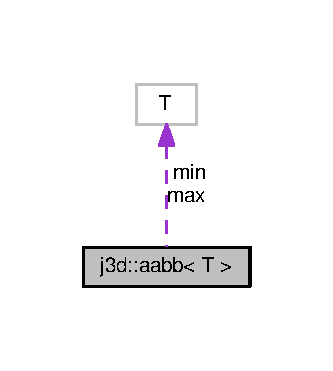
\includegraphics[width=160pt]{structj3d_1_1aabb__coll__graph}
\end{center}
\end{figure}
\subsection*{Public Member Functions}
\begin{DoxyCompactItemize}
\item 
\hypertarget{structj3d_1_1aabb_a7b6f5904f2c3a70e249aa863283e06f1}{}{\bfseries aabb} (const T \&\+\_\+min, const T \&\+\_\+max)\label{structj3d_1_1aabb_a7b6f5904f2c3a70e249aa863283e06f1}

\item 
\hypertarget{structj3d_1_1aabb_aa33a0a9b589417b802f02686b747a051}{}{\bfseries aabb} (const \hyperlink{structj3d_1_1aabb}{aabb}$<$ T $>$ \&a)\label{structj3d_1_1aabb_aa33a0a9b589417b802f02686b747a051}

\item 
\hypertarget{structj3d_1_1aabb_afd7c32cadccc09d11d99287a6d9962e3}{}\hyperlink{structj3d_1_1aabb}{aabb} \& {\bfseries operator=} (const \hyperlink{structj3d_1_1aabb}{aabb} \&a)\label{structj3d_1_1aabb_afd7c32cadccc09d11d99287a6d9962e3}

\item 
\hypertarget{structj3d_1_1aabb_a96053e9d9f442346c0a0af5f60501d7a}{}\hyperlink{structj3d_1_1aabb}{aabb} \& {\bfseries assign} (const T \&\+\_\+min, const T \&\+\_\+max)\label{structj3d_1_1aabb_a96053e9d9f442346c0a0af5f60501d7a}

\item 
\hypertarget{structj3d_1_1aabb_aaf4e2d4865cb1c822925d7c8a13dccb5}{}\hyperlink{structj3d_1_1aabb}{aabb} \& {\bfseries assign} (const \hyperlink{structj3d_1_1aabb}{aabb}$<$ T $>$ \&a)\label{structj3d_1_1aabb_aaf4e2d4865cb1c822925d7c8a13dccb5}

\end{DoxyCompactItemize}
\subsection*{Data Fields}
\begin{DoxyCompactItemize}
\item 
\hypertarget{structj3d_1_1aabb_a3e6d009ac4eea88d58c517d570e6f0fe}{}T {\bfseries min}\label{structj3d_1_1aabb_a3e6d009ac4eea88d58c517d570e6f0fe}

\item 
\hypertarget{structj3d_1_1aabb_adea255c8da2d6b7bc9e96cf86c1bff66}{}T {\bfseries max}\label{structj3d_1_1aabb_adea255c8da2d6b7bc9e96cf86c1bff66}

\end{DoxyCompactItemize}


The documentation for this struct was generated from the following file\+:\begin{DoxyCompactItemize}
\item 
/media/will/ratchet/\+Projects/\+J\+A\+W/j3d-\/demo/j3d/math/aabb.\+h\end{DoxyCompactItemize}

\hypertarget{classj3d_1_1core_1_1Batch}{}\section{j3d\+:\+:core\+:\+:Batch Class Reference}
\label{classj3d_1_1core_1_1Batch}\index{j3d\+::core\+::\+Batch@{j3d\+::core\+::\+Batch}}


Inheritance diagram for j3d\+:\+:core\+:\+:Batch\+:
\nopagebreak
\begin{figure}[H]
\begin{center}
\leavevmode
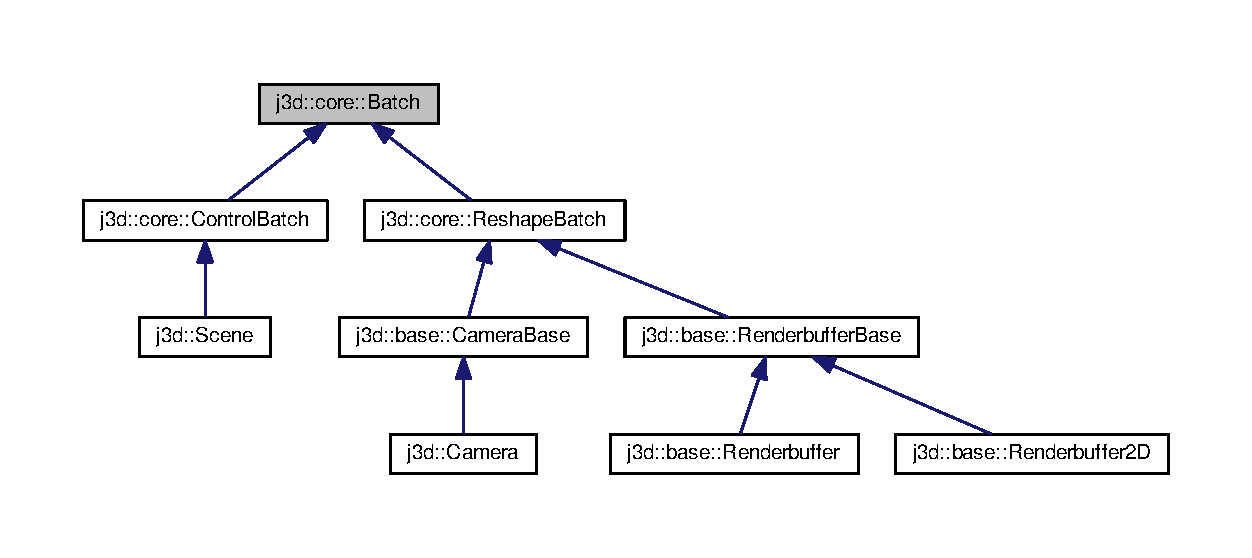
\includegraphics[width=350pt]{classj3d_1_1core_1_1Batch__inherit__graph}
\end{center}
\end{figure}
\subsection*{Public Member Functions}
\begin{DoxyCompactItemize}
\item 
\hypertarget{classj3d_1_1core_1_1Batch_a7f905c40386d89a6fa9392287ece7efc}{}{\bfseries Batch} (string id)\label{classj3d_1_1core_1_1Batch_a7f905c40386d89a6fa9392287ece7efc}

\end{DoxyCompactItemize}


The documentation for this class was generated from the following files\+:\begin{DoxyCompactItemize}
\item 
/media/will/ratchet/\+Projects/\+J\+A\+W/j3d-\/demo/j3d/core/batch.\+h\item 
/media/will/ratchet/\+Projects/\+J\+A\+W/j3d-\/demo/j3d/core/batch.\+cpp\end{DoxyCompactItemize}

\hypertarget{classj3d_1_1util_1_1batches}{}\section{j3d\+:\+:util\+:\+:batches Class Reference}
\label{classj3d_1_1util_1_1batches}\index{j3d\+::util\+::batches@{j3d\+::util\+::batches}}
\subsection*{Static Public Member Functions}
\begin{DoxyCompactItemize}
\item 
\hypertarget{classj3d_1_1util_1_1batches_a01edc7b298c2b11b0e0ddbbdf317b2ac}{}static void {\bfseries clear} ()\label{classj3d_1_1util_1_1batches_a01edc7b298c2b11b0e0ddbbdf317b2ac}

\item 
\hypertarget{classj3d_1_1util_1_1batches_aba61e72ad08835c16579b3ad76f18354}{}static void {\bfseries add} (string id, \hyperlink{classj3d_1_1core_1_1Batch}{batchobj} $\ast$)\label{classj3d_1_1util_1_1batches_aba61e72ad08835c16579b3ad76f18354}

\item 
\hypertarget{classj3d_1_1util_1_1batches_a1a9fc5b090b7b7370116042dd934dba5}{}static void {\bfseries remove} (string id, \hyperlink{classj3d_1_1core_1_1Batch}{batchobj} $\ast$)\label{classj3d_1_1util_1_1batches_a1a9fc5b090b7b7370116042dd934dba5}

\item 
\hypertarget{classj3d_1_1util_1_1batches_a57d33b974391d3376ae82616d9f48c5c}{}static batchgroup $\ast$ {\bfseries get} (string id)\label{classj3d_1_1util_1_1batches_a57d33b974391d3376ae82616d9f48c5c}

\end{DoxyCompactItemize}


The documentation for this class was generated from the following files\+:\begin{DoxyCompactItemize}
\item 
/media/will/ratchet/\+Projects/\+J\+A\+W/j3d-\/demo/j3d/util/batches.\+h\item 
/media/will/ratchet/\+Projects/\+J\+A\+W/j3d-\/demo/j3d/util/batches.\+cpp\end{DoxyCompactItemize}

\hypertarget{classj3d_1_1BoxMesh}{}\section{j3d\+:\+:Box\+Mesh Class Reference}
\label{classj3d_1_1BoxMesh}\index{j3d\+::\+Box\+Mesh@{j3d\+::\+Box\+Mesh}}


Inheritance diagram for j3d\+:\+:Box\+Mesh\+:
\nopagebreak
\begin{figure}[H]
\begin{center}
\leavevmode
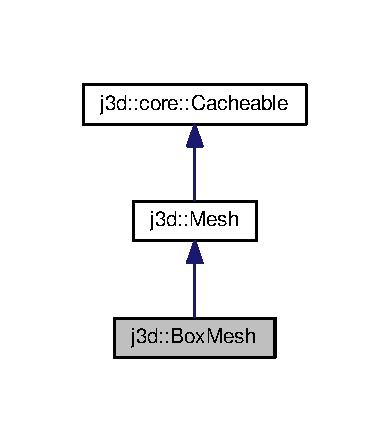
\includegraphics[width=187pt]{classj3d_1_1BoxMesh__inherit__graph}
\end{center}
\end{figure}


Collaboration diagram for j3d\+:\+:Box\+Mesh\+:
\nopagebreak
\begin{figure}[H]
\begin{center}
\leavevmode
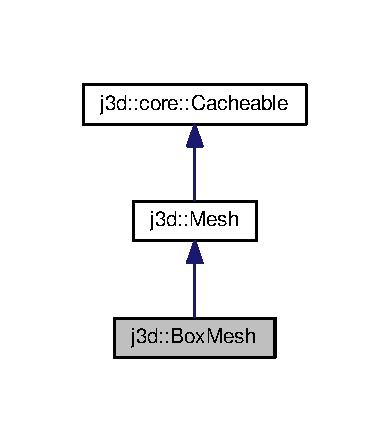
\includegraphics[width=187pt]{classj3d_1_1BoxMesh__coll__graph}
\end{center}
\end{figure}
\subsection*{Public Member Functions}
\begin{DoxyCompactItemize}
\item 
\hypertarget{classj3d_1_1BoxMesh_aa861551665f85cf83c18641d4b9e8bbf}{}{\bfseries Box\+Mesh} (const char $\ast$id, float s=1.\+0f)\label{classj3d_1_1BoxMesh_aa861551665f85cf83c18641d4b9e8bbf}

\item 
\hypertarget{classj3d_1_1BoxMesh_a85c6d0c1e9c3591a931c0d2c1d0c7af7}{}{\bfseries Box\+Mesh} (const char $\ast$id, float w, float l, float h)\label{classj3d_1_1BoxMesh_a85c6d0c1e9c3591a931c0d2c1d0c7af7}

\item 
\hypertarget{classj3d_1_1BoxMesh_a618cb439ab083e1ad5904181c50524ff}{}float {\bfseries size} () const \label{classj3d_1_1BoxMesh_a618cb439ab083e1ad5904181c50524ff}

\item 
\hypertarget{classj3d_1_1BoxMesh_ade973a1b8aa666e0eec946e79d053222}{}float {\bfseries width} () const \label{classj3d_1_1BoxMesh_ade973a1b8aa666e0eec946e79d053222}

\item 
\hypertarget{classj3d_1_1BoxMesh_a2f8d53a1d40fec083ddc74aa53b669c0}{}float {\bfseries length} () const \label{classj3d_1_1BoxMesh_a2f8d53a1d40fec083ddc74aa53b669c0}

\item 
\hypertarget{classj3d_1_1BoxMesh_a38e97c51f1e01240f170a73835305fd3}{}float {\bfseries height} () const \label{classj3d_1_1BoxMesh_a38e97c51f1e01240f170a73835305fd3}

\end{DoxyCompactItemize}
\subsection*{Additional Inherited Members}


The documentation for this class was generated from the following files\+:\begin{DoxyCompactItemize}
\item 
/media/will/ratchet/\+Projects/\+J\+A\+W/j3d-\/demo/j3d/mesh\+\_\+shapes.\+h\item 
/media/will/ratchet/\+Projects/\+J\+A\+W/j3d-\/demo/j3d/mesh\+\_\+shapes.\+cpp\end{DoxyCompactItemize}

\hypertarget{classj3d_1_1util_1_1cache}{}\section{j3d\+:\+:util\+:\+:cache Class Reference}
\label{classj3d_1_1util_1_1cache}\index{j3d\+::util\+::cache@{j3d\+::util\+::cache}}
\subsection*{Static Public Member Functions}
\begin{DoxyCompactItemize}
\item 
\hypertarget{classj3d_1_1util_1_1cache_a96f343ab4828f8b9537cec69bd84fd4c}{}static void {\bfseries clear} (bool call\+\_\+delete=true)\label{classj3d_1_1util_1_1cache_a96f343ab4828f8b9537cec69bd84fd4c}

\item 
\hypertarget{classj3d_1_1util_1_1cache_a43981d5d139f32dfd36df2366750a2f6}{}static void {\bfseries print} ()\label{classj3d_1_1util_1_1cache_a43981d5d139f32dfd36df2366750a2f6}

\item 
\hypertarget{classj3d_1_1util_1_1cache_a4bcd27cfa97120b04ce21c0f6f083a6f}{}static void {\bfseries print} (string id1)\label{classj3d_1_1util_1_1cache_a4bcd27cfa97120b04ce21c0f6f083a6f}

\item 
\hypertarget{classj3d_1_1util_1_1cache_a3638eaa514148a2c54047c133e38f01e}{}static bool {\bfseries group\+\_\+create} (string id1)\label{classj3d_1_1util_1_1cache_a3638eaa514148a2c54047c133e38f01e}

\item 
\hypertarget{classj3d_1_1util_1_1cache_af47c71316da35ae99901d40d48e2e5e6}{}static bool {\bfseries group\+\_\+destroy} (string id1, bool call\+\_\+delete=true)\label{classj3d_1_1util_1_1cache_af47c71316da35ae99901d40d48e2e5e6}

\item 
\hypertarget{classj3d_1_1util_1_1cache_a7872ddb1634db41aa71d107251bffa43}{}static const cachegroup $\ast$ {\bfseries group\+\_\+get} (string)\label{classj3d_1_1util_1_1cache_a7872ddb1634db41aa71d107251bffa43}

\item 
\hypertarget{classj3d_1_1util_1_1cache_a07e2249e65a51168fc3e61f2debe6d16}{}static bool {\bfseries group\+\_\+exists} (string id1, bool debug\+\_\+error=false)\label{classj3d_1_1util_1_1cache_a07e2249e65a51168fc3e61f2debe6d16}

\item 
\hypertarget{classj3d_1_1util_1_1cache_a0bcd23a06b0091138a6df26d50fabd33}{}static bool {\bfseries group\+\_\+empty} (string id1)\label{classj3d_1_1util_1_1cache_a0bcd23a06b0091138a6df26d50fabd33}

\item 
\hypertarget{classj3d_1_1util_1_1cache_ada855abd50d935400d308f7a35c90516}{}static size\+\_\+t {\bfseries group\+\_\+size} (string id1)\label{classj3d_1_1util_1_1cache_ada855abd50d935400d308f7a35c90516}

\item 
\hypertarget{classj3d_1_1util_1_1cache_a87f37b7e67ce434657c5b4ee49e7331f}{}static bool {\bfseries add} (string id1, string id2, \hyperlink{classj3d_1_1core_1_1Cacheable}{cacheitem} $\ast$, bool mkgrp=false)\label{classj3d_1_1util_1_1cache_a87f37b7e67ce434657c5b4ee49e7331f}

\item 
\hypertarget{classj3d_1_1util_1_1cache_a8721f6ba21a72fd86ad3041c46bb1322}{}static bool {\bfseries remove} (string id1, string id2, bool call\+\_\+delete=false)\label{classj3d_1_1util_1_1cache_a8721f6ba21a72fd86ad3041c46bb1322}

\item 
\hypertarget{classj3d_1_1util_1_1cache_a76cdbad15bd5161adab22ec8ca9607c7}{}static \hyperlink{classj3d_1_1core_1_1Cacheable}{cacheitem} $\ast$ {\bfseries get} (string id1, string id2)\label{classj3d_1_1util_1_1cache_a76cdbad15bd5161adab22ec8ca9607c7}

\item 
\hypertarget{classj3d_1_1util_1_1cache_ad7b73897796c88aabb7576f28071795c}{}static bool {\bfseries exists} (string id1, string id2, bool debug\+\_\+error=false)\label{classj3d_1_1util_1_1cache_ad7b73897796c88aabb7576f28071795c}

\item 
\hypertarget{classj3d_1_1util_1_1cache_a2cabdd0eaa408701ad188f64e58afb3e}{}static bool {\bfseries activate} (string id1, string id2)\label{classj3d_1_1util_1_1cache_a2cabdd0eaa408701ad188f64e58afb3e}

\item 
\hypertarget{classj3d_1_1util_1_1cache_a3939fb6419f93e062f29b6ec64eb6b63}{}static \hyperlink{classj3d_1_1core_1_1Cacheable}{cacheitem} $\ast$ {\bfseries active\+\_\+get} (string id1)\label{classj3d_1_1util_1_1cache_a3939fb6419f93e062f29b6ec64eb6b63}

\item 
\hypertarget{classj3d_1_1util_1_1cache_a61f5e6fabfa7f873b4ae44fc2f2d7692}{}static bool {\bfseries active\+\_\+exists} (string id1)\label{classj3d_1_1util_1_1cache_a61f5e6fabfa7f873b4ae44fc2f2d7692}

\end{DoxyCompactItemize}


The documentation for this class was generated from the following files\+:\begin{DoxyCompactItemize}
\item 
/media/will/ratchet/\+Projects/\+J\+A\+W/j3d-\/demo/j3d/util/cache.\+h\item 
/media/will/ratchet/\+Projects/\+J\+A\+W/j3d-\/demo/j3d/util/cache.\+cpp\end{DoxyCompactItemize}

\hypertarget{classj3d_1_1core_1_1Cacheable}{}\section{j3d\+:\+:core\+:\+:Cacheable Class Reference}
\label{classj3d_1_1core_1_1Cacheable}\index{j3d\+::core\+::\+Cacheable@{j3d\+::core\+::\+Cacheable}}


Inheritance diagram for j3d\+:\+:core\+:\+:Cacheable\+:
\nopagebreak
\begin{figure}[H]
\begin{center}
\leavevmode
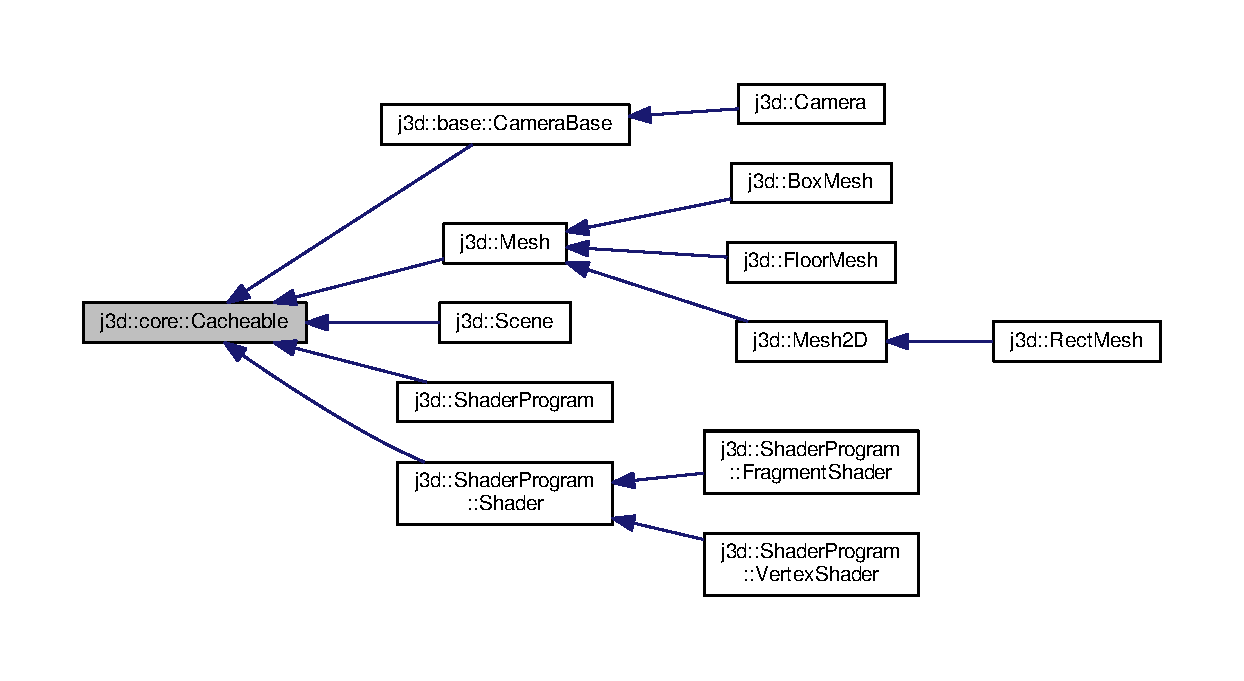
\includegraphics[width=350pt]{classj3d_1_1core_1_1Cacheable__inherit__graph}
\end{center}
\end{figure}
\subsection*{Public Member Functions}
\begin{DoxyCompactItemize}
\item 
\hypertarget{classj3d_1_1core_1_1Cacheable_ae1516b4f52227e68d6f58f19c4e365a1}{}{\bfseries Cacheable} (string id1, string id2, bool activate=true)\label{classj3d_1_1core_1_1Cacheable_ae1516b4f52227e68d6f58f19c4e365a1}

\item 
\hypertarget{classj3d_1_1core_1_1Cacheable_a027be45ddd07ac6d7fef24eb6b1d23e5}{}virtual void {\bfseries cache\+Activate} ()\label{classj3d_1_1core_1_1Cacheable_a027be45ddd07ac6d7fef24eb6b1d23e5}

\item 
\hypertarget{classj3d_1_1core_1_1Cacheable_a946246c166ba446dbded6dda27a669e3}{}const string \& {\bfseries cache\+Id} ()\label{classj3d_1_1core_1_1Cacheable_a946246c166ba446dbded6dda27a669e3}

\item 
\hypertarget{classj3d_1_1core_1_1Cacheable_aac11f2d4cc407ae3f8ea4c9f56712d9a}{}string {\bfseries cache\+Id\+Full} ()\label{classj3d_1_1core_1_1Cacheable_aac11f2d4cc407ae3f8ea4c9f56712d9a}

\end{DoxyCompactItemize}


The documentation for this class was generated from the following files\+:\begin{DoxyCompactItemize}
\item 
/media/will/ratchet/\+Projects/\+J\+A\+W/j3d-\/demo/j3d/core/cacheable.\+h\item 
/media/will/ratchet/\+Projects/\+J\+A\+W/j3d-\/demo/j3d/core/cacheable.\+cpp\end{DoxyCompactItemize}

\hypertarget{classj3d_1_1Camera}{}\section{j3d\+:\+:Camera Class Reference}
\label{classj3d_1_1Camera}\index{j3d\+::\+Camera@{j3d\+::\+Camera}}


Inheritance diagram for j3d\+:\+:Camera\+:
\nopagebreak
\begin{figure}[H]
\begin{center}
\leavevmode
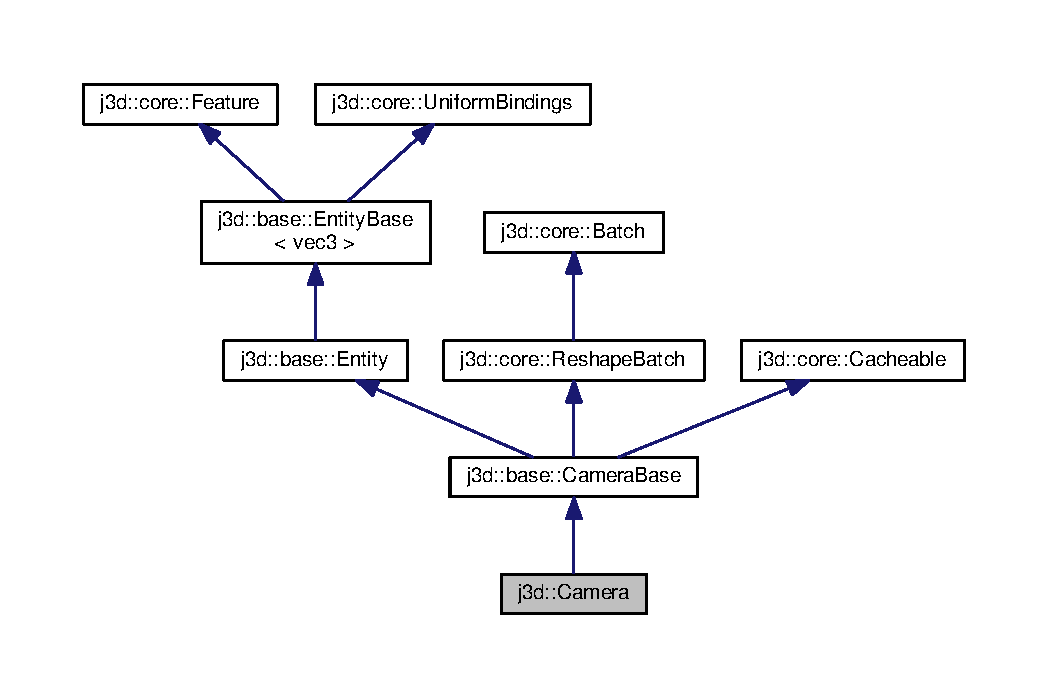
\includegraphics[width=350pt]{classj3d_1_1Camera__inherit__graph}
\end{center}
\end{figure}


Collaboration diagram for j3d\+:\+:Camera\+:
\nopagebreak
\begin{figure}[H]
\begin{center}
\leavevmode
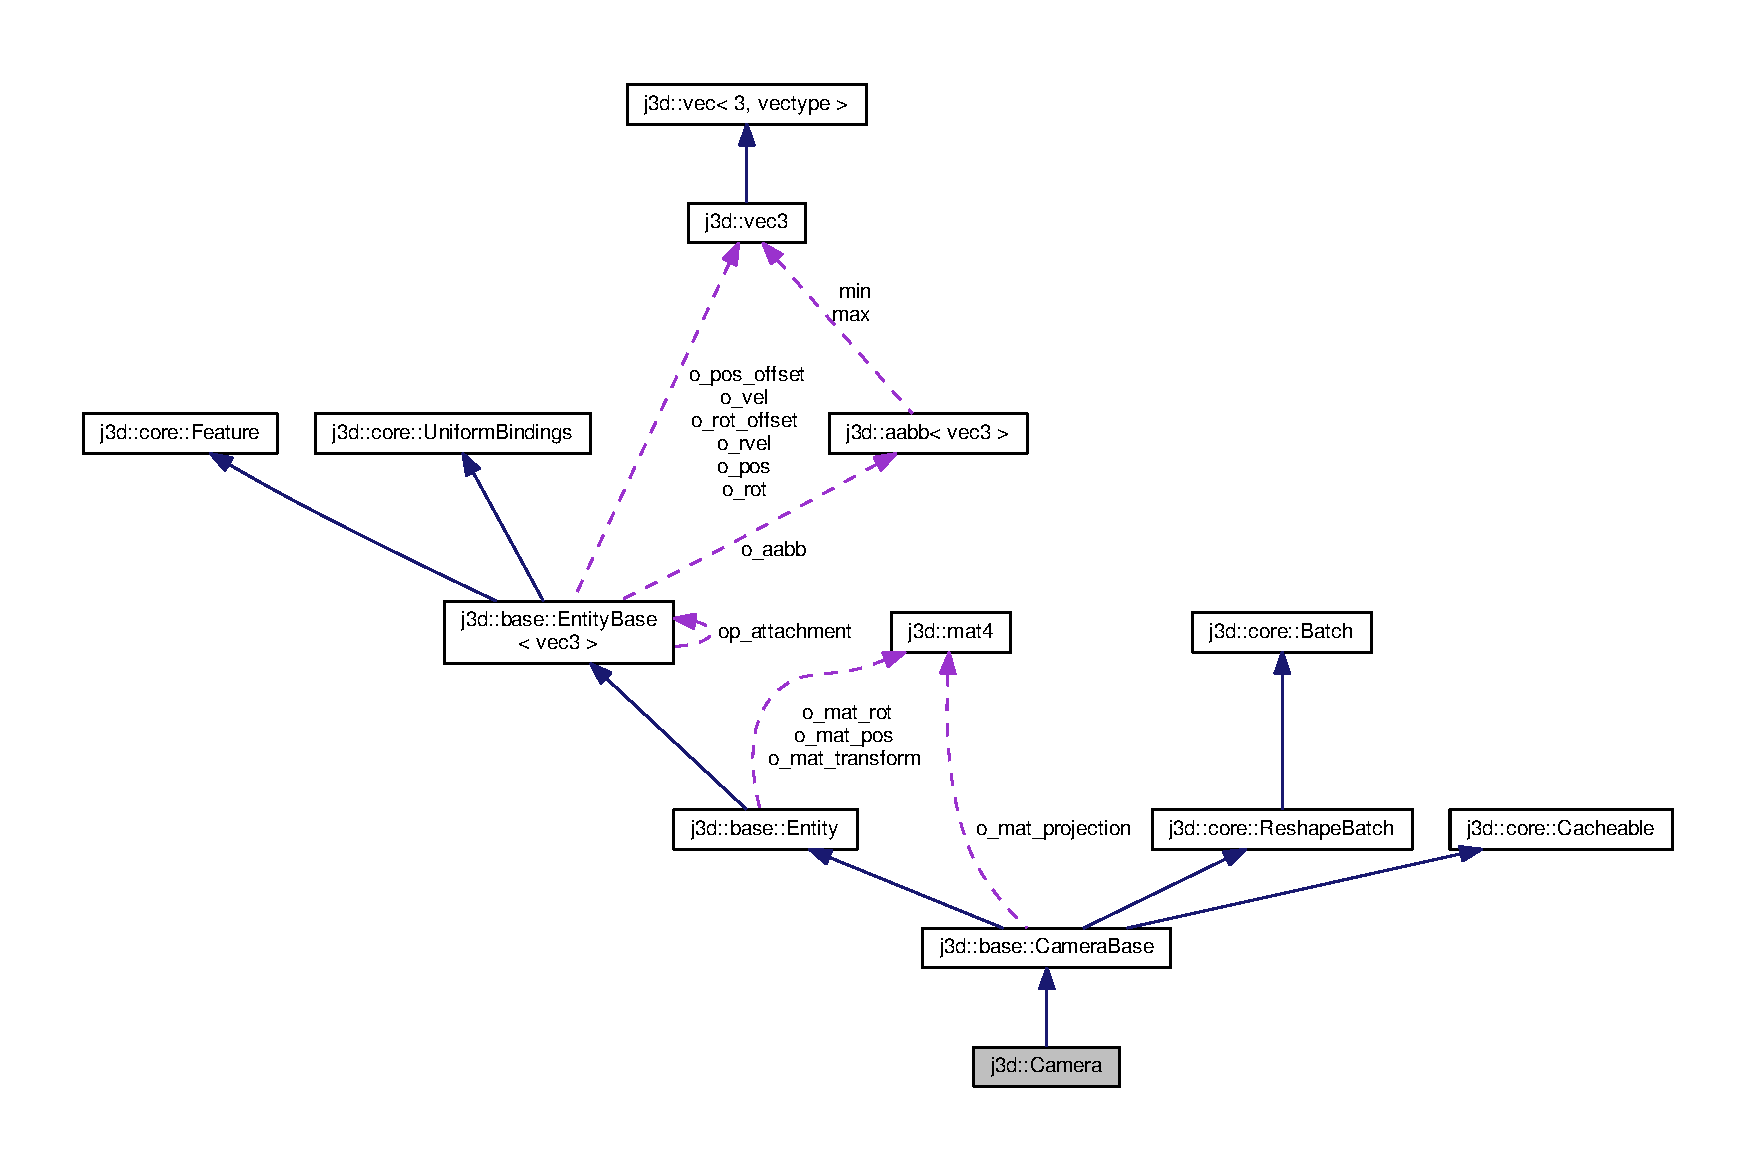
\includegraphics[width=350pt]{classj3d_1_1Camera__coll__graph}
\end{center}
\end{figure}
\subsection*{Public Member Functions}
\begin{DoxyCompactItemize}
\item 
\hypertarget{classj3d_1_1Camera_a5610d622d15122d22f23c3c03ad2aebf}{}{\bfseries Camera} (string id)\label{classj3d_1_1Camera_a5610d622d15122d22f23c3c03ad2aebf}

\item 
\hypertarget{classj3d_1_1Camera_a39e3f7635779c0213e8782e83a06fb9b}{}virtual \hyperlink{structj3d_1_1mat4}{mat4} \& {\bfseries projection} ()\label{classj3d_1_1Camera_a39e3f7635779c0213e8782e83a06fb9b}

\end{DoxyCompactItemize}
\subsection*{Additional Inherited Members}


The documentation for this class was generated from the following files\+:\begin{DoxyCompactItemize}
\item 
/media/will/ratchet/\+Projects/\+J\+A\+W/j3d-\/demo/j3d/camera.\+h\item 
/media/will/ratchet/\+Projects/\+J\+A\+W/j3d-\/demo/j3d/camera.\+cpp\end{DoxyCompactItemize}

\hypertarget{classj3d_1_1base_1_1CameraBase}{}\section{j3d\+:\+:base\+:\+:Camera\+Base Class Reference}
\label{classj3d_1_1base_1_1CameraBase}\index{j3d\+::base\+::\+Camera\+Base@{j3d\+::base\+::\+Camera\+Base}}


Inheritance diagram for j3d\+:\+:base\+:\+:Camera\+Base\+:
\nopagebreak
\begin{figure}[H]
\begin{center}
\leavevmode
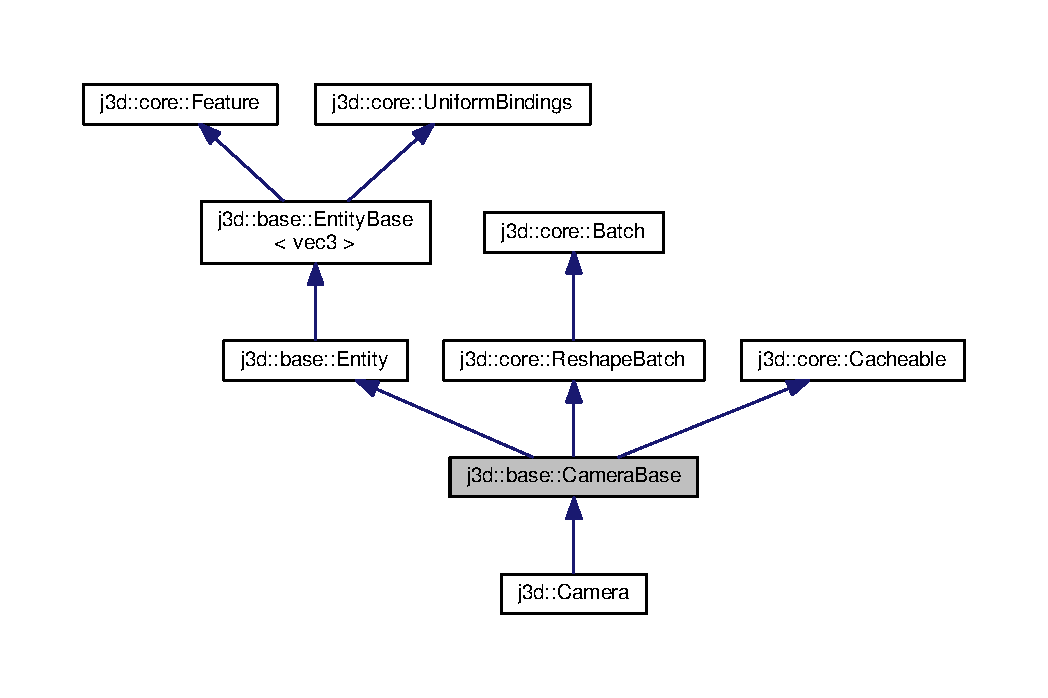
\includegraphics[width=350pt]{classj3d_1_1base_1_1CameraBase__inherit__graph}
\end{center}
\end{figure}


Collaboration diagram for j3d\+:\+:base\+:\+:Camera\+Base\+:
\nopagebreak
\begin{figure}[H]
\begin{center}
\leavevmode
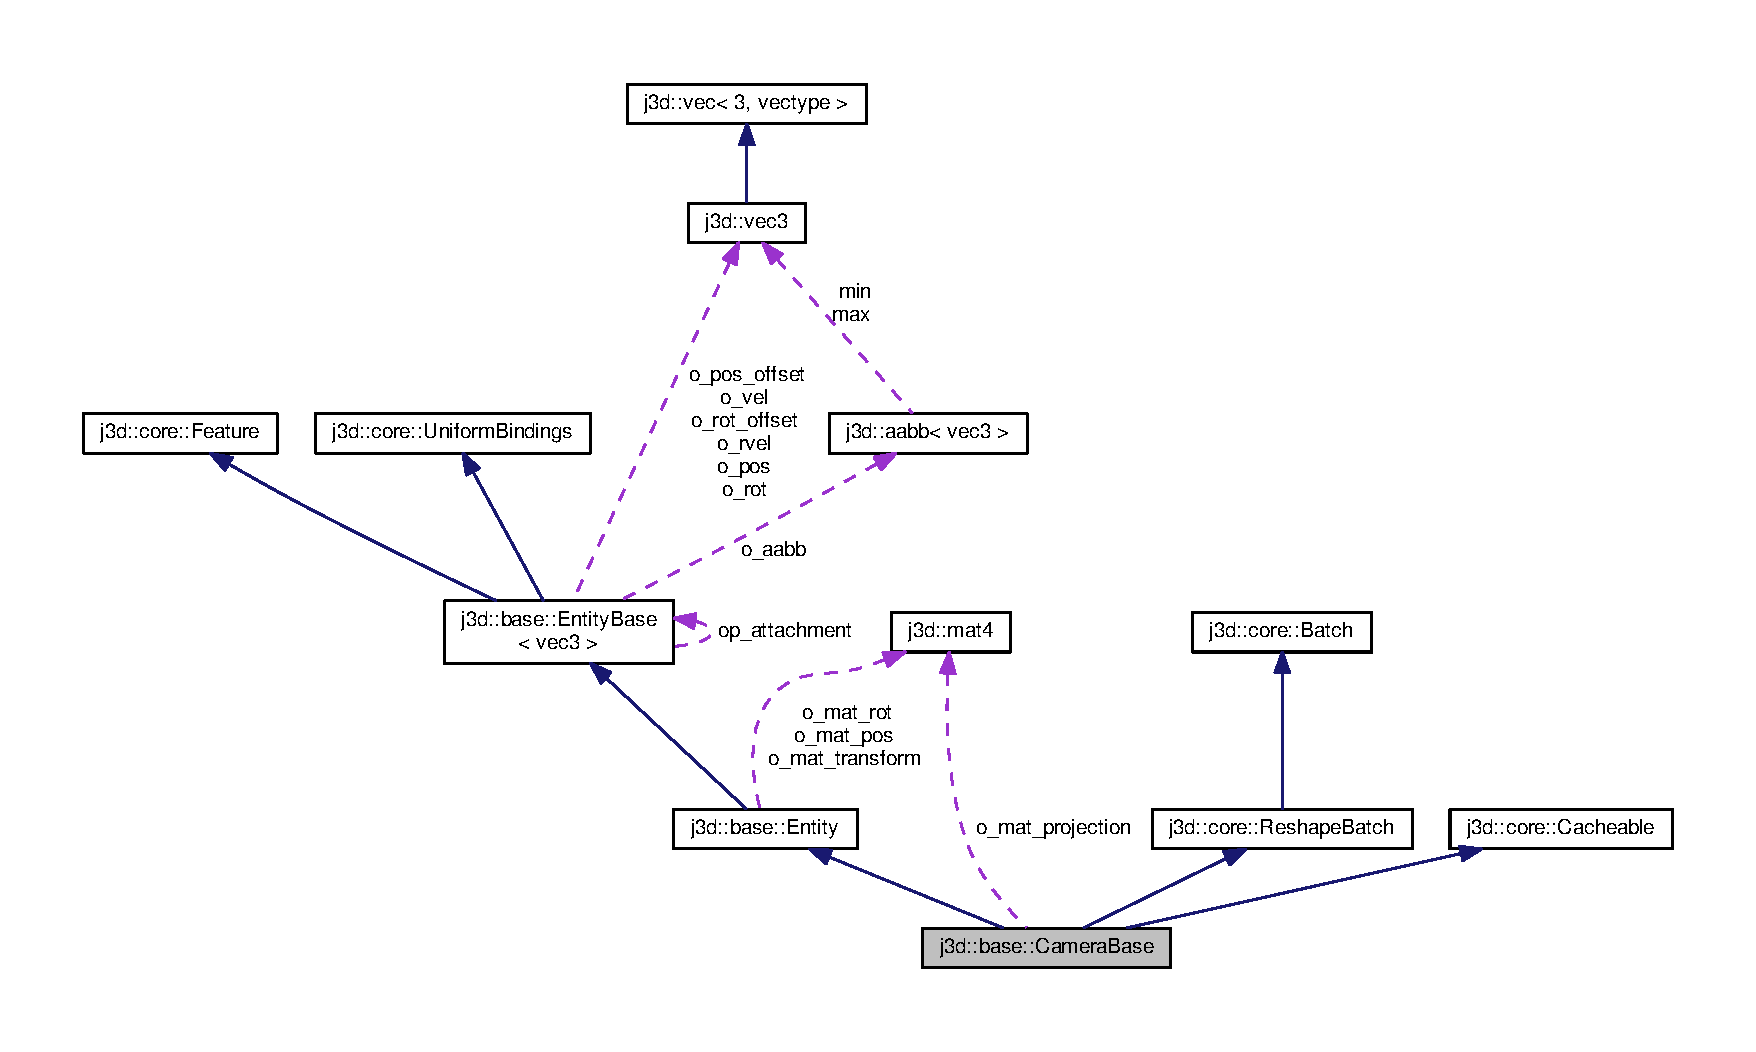
\includegraphics[width=350pt]{classj3d_1_1base_1_1CameraBase__coll__graph}
\end{center}
\end{figure}
\subsection*{Public Member Functions}
\begin{DoxyCompactItemize}
\item 
\hypertarget{classj3d_1_1base_1_1CameraBase_aa42dd40367d33cda277db47986ebe958}{}{\bfseries Camera\+Base} (string id, bool activate=true)\label{classj3d_1_1base_1_1CameraBase_aa42dd40367d33cda277db47986ebe958}

\item 
\hypertarget{classj3d_1_1base_1_1CameraBase_a707c9d371db5939b702c743e5bf41ae0}{}virtual void {\bfseries activate} ()\label{classj3d_1_1base_1_1CameraBase_a707c9d371db5939b702c743e5bf41ae0}

\item 
\hypertarget{classj3d_1_1base_1_1CameraBase_abc5d1d16fa0669c321e6735e6a774d58}{}virtual void {\bfseries reshape} (int w=0, int h=0)\label{classj3d_1_1base_1_1CameraBase_abc5d1d16fa0669c321e6735e6a774d58}

\item 
\hypertarget{classj3d_1_1base_1_1CameraBase_aaff78745b288d498b9b3f069f1170b35}{}virtual \hyperlink{structj3d_1_1mat4}{mat4} \& {\bfseries projection} ()=0\label{classj3d_1_1base_1_1CameraBase_aaff78745b288d498b9b3f069f1170b35}

\item 
\hypertarget{classj3d_1_1base_1_1CameraBase_a64e7991e4684abc92b502e9d9c780081}{}virtual \hyperlink{structj3d_1_1mat4}{mat4} \& {\bfseries transform} ()\label{classj3d_1_1base_1_1CameraBase_a64e7991e4684abc92b502e9d9c780081}

\item 
\hypertarget{classj3d_1_1base_1_1CameraBase_a03717e9181662ec952b99089382d6277}{}virtual void {\bfseries render} ()\label{classj3d_1_1base_1_1CameraBase_a03717e9181662ec952b99089382d6277}

\item 
\hypertarget{classj3d_1_1base_1_1CameraBase_aa5f08a22122e4f38191057337934bd98}{}\hyperlink{classj3d_1_1base_1_1CameraBase}{Camera\+Base} $\ast$ {\bfseries near} (float)\label{classj3d_1_1base_1_1CameraBase_aa5f08a22122e4f38191057337934bd98}

\item 
\hypertarget{classj3d_1_1base_1_1CameraBase_a11eb03e24c5ffc3a6f89ef120fb7a997}{}\hyperlink{classj3d_1_1base_1_1CameraBase}{Camera\+Base} $\ast$ {\bfseries far} (float)\label{classj3d_1_1base_1_1CameraBase_a11eb03e24c5ffc3a6f89ef120fb7a997}

\item 
\hypertarget{classj3d_1_1base_1_1CameraBase_a97019dfc8ed728db47311db65d9256cc}{}virtual float {\bfseries near} () const \label{classj3d_1_1base_1_1CameraBase_a97019dfc8ed728db47311db65d9256cc}

\item 
\hypertarget{classj3d_1_1base_1_1CameraBase_ad4dfe6fe4462e44ebc4cf105f683b626}{}virtual float {\bfseries far} () const \label{classj3d_1_1base_1_1CameraBase_ad4dfe6fe4462e44ebc4cf105f683b626}

\end{DoxyCompactItemize}
\subsection*{Static Public Attributes}
\begin{DoxyCompactItemize}
\item 
\hypertarget{classj3d_1_1base_1_1CameraBase_ac22a6ffdaa7b3b764b04df74a709e1c0}{}static const char constexpr $\ast$ {\bfseries J3\+D\+\_\+\+C\+A\+C\+H\+E\+\_\+\+I\+D} = \char`\"{}camera\char`\"{}\label{classj3d_1_1base_1_1CameraBase_ac22a6ffdaa7b3b764b04df74a709e1c0}

\end{DoxyCompactItemize}
\subsection*{Protected Attributes}
\begin{DoxyCompactItemize}
\item 
\hypertarget{classj3d_1_1base_1_1CameraBase_a23d168f7ff1a3574265f327b9f6db632}{}\hyperlink{structj3d_1_1mat4}{mat4} {\bfseries o\+\_\+mat\+\_\+projection}\label{classj3d_1_1base_1_1CameraBase_a23d168f7ff1a3574265f327b9f6db632}

\item 
\hypertarget{classj3d_1_1base_1_1CameraBase_a80964876077f13e779d762015b3f0b93}{}float {\bfseries o\+\_\+near}\label{classj3d_1_1base_1_1CameraBase_a80964876077f13e779d762015b3f0b93}

\item 
\hypertarget{classj3d_1_1base_1_1CameraBase_ae0a16fcd9438bca468226f3e6d1b3022}{}float {\bfseries o\+\_\+far}\label{classj3d_1_1base_1_1CameraBase_ae0a16fcd9438bca468226f3e6d1b3022}

\item 
\hypertarget{classj3d_1_1base_1_1CameraBase_a444f7e015d1e3ddba872796bc664957a}{}string {\bfseries o\+\_\+uniform\+\_\+id}\label{classj3d_1_1base_1_1CameraBase_a444f7e015d1e3ddba872796bc664957a}

\end{DoxyCompactItemize}


The documentation for this class was generated from the following files\+:\begin{DoxyCompactItemize}
\item 
/media/will/ratchet/\+Projects/\+J\+A\+W/j3d-\/demo/j3d/base/camera\+\_\+base.\+h\item 
/media/will/ratchet/\+Projects/\+J\+A\+W/j3d-\/demo/j3d/base/camera\+\_\+base.\+cpp\end{DoxyCompactItemize}

\hypertarget{structj3d_1_1collision}{}\section{j3d\+:\+:collision Struct Reference}
\label{structj3d_1_1collision}\index{j3d\+::collision@{j3d\+::collision}}
\subsection*{Static Public Member Functions}
\begin{DoxyCompactItemize}
\item 
\hypertarget{structj3d_1_1collision_a61a325d2a43ed604b4e95f9b063be6e0}{}static bool {\bfseries ray\+\_\+aabb} (\hyperlink{structj3d_1_1ray3}{ray3}, const \hyperlink{structj3d_1_1aabb}{aabb3} \&)\label{structj3d_1_1collision_a61a325d2a43ed604b4e95f9b063be6e0}

\end{DoxyCompactItemize}


The documentation for this struct was generated from the following files\+:\begin{DoxyCompactItemize}
\item 
/media/will/ratchet/\+Projects/\+J\+A\+W/j3d-\/demo/j3d/math/collision.\+h\item 
/media/will/ratchet/\+Projects/\+J\+A\+W/j3d-\/demo/j3d/math/collision.\+cpp\end{DoxyCompactItemize}

\hypertarget{structj3d_1_1Config}{}\section{j3d\+:\+:Config Struct Reference}
\label{structj3d_1_1Config}\index{j3d\+::\+Config@{j3d\+::\+Config}}
\subsection*{Public Member Functions}
\begin{DoxyCompactItemize}
\item 
\hypertarget{structj3d_1_1Config_ad6a6a5aea25774288fbc964e69c10479}{}void {\bfseries reset} ()\label{structj3d_1_1Config_ad6a6a5aea25774288fbc964e69c10479}

\end{DoxyCompactItemize}
\subsection*{Data Fields}
\begin{DoxyCompactItemize}
\item 
\hypertarget{structj3d_1_1Config_aa7b9ae8b5a98e9b893dcf3326c1760bc}{}int {\bfseries argc}\label{structj3d_1_1Config_aa7b9ae8b5a98e9b893dcf3326c1760bc}

\item 
\hypertarget{structj3d_1_1Config_a33ac9f8e35250cb132a7c7a047aee219}{}char $\ast$$\ast$ {\bfseries argv}\label{structj3d_1_1Config_a33ac9f8e35250cb132a7c7a047aee219}

\item 
\hypertarget{structj3d_1_1Config_ae2c29e54bce2307cf111f1138fda5ab4}{}int {\bfseries window\+\_\+width}\label{structj3d_1_1Config_ae2c29e54bce2307cf111f1138fda5ab4}

\item 
\hypertarget{structj3d_1_1Config_a937f9c8e0929068391850a74d0dea376}{}int {\bfseries window\+\_\+height}\label{structj3d_1_1Config_a937f9c8e0929068391850a74d0dea376}

\item 
\hypertarget{structj3d_1_1Config_a45574d8720a49b6f86fb1c9407167f54}{}int {\bfseries window\+\_\+start\+\_\+x}\label{structj3d_1_1Config_a45574d8720a49b6f86fb1c9407167f54}

\item 
\hypertarget{structj3d_1_1Config_a3248a51713dd5a62bcfc12b599c5a395}{}int {\bfseries window\+\_\+start\+\_\+y}\label{structj3d_1_1Config_a3248a51713dd5a62bcfc12b599c5a395}

\item 
\hypertarget{structj3d_1_1Config_a66bacc300d2b46f7c21fe4d6e6d4bb5d}{}string {\bfseries window\+\_\+title}\label{structj3d_1_1Config_a66bacc300d2b46f7c21fe4d6e6d4bb5d}

\item 
\hypertarget{structj3d_1_1Config_a43d09e324b507086dd8cdf0d04c03744}{}float {\bfseries mouse\+\_\+buffer\+\_\+time}\label{structj3d_1_1Config_a43d09e324b507086dd8cdf0d04c03744}

\item 
\hypertarget{structj3d_1_1Config_ab89ca062f159384bf903355fe5cf7b10}{}float {\bfseries render\+\_\+distance\+\_\+near}\label{structj3d_1_1Config_ab89ca062f159384bf903355fe5cf7b10}

\item 
\hypertarget{structj3d_1_1Config_ad28996f8247f451f4677525458a77111}{}float {\bfseries render\+\_\+distance\+\_\+far}\label{structj3d_1_1Config_ad28996f8247f451f4677525458a77111}

\item 
\hypertarget{structj3d_1_1Config_a1152bbbb4b24dcdcc51875eca5ef7cc0}{}bool {\bfseries register\+\_\+atexit}\label{structj3d_1_1Config_a1152bbbb4b24dcdcc51875eca5ef7cc0}

\item 
\hypertarget{structj3d_1_1Config_ac04484824009cc547dd9691b5e4021b4}{}bool {\bfseries register\+\_\+sigint}\label{structj3d_1_1Config_ac04484824009cc547dd9691b5e4021b4}

\end{DoxyCompactItemize}


The documentation for this struct was generated from the following file\+:\begin{DoxyCompactItemize}
\item 
/media/will/ratchet/\+Projects/\+J\+A\+W/j3d-\/demo/j3d/config.\+h\end{DoxyCompactItemize}

\hypertarget{classj3d_1_1util_1_1control}{}\section{j3d\+:\+:util\+:\+:control Class Reference}
\label{classj3d_1_1util_1_1control}\index{j3d\+::util\+::control@{j3d\+::util\+::control}}
\subsection*{Static Public Member Functions}
\begin{DoxyCompactItemize}
\item 
\hypertarget{classj3d_1_1util_1_1control_ae0d5a3ff2b8996008cf8fb2edc59b792}{}static void {\bfseries init} ()\label{classj3d_1_1util_1_1control_ae0d5a3ff2b8996008cf8fb2edc59b792}

\item 
\hypertarget{classj3d_1_1util_1_1control_a1132c4adfea16e810e41a879c3452d34}{}static void {\bfseries update} ()\label{classj3d_1_1util_1_1control_a1132c4adfea16e810e41a879c3452d34}

\item 
\hypertarget{classj3d_1_1util_1_1control_a735d2f9044a9d39e4473909b3c1fde2c}{}static void {\bfseries on\+\_\+key\+\_\+down} (unsigned char k, int x, int y)\label{classj3d_1_1util_1_1control_a735d2f9044a9d39e4473909b3c1fde2c}

\item 
\hypertarget{classj3d_1_1util_1_1control_a99e0a79b62a2a811ba088ecbd13fd3e8}{}static void {\bfseries on\+\_\+key\+\_\+up} (unsigned char k, int x, int y)\label{classj3d_1_1util_1_1control_a99e0a79b62a2a811ba088ecbd13fd3e8}

\item 
\hypertarget{classj3d_1_1util_1_1control_af4136da90458b87664563f18d9917aa6}{}static void {\bfseries on\+\_\+special\+\_\+down} (int k, int x, int y)\label{classj3d_1_1util_1_1control_af4136da90458b87664563f18d9917aa6}

\item 
\hypertarget{classj3d_1_1util_1_1control_ad933332c37105d938c8292f818229cfe}{}static void {\bfseries on\+\_\+special\+\_\+up} (int k, int x, int y)\label{classj3d_1_1util_1_1control_ad933332c37105d938c8292f818229cfe}

\item 
\hypertarget{classj3d_1_1util_1_1control_a18670fd8b0f6663c0c014cd7660326c0}{}static void {\bfseries on\+\_\+mouse\+\_\+click} (int b, int s, int x, int y)\label{classj3d_1_1util_1_1control_a18670fd8b0f6663c0c014cd7660326c0}

\item 
\hypertarget{classj3d_1_1util_1_1control_ad1a7189d7e34a7d7d67063c992cad869}{}static void {\bfseries on\+\_\+mouse\+\_\+move} (int x, int y)\label{classj3d_1_1util_1_1control_ad1a7189d7e34a7d7d67063c992cad869}

\item 
\hypertarget{classj3d_1_1util_1_1control_a70ba20b8a559d004df3529ec5ac43da0}{}static bool {\bfseries key\+\_\+down} (unsigned char)\label{classj3d_1_1util_1_1control_a70ba20b8a559d004df3529ec5ac43da0}

\item 
\hypertarget{classj3d_1_1util_1_1control_a0051a4cf79d4f6f2f5fe4b552e6e927c}{}static bool {\bfseries special\+\_\+down} (int)\label{classj3d_1_1util_1_1control_a0051a4cf79d4f6f2f5fe4b552e6e927c}

\item 
\hypertarget{classj3d_1_1util_1_1control_a60de829699621b24dda45975e4d5575b}{}static bool {\bfseries keys\+\_\+down} (initializer\+\_\+list$<$ unsigned char $>$)\label{classj3d_1_1util_1_1control_a60de829699621b24dda45975e4d5575b}

\item 
\hypertarget{classj3d_1_1util_1_1control_a4b8e14fc1291d40fba2442e451236edd}{}static bool {\bfseries specials\+\_\+down} (initializer\+\_\+list$<$ int $>$)\label{classj3d_1_1util_1_1control_a4b8e14fc1291d40fba2442e451236edd}

\item 
\hypertarget{classj3d_1_1util_1_1control_a8519387af6a71de4d5e04290eaad2a4f}{}static bool {\bfseries combo} (initializer\+\_\+list$<$ int $>$, initializer\+\_\+list$<$ unsigned char $>$)\label{classj3d_1_1util_1_1control_a8519387af6a71de4d5e04290eaad2a4f}

\end{DoxyCompactItemize}


The documentation for this class was generated from the following files\+:\begin{DoxyCompactItemize}
\item 
/media/will/ratchet/\+Projects/\+J\+A\+W/j3d-\/demo/j3d/util/control.\+h\item 
/media/will/ratchet/\+Projects/\+J\+A\+W/j3d-\/demo/j3d/util/control.\+cpp\end{DoxyCompactItemize}

\hypertarget{classj3d_1_1core_1_1ControlBatch}{}\section{j3d\+:\+:core\+:\+:Control\+Batch Class Reference}
\label{classj3d_1_1core_1_1ControlBatch}\index{j3d\+::core\+::\+Control\+Batch@{j3d\+::core\+::\+Control\+Batch}}


Inheritance diagram for j3d\+:\+:core\+:\+:Control\+Batch\+:
\nopagebreak
\begin{figure}[H]
\begin{center}
\leavevmode
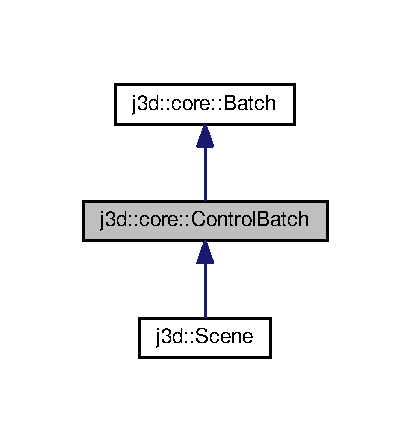
\includegraphics[width=197pt]{classj3d_1_1core_1_1ControlBatch__inherit__graph}
\end{center}
\end{figure}


Collaboration diagram for j3d\+:\+:core\+:\+:Control\+Batch\+:
\nopagebreak
\begin{figure}[H]
\begin{center}
\leavevmode
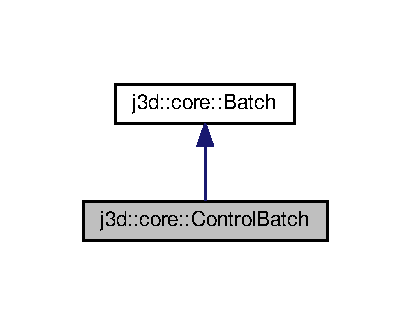
\includegraphics[width=197pt]{classj3d_1_1core_1_1ControlBatch__coll__graph}
\end{center}
\end{figure}
\subsection*{Public Member Functions}
\begin{DoxyCompactItemize}
\item 
\hypertarget{classj3d_1_1core_1_1ControlBatch_a91912cb466353b27388783f5ba36772a}{}virtual void {\bfseries on\+Key\+Down} (unsigned char key)\label{classj3d_1_1core_1_1ControlBatch_a91912cb466353b27388783f5ba36772a}

\item 
\hypertarget{classj3d_1_1core_1_1ControlBatch_a3da36986da46c72e4546bc6a41097862}{}virtual void {\bfseries on\+Key\+Down} (unsigned char key, int x, int y)\label{classj3d_1_1core_1_1ControlBatch_a3da36986da46c72e4546bc6a41097862}

\item 
\hypertarget{classj3d_1_1core_1_1ControlBatch_af28700dc578d720005442cd6f66d411a}{}virtual void {\bfseries on\+Key\+Up} (unsigned char key)\label{classj3d_1_1core_1_1ControlBatch_af28700dc578d720005442cd6f66d411a}

\item 
\hypertarget{classj3d_1_1core_1_1ControlBatch_ac8a055024f03e669bbb7ffdf2aafd747}{}virtual void {\bfseries on\+Key\+Up} (unsigned char key, int x, int y)\label{classj3d_1_1core_1_1ControlBatch_ac8a055024f03e669bbb7ffdf2aafd747}

\item 
\hypertarget{classj3d_1_1core_1_1ControlBatch_a68b3d00ca4ac0cbd3ff6306069002d79}{}virtual void {\bfseries on\+Special\+Down} (int key)\label{classj3d_1_1core_1_1ControlBatch_a68b3d00ca4ac0cbd3ff6306069002d79}

\item 
\hypertarget{classj3d_1_1core_1_1ControlBatch_a83487b7d6cdb4cdf1471be56dbc99afd}{}virtual void {\bfseries on\+Special\+Down} (int key, int x, int y)\label{classj3d_1_1core_1_1ControlBatch_a83487b7d6cdb4cdf1471be56dbc99afd}

\item 
\hypertarget{classj3d_1_1core_1_1ControlBatch_a6b4c76c0ea6bfe9a52993217349214ec}{}virtual void {\bfseries on\+Special\+Up} (int key)\label{classj3d_1_1core_1_1ControlBatch_a6b4c76c0ea6bfe9a52993217349214ec}

\item 
\hypertarget{classj3d_1_1core_1_1ControlBatch_a948cd5e98a6c9776acfdad2c1d3c9c6d}{}virtual void {\bfseries on\+Special\+Up} (int key, int x, int y)\label{classj3d_1_1core_1_1ControlBatch_a948cd5e98a6c9776acfdad2c1d3c9c6d}

\item 
\hypertarget{classj3d_1_1core_1_1ControlBatch_a8bd9107b6342c4a242df74b54b63fe94}{}virtual void {\bfseries on\+Mouse\+Down} (int button)\label{classj3d_1_1core_1_1ControlBatch_a8bd9107b6342c4a242df74b54b63fe94}

\item 
\hypertarget{classj3d_1_1core_1_1ControlBatch_a0e41ceda73ba5c3fb64c7b53bafbe0ca}{}virtual void {\bfseries on\+Mouse\+Down} (int button, int x, int y)\label{classj3d_1_1core_1_1ControlBatch_a0e41ceda73ba5c3fb64c7b53bafbe0ca}

\item 
\hypertarget{classj3d_1_1core_1_1ControlBatch_a2549bd9078646035cd5039318165c778}{}virtual void {\bfseries on\+Mouse\+Up} (int button)\label{classj3d_1_1core_1_1ControlBatch_a2549bd9078646035cd5039318165c778}

\item 
\hypertarget{classj3d_1_1core_1_1ControlBatch_aa29fdf4e8ab857895888f09df55546df}{}virtual void {\bfseries on\+Mouse\+Up} (int button, int x, int y)\label{classj3d_1_1core_1_1ControlBatch_aa29fdf4e8ab857895888f09df55546df}

\item 
\hypertarget{classj3d_1_1core_1_1ControlBatch_a16c72c07ca11e4278ae19165db3ee491}{}virtual void {\bfseries on\+Mouse\+Move} (int x, int y, int old\+\_\+x, int old\+\_\+y)\label{classj3d_1_1core_1_1ControlBatch_a16c72c07ca11e4278ae19165db3ee491}

\end{DoxyCompactItemize}
\subsection*{Static Public Attributes}
\begin{DoxyCompactItemize}
\item 
\hypertarget{classj3d_1_1core_1_1ControlBatch_a192511d7e9b7aca1d655c1bbb78d02bf}{}static const char constexpr $\ast$ {\bfseries J3\+D\+\_\+\+B\+A\+T\+C\+H\+\_\+\+I\+D} = \char`\"{}j3d\+\_\+control\char`\"{}\label{classj3d_1_1core_1_1ControlBatch_a192511d7e9b7aca1d655c1bbb78d02bf}

\end{DoxyCompactItemize}


The documentation for this class was generated from the following file\+:\begin{DoxyCompactItemize}
\item 
/media/will/ratchet/\+Projects/\+J\+A\+W/j3d-\/demo/j3d/core/control\+\_\+batch.\+h\end{DoxyCompactItemize}

\hypertarget{classCube}{}\section{Cube Class Reference}
\label{classCube}\index{Cube@{Cube}}


Inheritance diagram for Cube\+:
\nopagebreak
\begin{figure}[H]
\begin{center}
\leavevmode
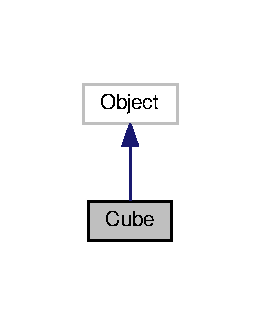
\includegraphics[width=125pt]{classCube__inherit__graph}
\end{center}
\end{figure}


Collaboration diagram for Cube\+:
\nopagebreak
\begin{figure}[H]
\begin{center}
\leavevmode
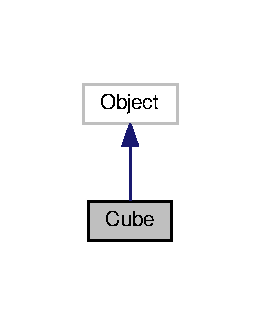
\includegraphics[width=125pt]{classCube__coll__graph}
\end{center}
\end{figure}


The documentation for this class was generated from the following file\+:\begin{DoxyCompactItemize}
\item 
/media/will/ratchet/\+Projects/\+J\+A\+W/j3d-\/demo/demo/cube.\+h\end{DoxyCompactItemize}

\hypertarget{classj3d_1_1util_1_1cycle}{}\section{j3d\+:\+:util\+:\+:cycle Class Reference}
\label{classj3d_1_1util_1_1cycle}\index{j3d\+::util\+::cycle@{j3d\+::util\+::cycle}}
\subsection*{Static Public Member Functions}
\begin{DoxyCompactItemize}
\item 
\hypertarget{classj3d_1_1util_1_1cycle_a3c9eb089570f6897eb7e303679a6a867}{}static float {\bfseries delta} ()\label{classj3d_1_1util_1_1cycle_a3c9eb089570f6897eb7e303679a6a867}

\item 
\hypertarget{classj3d_1_1util_1_1cycle_a9ed1e1d22182bac0404f52ab2083c0f3}{}static double {\bfseries deltad} ()\label{classj3d_1_1util_1_1cycle_a9ed1e1d22182bac0404f52ab2083c0f3}

\item 
\hypertarget{classj3d_1_1util_1_1cycle_a85dc3fdc4ede3888741a1960922959c4}{}{\footnotesize template$<$class T $>$ }\\static T {\bfseries delta} ()\label{classj3d_1_1util_1_1cycle_a85dc3fdc4ede3888741a1960922959c4}

\item 
\hypertarget{classj3d_1_1util_1_1cycle_a2de071a89920dd94d1a95a07011f9c83}{}static bool {\bfseries advise\+\_\+reshape} ()\label{classj3d_1_1util_1_1cycle_a2de071a89920dd94d1a95a07011f9c83}

\item 
\hypertarget{classj3d_1_1util_1_1cycle_ac13cb8285c8733e94549b8d271bc2cef}{}static bool {\bfseries advise\+\_\+quit} ()\label{classj3d_1_1util_1_1cycle_ac13cb8285c8733e94549b8d271bc2cef}

\item 
\hypertarget{classj3d_1_1util_1_1cycle_a6262059e5700e2b53cd368837a9db1a7}{}static void {\bfseries advise\+\_\+reshape} (bool)\label{classj3d_1_1util_1_1cycle_a6262059e5700e2b53cd368837a9db1a7}

\item 
\hypertarget{classj3d_1_1util_1_1cycle_aedf7800808af7d2feaff0c739fd42e06}{}static void {\bfseries advise\+\_\+quit} (bool)\label{classj3d_1_1util_1_1cycle_aedf7800808af7d2feaff0c739fd42e06}

\end{DoxyCompactItemize}
\subsection*{Friends}
\begin{DoxyCompactItemize}
\item 
\hypertarget{classj3d_1_1util_1_1cycle_a574ac12c3886b26b9da6eacbf4ad9a80}{}class {\bfseries j3d\+::engine}\label{classj3d_1_1util_1_1cycle_a574ac12c3886b26b9da6eacbf4ad9a80}

\end{DoxyCompactItemize}


The documentation for this class was generated from the following files\+:\begin{DoxyCompactItemize}
\item 
/media/will/ratchet/\+Projects/\+J\+A\+W/j3d-\/demo/j3d/util/cycle.\+h\item 
/media/will/ratchet/\+Projects/\+J\+A\+W/j3d-\/demo/j3d/util/cycle.\+cpp\end{DoxyCompactItemize}

\hypertarget{classj3d_1_1util_1_1debug}{}\section{j3d\+:\+:util\+:\+:debug Class Reference}
\label{classj3d_1_1util_1_1debug}\index{j3d\+::util\+::debug@{j3d\+::util\+::debug}}
\subsection*{Static Public Member Functions}
\begin{DoxyCompactItemize}
\item 
\hypertarget{classj3d_1_1util_1_1debug_a46c2655b361d999a38ea6a5fda13a44c}{}static void {\bfseries write} (string file, string func, int line, string color, string title, string message, bool status=false)\label{classj3d_1_1util_1_1debug_a46c2655b361d999a38ea6a5fda13a44c}

\item 
\hypertarget{classj3d_1_1util_1_1debug_a5600d9143916c312ac09bc0d67c61d02}{}static void {\bfseries status} (string color, string status)\label{classj3d_1_1util_1_1debug_a5600d9143916c312ac09bc0d67c61d02}

\item 
\hypertarget{classj3d_1_1util_1_1debug_afa07b0598be16dc230a2e593964b8b85}{}static void {\bfseries status} (string color, string status, string color2, string message)\label{classj3d_1_1util_1_1debug_afa07b0598be16dc230a2e593964b8b85}

\item 
\hypertarget{classj3d_1_1util_1_1debug_a8566fe1326765aacc893c20420f5f267}{}static void {\bfseries push\+\_\+tier} ()\label{classj3d_1_1util_1_1debug_a8566fe1326765aacc893c20420f5f267}

\item 
\hypertarget{classj3d_1_1util_1_1debug_ae0b373c08e861840e7f072ffa71ef8fa}{}static void {\bfseries pop\+\_\+tier} ()\label{classj3d_1_1util_1_1debug_ae0b373c08e861840e7f072ffa71ef8fa}

\item 
\hypertarget{classj3d_1_1util_1_1debug_a77da257ea99b156f3d7561dd6255a3e4}{}static void {\bfseries level} (int)\label{classj3d_1_1util_1_1debug_a77da257ea99b156f3d7561dd6255a3e4}

\item 
\hypertarget{classj3d_1_1util_1_1debug_a66323699c0723165c71b31c332d05c15}{}static void {\bfseries colorize} (bool)\label{classj3d_1_1util_1_1debug_a66323699c0723165c71b31c332d05c15}

\item 
\hypertarget{classj3d_1_1util_1_1debug_a1b7e9c8c285e6966be743029a285ed9d}{}static void {\bfseries tier} (int)\label{classj3d_1_1util_1_1debug_a1b7e9c8c285e6966be743029a285ed9d}

\item 
\hypertarget{classj3d_1_1util_1_1debug_a4c0562648a49a4d282cfb0db5876a68e}{}static int {\bfseries level} ()\label{classj3d_1_1util_1_1debug_a4c0562648a49a4d282cfb0db5876a68e}

\item 
\hypertarget{classj3d_1_1util_1_1debug_afe537602d6588fffd6e3785d072e2db3}{}static bool {\bfseries colorize} ()\label{classj3d_1_1util_1_1debug_afe537602d6588fffd6e3785d072e2db3}

\item 
\hypertarget{classj3d_1_1util_1_1debug_a489d891cdb7ed59e017e7db6029d9687}{}static int {\bfseries tier} ()\label{classj3d_1_1util_1_1debug_a489d891cdb7ed59e017e7db6029d9687}

\end{DoxyCompactItemize}


The documentation for this class was generated from the following files\+:\begin{DoxyCompactItemize}
\item 
/media/will/ratchet/\+Projects/\+J\+A\+W/j3d-\/demo/j3d/util/debug.\+h\item 
/media/will/ratchet/\+Projects/\+J\+A\+W/j3d-\/demo/j3d/util/debug.\+cpp\end{DoxyCompactItemize}

\hypertarget{structj3d_1_1util_1_1debug__settings}{}\section{j3d\+:\+:util\+:\+:debug\+\_\+settings Struct Reference}
\label{structj3d_1_1util_1_1debug__settings}\index{j3d\+::util\+::debug\+\_\+settings@{j3d\+::util\+::debug\+\_\+settings}}
\subsection*{Static Public Attributes}
\begin{DoxyCompactItemize}
\item 
\hypertarget{structj3d_1_1util_1_1debug__settings_a842fb78bcd25827651da2bd61e7f784b}{}static int {\bfseries level}\label{structj3d_1_1util_1_1debug__settings_a842fb78bcd25827651da2bd61e7f784b}

\item 
\hypertarget{structj3d_1_1util_1_1debug__settings_a136dd77c4a0cc13e503409ad8b122b12}{}static bool {\bfseries colorize}\label{structj3d_1_1util_1_1debug__settings_a136dd77c4a0cc13e503409ad8b122b12}

\end{DoxyCompactItemize}


The documentation for this struct was generated from the following file\+:\begin{DoxyCompactItemize}
\item 
/media/will/ratchet/\+Projects/\+J\+A\+W/j3d-\/demo/j3d/util/debug.\+h\end{DoxyCompactItemize}

\hypertarget{classDemo}{}\section{Demo Class Reference}
\label{classDemo}\index{Demo@{Demo}}


Inheritance diagram for Demo\+:
\nopagebreak
\begin{figure}[H]
\begin{center}
\leavevmode
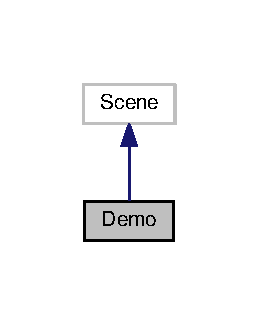
\includegraphics[width=124pt]{classDemo__inherit__graph}
\end{center}
\end{figure}


Collaboration diagram for Demo\+:
\nopagebreak
\begin{figure}[H]
\begin{center}
\leavevmode
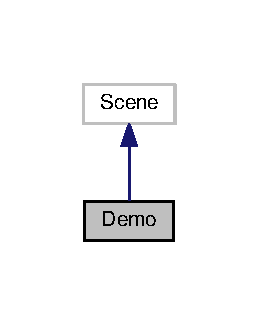
\includegraphics[width=124pt]{classDemo__coll__graph}
\end{center}
\end{figure}
\subsection*{Protected Member Functions}
\begin{DoxyCompactItemize}
\item 
\hypertarget{classDemo_acc38841a2fbde4d25340a3e6eb32e25d}{}void {\bfseries load} ()\label{classDemo_acc38841a2fbde4d25340a3e6eb32e25d}

\item 
\hypertarget{classDemo_ae09fe28d4f7a2db64da1850b3c9a05a0}{}void {\bfseries unload} ()\label{classDemo_ae09fe28d4f7a2db64da1850b3c9a05a0}

\item 
\hypertarget{classDemo_a88a7ddbf3a2abcb93ace999b607fae61}{}void {\bfseries update} ()\label{classDemo_a88a7ddbf3a2abcb93ace999b607fae61}

\item 
\hypertarget{classDemo_aeab99b8d2963cf21020d41fd99db023e}{}void {\bfseries on\+Key\+Down} (unsigned char)\label{classDemo_aeab99b8d2963cf21020d41fd99db023e}

\item 
\hypertarget{classDemo_aea65cbc08318f2a3e59c72f35fa9917b}{}void {\bfseries on\+Key\+Up} (unsigned char)\label{classDemo_aea65cbc08318f2a3e59c72f35fa9917b}

\item 
\hypertarget{classDemo_af452710deabb9393252eb9924eddd354}{}void {\bfseries on\+Mouse\+Up} (int, int, int)\label{classDemo_af452710deabb9393252eb9924eddd354}

\end{DoxyCompactItemize}


The documentation for this class was generated from the following files\+:\begin{DoxyCompactItemize}
\item 
/media/will/ratchet/\+Projects/\+J\+A\+W/j3d-\/demo/demo/demo.\+h\item 
/media/will/ratchet/\+Projects/\+J\+A\+W/j3d-\/demo/demo/demo.\+cpp\end{DoxyCompactItemize}

\hypertarget{classj3d_1_1base_1_1Display}{}\section{j3d\+:\+:base\+:\+:Display Class Reference}
\label{classj3d_1_1base_1_1Display}\index{j3d\+::base\+::\+Display@{j3d\+::base\+::\+Display}}
\subsection*{Public Member Functions}
\begin{DoxyCompactItemize}
\item 
\hypertarget{classj3d_1_1base_1_1Display_a4e83840b1b123cef2e51407519690612}{}virtual void {\bfseries loop} ()\label{classj3d_1_1base_1_1Display_a4e83840b1b123cef2e51407519690612}

\item 
\hypertarget{classj3d_1_1base_1_1Display_ae7f891cbe85bb44215a472368b34ce90}{}virtual void {\bfseries leave\+Loop} ()\label{classj3d_1_1base_1_1Display_ae7f891cbe85bb44215a472368b34ce90}

\item 
\hypertarget{classj3d_1_1base_1_1Display_a049e9fe3de7c97be0ff2f6c2f9036eb9}{}virtual void {\bfseries reshape} (int w, int h)\label{classj3d_1_1base_1_1Display_a049e9fe3de7c97be0ff2f6c2f9036eb9}

\item 
\hypertarget{classj3d_1_1base_1_1Display_a732bf03f4a598c8d3785e0f27c616b19}{}virtual void {\bfseries display} ()\label{classj3d_1_1base_1_1Display_a732bf03f4a598c8d3785e0f27c616b19}

\end{DoxyCompactItemize}
\subsection*{Static Public Member Functions}
\begin{DoxyCompactItemize}
\item 
\hypertarget{classj3d_1_1base_1_1Display_a8259059d2ac08fe08c19dfc677d3229b}{}static void {\bfseries on\+\_\+reshape} (int w, int h)\label{classj3d_1_1base_1_1Display_a8259059d2ac08fe08c19dfc677d3229b}

\item 
\hypertarget{classj3d_1_1base_1_1Display_ae1e111a7d45e13b4ae0e03fff9baaad9}{}static void {\bfseries on\+\_\+display} ()\label{classj3d_1_1base_1_1Display_ae1e111a7d45e13b4ae0e03fff9baaad9}

\end{DoxyCompactItemize}


The documentation for this class was generated from the following files\+:\begin{DoxyCompactItemize}
\item 
/media/will/ratchet/\+Projects/\+J\+A\+W/j3d-\/demo/j3d/base/display.\+h\item 
/media/will/ratchet/\+Projects/\+J\+A\+W/j3d-\/demo/j3d/base/display.\+cpp\end{DoxyCompactItemize}

\hypertarget{classj3d_1_1engine}{}\section{j3d\+:\+:engine Class Reference}
\label{classj3d_1_1engine}\index{j3d\+::engine@{j3d\+::engine}}
\subsection*{Static Public Member Functions}
\begin{DoxyCompactItemize}
\item 
\hypertarget{classj3d_1_1engine_aa554515fcafe40456ade1ecfe75ce7a6}{}static void {\bfseries init} (const \hyperlink{structj3d_1_1Config}{Config} \&)\label{classj3d_1_1engine_aa554515fcafe40456ade1ecfe75ce7a6}

\item 
\hypertarget{classj3d_1_1engine_a1828719b041858237f4c9bdf239eb911}{}static void {\bfseries quit} (int exit\+\_\+code=0)\label{classj3d_1_1engine_a1828719b041858237f4c9bdf239eb911}

\item 
\hypertarget{classj3d_1_1engine_a6ecc5e83a4e77eb359d0f9ad5239dd0d}{}static void {\bfseries run} ()\label{classj3d_1_1engine_a6ecc5e83a4e77eb359d0f9ad5239dd0d}

\item 
\hypertarget{classj3d_1_1engine_ac43220a1d72ecc64816d622507e782a1}{}static void {\bfseries atexit\+\_\+callback} ()\label{classj3d_1_1engine_ac43220a1d72ecc64816d622507e782a1}

\item 
\hypertarget{classj3d_1_1engine_aef0f91b305894f598dff9b0fd083dba9}{}static void {\bfseries sigint\+\_\+handler} (int)\label{classj3d_1_1engine_aef0f91b305894f598dff9b0fd083dba9}

\item 
\hypertarget{classj3d_1_1engine_a5bd62153776fc7e3e9506abc77c94c6a}{}static void {\bfseries update} ()\label{classj3d_1_1engine_a5bd62153776fc7e3e9506abc77c94c6a}

\item 
\hypertarget{classj3d_1_1engine_af71acaa1ef5bf7ccecf1bd3b668fe810}{}static bool {\bfseries initialized} ()\label{classj3d_1_1engine_af71acaa1ef5bf7ccecf1bd3b668fe810}

\item 
\hypertarget{classj3d_1_1engine_af54420f4bbf86ad0cb485cde01eaaf78}{}static \hyperlink{structj3d_1_1Config}{Config} $\ast$ {\bfseries config} ()\label{classj3d_1_1engine_af54420f4bbf86ad0cb485cde01eaaf78}

\item 
\hypertarget{classj3d_1_1engine_a150b65cbbf2ebf49090f489f266bbe54}{}static \hyperlink{classj3d_1_1base_1_1Display}{base\+::\+Display} $\ast$ {\bfseries display} ()\label{classj3d_1_1engine_a150b65cbbf2ebf49090f489f266bbe54}

\end{DoxyCompactItemize}


The documentation for this class was generated from the following files\+:\begin{DoxyCompactItemize}
\item 
/media/will/ratchet/\+Projects/\+J\+A\+W/j3d-\/demo/j3d/engine.\+h\item 
/media/will/ratchet/\+Projects/\+J\+A\+W/j3d-\/demo/j3d/engine.\+cpp\end{DoxyCompactItemize}

\hypertarget{classj3d_1_1base_1_1Entity}{}\section{j3d\+:\+:base\+:\+:Entity Class Reference}
\label{classj3d_1_1base_1_1Entity}\index{j3d\+::base\+::\+Entity@{j3d\+::base\+::\+Entity}}


Inheritance diagram for j3d\+:\+:base\+:\+:Entity\+:
\nopagebreak
\begin{figure}[H]
\begin{center}
\leavevmode
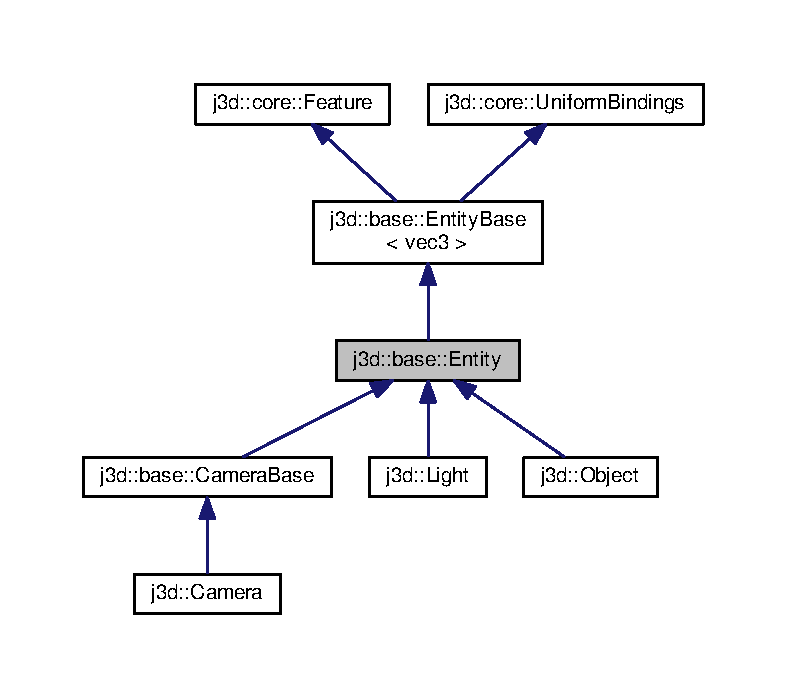
\includegraphics[width=350pt]{classj3d_1_1base_1_1Entity__inherit__graph}
\end{center}
\end{figure}


Collaboration diagram for j3d\+:\+:base\+:\+:Entity\+:
\nopagebreak
\begin{figure}[H]
\begin{center}
\leavevmode
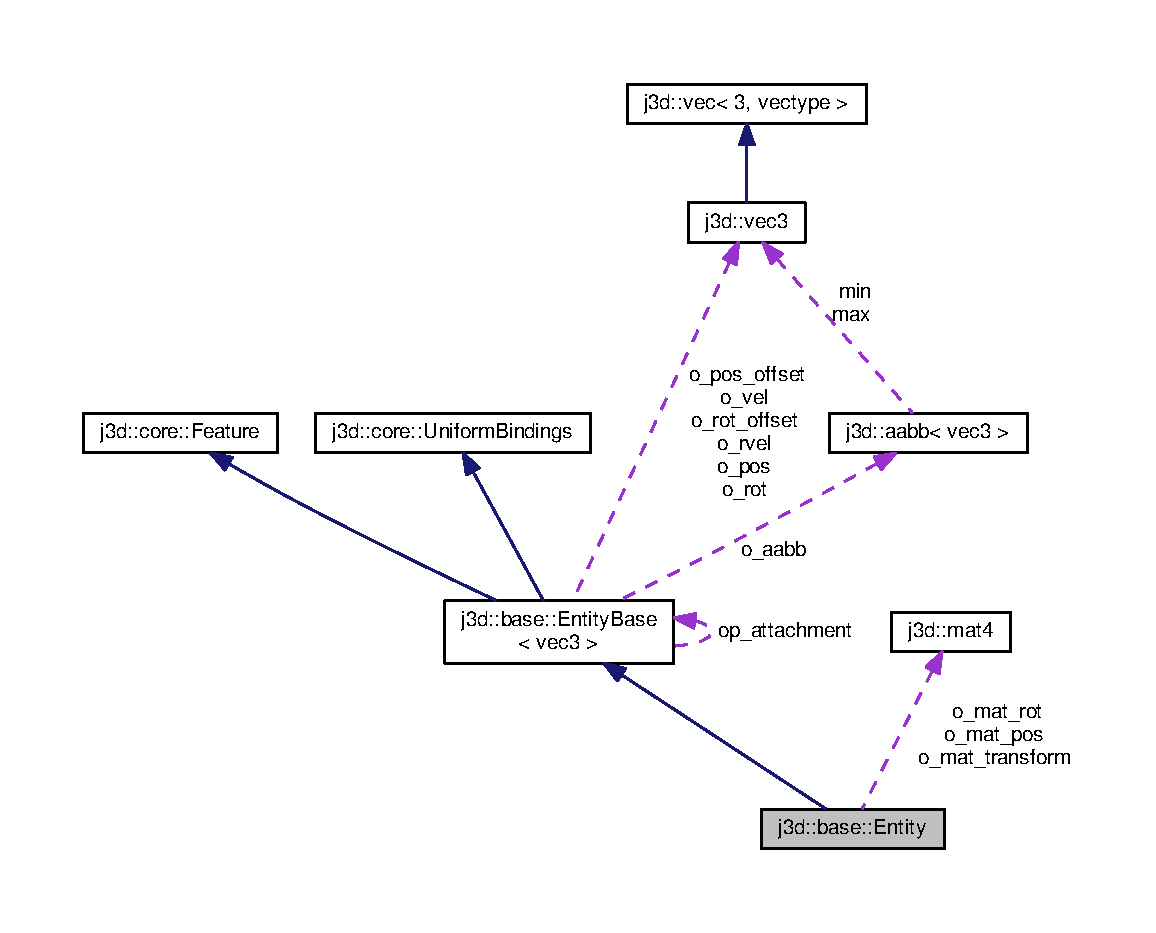
\includegraphics[width=350pt]{classj3d_1_1base_1_1Entity__coll__graph}
\end{center}
\end{figure}
\subsection*{Public Member Functions}
\begin{DoxyCompactItemize}
\item 
\hypertarget{classj3d_1_1base_1_1Entity_a1e26facf0f0b70e24c5255783bb70c8e}{}{\bfseries Entity} (string shader\+\_\+id)\label{classj3d_1_1base_1_1Entity_a1e26facf0f0b70e24c5255783bb70c8e}

\item 
\hypertarget{classj3d_1_1base_1_1Entity_af488650fced36d7d51450d5977e4d568}{}virtual void {\bfseries update} ()\label{classj3d_1_1base_1_1Entity_af488650fced36d7d51450d5977e4d568}

\item 
\hypertarget{classj3d_1_1base_1_1Entity_aa25b76f4e301dec12d4dabdac4c61d29}{}virtual \hyperlink{structj3d_1_1mat4}{mat4} \& {\bfseries transform} ()\label{classj3d_1_1base_1_1Entity_aa25b76f4e301dec12d4dabdac4c61d29}

\item 
\hypertarget{classj3d_1_1base_1_1Entity_aae96ef3ce4a8877cff2e6176cc2cbaa4}{}virtual \hyperlink{classj3d_1_1base_1_1Entity}{Entity} $\ast$ {\bfseries look\+At} (const \hyperlink{structj3d_1_1vec3}{vec3} \&)\label{classj3d_1_1base_1_1Entity_aae96ef3ce4a8877cff2e6176cc2cbaa4}

\item 
\hypertarget{classj3d_1_1base_1_1Entity_a5ae012725f6f8d33a7790a747dff25fb}{}virtual \hyperlink{classj3d_1_1base_1_1Entity}{Entity} $\ast$ {\bfseries lock} (bool=true)\label{classj3d_1_1base_1_1Entity_a5ae012725f6f8d33a7790a747dff25fb}

\item 
\hypertarget{classj3d_1_1base_1_1Entity_afa359ace8833078c6d195282f6a6a5a1}{}const \hyperlink{structj3d_1_1mat4}{mat4} \& {\bfseries mat\+Pos} () const \label{classj3d_1_1base_1_1Entity_afa359ace8833078c6d195282f6a6a5a1}

\item 
\hypertarget{classj3d_1_1base_1_1Entity_a3244e4cde4d041318b55d339645f2a04}{}const \hyperlink{structj3d_1_1mat4}{mat4} \& {\bfseries mat\+Rot} () const \label{classj3d_1_1base_1_1Entity_a3244e4cde4d041318b55d339645f2a04}

\end{DoxyCompactItemize}
\subsection*{Protected Attributes}
\begin{DoxyCompactItemize}
\item 
\hypertarget{classj3d_1_1base_1_1Entity_a2da3753e152c17949b1af766a4fc794a}{}bool {\bfseries o\+\_\+calcd\+\_\+transform}\label{classj3d_1_1base_1_1Entity_a2da3753e152c17949b1af766a4fc794a}

\item 
\hypertarget{classj3d_1_1base_1_1Entity_a02635cd84b33407363b5a175b950c923}{}\hyperlink{structj3d_1_1mat4}{mat4} {\bfseries o\+\_\+mat\+\_\+pos}\label{classj3d_1_1base_1_1Entity_a02635cd84b33407363b5a175b950c923}

\item 
\hypertarget{classj3d_1_1base_1_1Entity_a7f5bd24ac230e1a7c43b340f213b5b8a}{}\hyperlink{structj3d_1_1mat4}{mat4} {\bfseries o\+\_\+mat\+\_\+rot}\label{classj3d_1_1base_1_1Entity_a7f5bd24ac230e1a7c43b340f213b5b8a}

\item 
\hypertarget{classj3d_1_1base_1_1Entity_a09ebbab0c0ecf5575bc55707d5edfcaa}{}\hyperlink{structj3d_1_1mat4}{mat4} {\bfseries o\+\_\+mat\+\_\+transform}\label{classj3d_1_1base_1_1Entity_a09ebbab0c0ecf5575bc55707d5edfcaa}

\end{DoxyCompactItemize}


The documentation for this class was generated from the following files\+:\begin{DoxyCompactItemize}
\item 
/media/will/ratchet/\+Projects/\+J\+A\+W/j3d-\/demo/j3d/base/entity.\+h\item 
/media/will/ratchet/\+Projects/\+J\+A\+W/j3d-\/demo/j3d/base/entity.\+cpp\end{DoxyCompactItemize}

\hypertarget{classj3d_1_1base_1_1Entity2D}{}\section{j3d\+:\+:base\+:\+:Entity2\+D Class Reference}
\label{classj3d_1_1base_1_1Entity2D}\index{j3d\+::base\+::\+Entity2\+D@{j3d\+::base\+::\+Entity2\+D}}


Inheritance diagram for j3d\+:\+:base\+:\+:Entity2\+D\+:
\nopagebreak
\begin{figure}[H]
\begin{center}
\leavevmode
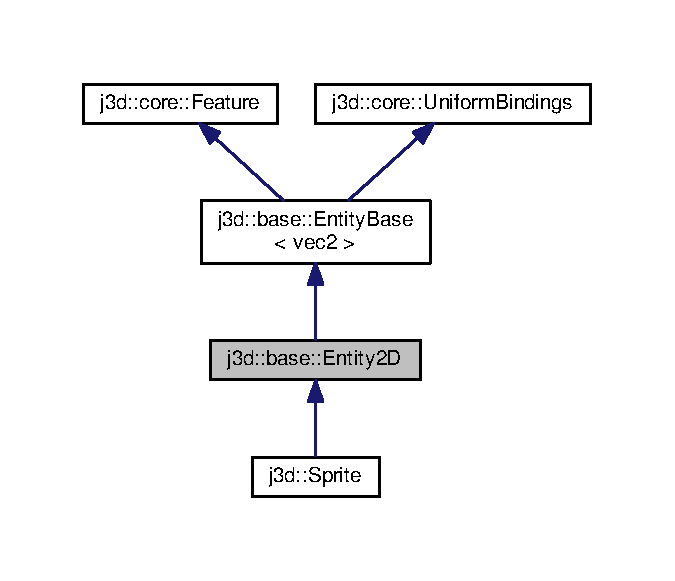
\includegraphics[width=324pt]{classj3d_1_1base_1_1Entity2D__inherit__graph}
\end{center}
\end{figure}


Collaboration diagram for j3d\+:\+:base\+:\+:Entity2\+D\+:
\nopagebreak
\begin{figure}[H]
\begin{center}
\leavevmode
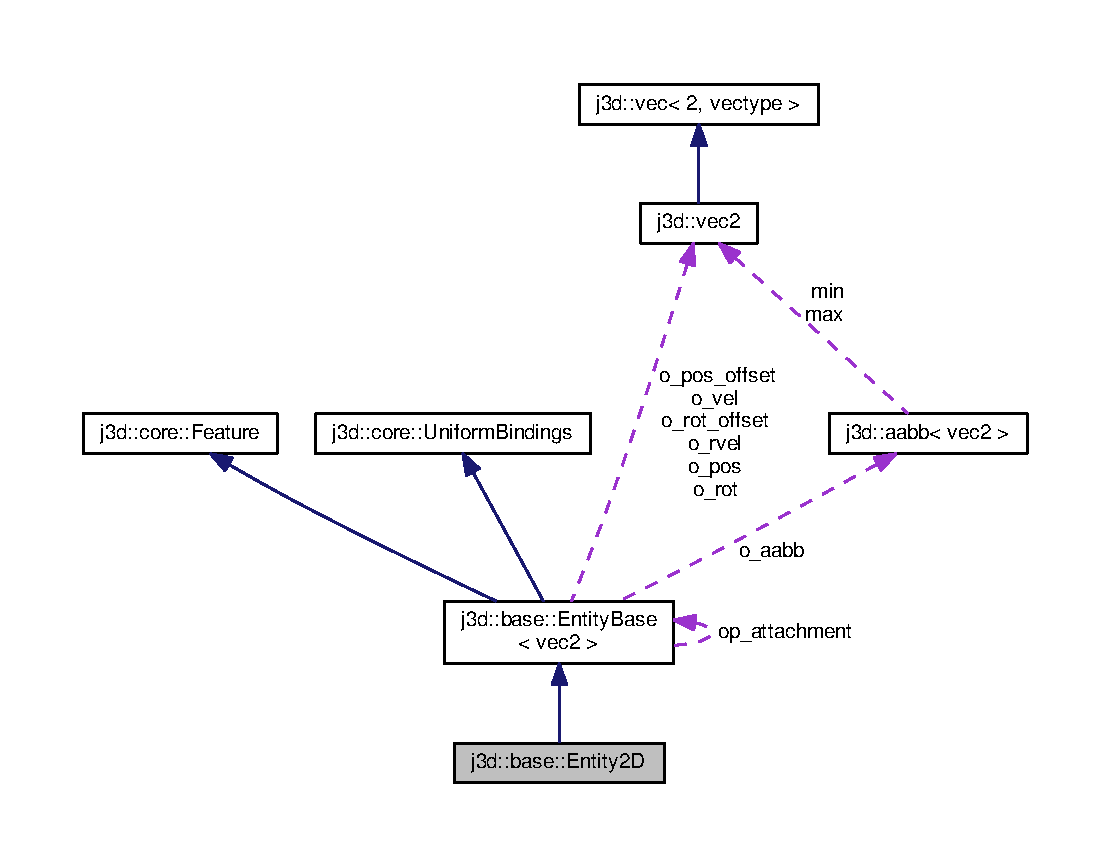
\includegraphics[width=350pt]{classj3d_1_1base_1_1Entity2D__coll__graph}
\end{center}
\end{figure}
\subsection*{Public Member Functions}
\begin{DoxyCompactItemize}
\item 
\hypertarget{classj3d_1_1base_1_1Entity2D_a52e01c12eec7f7fab6fdec3889e032e7}{}{\bfseries Entity2\+D} (string shader\+\_\+id)\label{classj3d_1_1base_1_1Entity2D_a52e01c12eec7f7fab6fdec3889e032e7}

\end{DoxyCompactItemize}
\subsection*{Additional Inherited Members}


The documentation for this class was generated from the following files\+:\begin{DoxyCompactItemize}
\item 
/media/will/ratchet/\+Projects/\+J\+A\+W/j3d-\/demo/j3d/base/entity\+\_\+2d.\+h\item 
/media/will/ratchet/\+Projects/\+J\+A\+W/j3d-\/demo/j3d/base/entity\+\_\+2d.\+cpp\end{DoxyCompactItemize}

\hypertarget{classj3d_1_1base_1_1EntityBase}{}\section{j3d\+:\+:base\+:\+:Entity\+Base$<$ T $>$ Class Template Reference}
\label{classj3d_1_1base_1_1EntityBase}\index{j3d\+::base\+::\+Entity\+Base$<$ T $>$@{j3d\+::base\+::\+Entity\+Base$<$ T $>$}}


Inheritance diagram for j3d\+:\+:base\+:\+:Entity\+Base$<$ T $>$\+:
\nopagebreak
\begin{figure}[H]
\begin{center}
\leavevmode
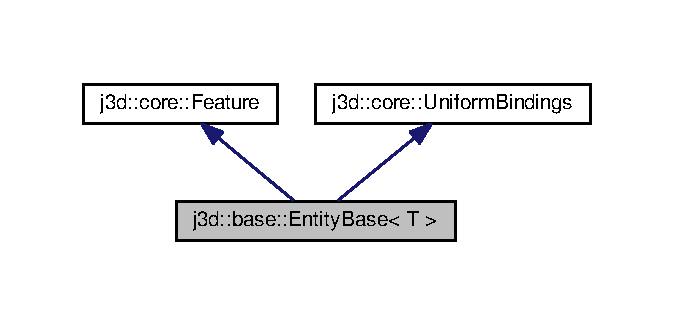
\includegraphics[width=324pt]{classj3d_1_1base_1_1EntityBase__inherit__graph}
\end{center}
\end{figure}


Collaboration diagram for j3d\+:\+:base\+:\+:Entity\+Base$<$ T $>$\+:
\nopagebreak
\begin{figure}[H]
\begin{center}
\leavevmode
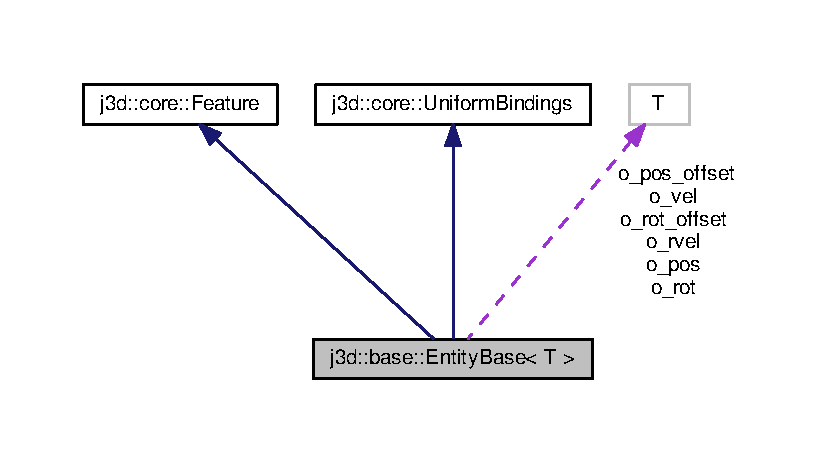
\includegraphics[width=350pt]{classj3d_1_1base_1_1EntityBase__coll__graph}
\end{center}
\end{figure}
\subsection*{Public Member Functions}
\begin{DoxyCompactItemize}
\item 
\hypertarget{classj3d_1_1base_1_1EntityBase_a306d0595cbccf6b497f39663e7bbf67d}{}{\bfseries Entity\+Base} (string shader\+\_\+id)\label{classj3d_1_1base_1_1EntityBase_a306d0595cbccf6b497f39663e7bbf67d}

\item 
\hypertarget{classj3d_1_1base_1_1EntityBase_a11ef641982250f6816b7c8276ec1e498}{}virtual void {\bfseries update} ()\label{classj3d_1_1base_1_1EntityBase_a11ef641982250f6816b7c8276ec1e498}

\item 
\hypertarget{classj3d_1_1base_1_1EntityBase_abfb3b9a7b986ffa5fef9429c71d7f653}{}virtual void {\bfseries spatialize} ()\label{classj3d_1_1base_1_1EntityBase_abfb3b9a7b986ffa5fef9429c71d7f653}

\item 
\hypertarget{classj3d_1_1base_1_1EntityBase_aaee6e91a90fa2099fbb30ee0817043a0}{}virtual void {\bfseries sync\+Attachment} ()\label{classj3d_1_1base_1_1EntityBase_aaee6e91a90fa2099fbb30ee0817043a0}

\item 
\hypertarget{classj3d_1_1base_1_1EntityBase_a1e109456587ef8dc4730ebdc2cb382c0}{}virtual \hyperlink{classj3d_1_1base_1_1EntityBase}{Entity\+Base}$<$ T $>$ $\ast$ {\bfseries move} (const T \&t)\label{classj3d_1_1base_1_1EntityBase_a1e109456587ef8dc4730ebdc2cb382c0}

\item 
\hypertarget{classj3d_1_1base_1_1EntityBase_a1735e8350927e7c4212dea37998433ee}{}virtual \hyperlink{classj3d_1_1base_1_1EntityBase}{Entity\+Base}$<$ T $>$ $\ast$ {\bfseries rotate} (const T \&t)\label{classj3d_1_1base_1_1EntityBase_a1735e8350927e7c4212dea37998433ee}

\item 
\hypertarget{classj3d_1_1base_1_1EntityBase_ae6fd806e59400c62c6e2bd17e8827ab6}{}virtual \hyperlink{classj3d_1_1base_1_1EntityBase}{Entity\+Base}$<$ T $>$ $\ast$ {\bfseries lock} (bool b=true)\label{classj3d_1_1base_1_1EntityBase_ae6fd806e59400c62c6e2bd17e8827ab6}

\item 
\hypertarget{classj3d_1_1base_1_1EntityBase_aa3c03efb213e8afceaba808463926bea}{}virtual \hyperlink{classj3d_1_1base_1_1EntityBase}{Entity\+Base}$<$ T $>$ $\ast$ {\bfseries pos} (const T \&t)\label{classj3d_1_1base_1_1EntityBase_aa3c03efb213e8afceaba808463926bea}

\item 
\hypertarget{classj3d_1_1base_1_1EntityBase_a755f372ef87b7491503cf7508c689acb}{}virtual \hyperlink{classj3d_1_1base_1_1EntityBase}{Entity\+Base}$<$ T $>$ $\ast$ {\bfseries rot} (const T \&t)\label{classj3d_1_1base_1_1EntityBase_a755f372ef87b7491503cf7508c689acb}

\item 
\hypertarget{classj3d_1_1base_1_1EntityBase_aab74f2504156f927a30d12483b9f1bc6}{}virtual \hyperlink{classj3d_1_1base_1_1EntityBase}{Entity\+Base}$<$ T $>$ $\ast$ {\bfseries vel} (const T \&t)\label{classj3d_1_1base_1_1EntityBase_aab74f2504156f927a30d12483b9f1bc6}

\item 
\hypertarget{classj3d_1_1base_1_1EntityBase_a9c4db4d13b9a894ce5b58fe42a4ee8e3}{}virtual \hyperlink{classj3d_1_1base_1_1EntityBase}{Entity\+Base}$<$ T $>$ $\ast$ {\bfseries rvel} (const T \&t)\label{classj3d_1_1base_1_1EntityBase_a9c4db4d13b9a894ce5b58fe42a4ee8e3}

\item 
\hypertarget{classj3d_1_1base_1_1EntityBase_a9928cc02583f5459adccb4fa77bbd969}{}virtual \hyperlink{classj3d_1_1base_1_1EntityBase}{Entity\+Base}$<$ T $>$ $\ast$ {\bfseries attach} (\hyperlink{classj3d_1_1base_1_1EntityBase}{Entity\+Base}$<$ T $>$ $\ast$ent, const T \&p, const T \&r)\label{classj3d_1_1base_1_1EntityBase_a9928cc02583f5459adccb4fa77bbd969}

\item 
\hypertarget{classj3d_1_1base_1_1EntityBase_a2062bc3ecc6dab95202f14987bcb3727}{}virtual \hyperlink{classj3d_1_1base_1_1EntityBase}{Entity\+Base}$<$ T $>$ $\ast$ {\bfseries aabb} (const T \&max)\label{classj3d_1_1base_1_1EntityBase_a2062bc3ecc6dab95202f14987bcb3727}

\item 
\hypertarget{classj3d_1_1base_1_1EntityBase_aac195b713d925cdac6faabc0260901a5}{}virtual \hyperlink{classj3d_1_1base_1_1EntityBase}{Entity\+Base}$<$ T $>$ $\ast$ {\bfseries aabb} (const T \&min, const T \&max)\label{classj3d_1_1base_1_1EntityBase_aac195b713d925cdac6faabc0260901a5}

\item 
\hypertarget{classj3d_1_1base_1_1EntityBase_a09879cf2b3b04d2e85cffb242c23aa60}{}virtual bool {\bfseries locked} () const \label{classj3d_1_1base_1_1EntityBase_a09879cf2b3b04d2e85cffb242c23aa60}

\item 
\hypertarget{classj3d_1_1base_1_1EntityBase_a9d2db3a52dcd08b24d2f39430396cd68}{}virtual const T \& {\bfseries pos} () const \label{classj3d_1_1base_1_1EntityBase_a9d2db3a52dcd08b24d2f39430396cd68}

\item 
\hypertarget{classj3d_1_1base_1_1EntityBase_ab68dd233c4d02cfced0760e0a6a7a83e}{}virtual const T \& {\bfseries rot} () const \label{classj3d_1_1base_1_1EntityBase_ab68dd233c4d02cfced0760e0a6a7a83e}

\item 
\hypertarget{classj3d_1_1base_1_1EntityBase_a9910fb25b949d01c335b81f3969d1df1}{}virtual const T \& {\bfseries vel} () const \label{classj3d_1_1base_1_1EntityBase_a9910fb25b949d01c335b81f3969d1df1}

\item 
\hypertarget{classj3d_1_1base_1_1EntityBase_ac0147f900e5b9d7f10be7a4b679a5e5b}{}virtual const T \& {\bfseries rvel} () const \label{classj3d_1_1base_1_1EntityBase_ac0147f900e5b9d7f10be7a4b679a5e5b}

\item 
\hypertarget{classj3d_1_1base_1_1EntityBase_a954552aeff368c1aea5a18fa38c0c1f2}{}virtual bool {\bfseries attached} () const \label{classj3d_1_1base_1_1EntityBase_a954552aeff368c1aea5a18fa38c0c1f2}

\item 
\hypertarget{classj3d_1_1base_1_1EntityBase_a6dbc6dcf2b3250235afbe4e501a3033b}{}virtual \hyperlink{classj3d_1_1base_1_1EntityBase}{Entity\+Base}$<$ T $>$ $\ast$ {\bfseries attachment} () const \label{classj3d_1_1base_1_1EntityBase_a6dbc6dcf2b3250235afbe4e501a3033b}

\item 
\hypertarget{classj3d_1_1base_1_1EntityBase_a9f57935d761f3d1ad63958bb955a1ff1}{}virtual void {\bfseries aabb} (\hyperlink{structj3d_1_1aabb}{j3d\+::aabb}$<$ T $>$ $\ast$out) const \label{classj3d_1_1base_1_1EntityBase_a9f57935d761f3d1ad63958bb955a1ff1}

\item 
\hypertarget{classj3d_1_1base_1_1EntityBase_a1105220b68436ee866b18e33dd4165b5}{}virtual \hyperlink{structj3d_1_1aabb}{j3d\+::aabb}$<$ T $>$ {\bfseries aabb} () const \label{classj3d_1_1base_1_1EntityBase_a1105220b68436ee866b18e33dd4165b5}

\end{DoxyCompactItemize}
\subsection*{Protected Attributes}
\begin{DoxyCompactItemize}
\item 
\hypertarget{classj3d_1_1base_1_1EntityBase_a723edac1cab8a39ed6153083bcd7487a}{}bool {\bfseries o\+\_\+locked}\label{classj3d_1_1base_1_1EntityBase_a723edac1cab8a39ed6153083bcd7487a}

\item 
\hypertarget{classj3d_1_1base_1_1EntityBase_aef5a3d9cf153970566a70ba3e868abdf}{}T {\bfseries o\+\_\+pos}\label{classj3d_1_1base_1_1EntityBase_aef5a3d9cf153970566a70ba3e868abdf}

\item 
\hypertarget{classj3d_1_1base_1_1EntityBase_aa3a47146742e4987e9e953ef4254908c}{}T {\bfseries o\+\_\+rot}\label{classj3d_1_1base_1_1EntityBase_aa3a47146742e4987e9e953ef4254908c}

\item 
\hypertarget{classj3d_1_1base_1_1EntityBase_ad759e3f7384e81593a062ebdbf4c8c69}{}T {\bfseries o\+\_\+pos\+\_\+offset}\label{classj3d_1_1base_1_1EntityBase_ad759e3f7384e81593a062ebdbf4c8c69}

\item 
\hypertarget{classj3d_1_1base_1_1EntityBase_aa31c9ae69db9516aef5fa41da0bbe634}{}T {\bfseries o\+\_\+rot\+\_\+offset}\label{classj3d_1_1base_1_1EntityBase_aa31c9ae69db9516aef5fa41da0bbe634}

\item 
\hypertarget{classj3d_1_1base_1_1EntityBase_ae99945875d6372e31b382100dd18a062}{}T {\bfseries o\+\_\+vel}\label{classj3d_1_1base_1_1EntityBase_ae99945875d6372e31b382100dd18a062}

\item 
\hypertarget{classj3d_1_1base_1_1EntityBase_a5139395dc5211ed7cc8fa20e9dd04da5}{}T {\bfseries o\+\_\+rvel}\label{classj3d_1_1base_1_1EntityBase_a5139395dc5211ed7cc8fa20e9dd04da5}

\item 
\hypertarget{classj3d_1_1base_1_1EntityBase_a545d6c77f50e1a8ea19fd3c0e47b0f3f}{}\hyperlink{classj3d_1_1base_1_1EntityBase}{Entity\+Base}$<$ T $>$ $\ast$ {\bfseries op\+\_\+attachment}\label{classj3d_1_1base_1_1EntityBase_a545d6c77f50e1a8ea19fd3c0e47b0f3f}

\item 
\hypertarget{classj3d_1_1base_1_1EntityBase_a98b4fee804003d891318c36f42838a00}{}\hyperlink{structj3d_1_1aabb}{j3d\+::aabb}$<$ T $>$ {\bfseries o\+\_\+aabb}\label{classj3d_1_1base_1_1EntityBase_a98b4fee804003d891318c36f42838a00}

\end{DoxyCompactItemize}


The documentation for this class was generated from the following file\+:\begin{DoxyCompactItemize}
\item 
/media/will/ratchet/\+Projects/\+J\+A\+W/j3d-\/demo/j3d/base/entity\+\_\+base.\+h\end{DoxyCompactItemize}

\hypertarget{classj3d_1_1core_1_1Feature}{}\section{j3d\+:\+:core\+:\+:Feature Class Reference}
\label{classj3d_1_1core_1_1Feature}\index{j3d\+::core\+::\+Feature@{j3d\+::core\+::\+Feature}}


Inheritance diagram for j3d\+:\+:core\+:\+:Feature\+:
\nopagebreak
\begin{figure}[H]
\begin{center}
\leavevmode
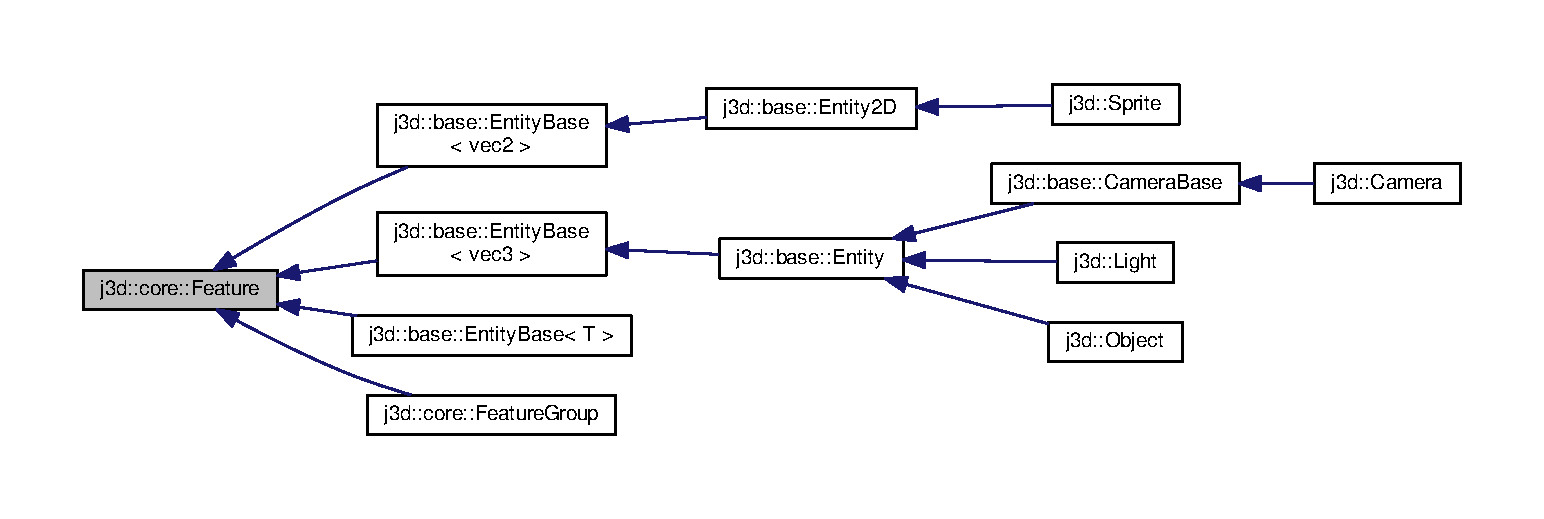
\includegraphics[width=350pt]{classj3d_1_1core_1_1Feature__inherit__graph}
\end{center}
\end{figure}
\subsection*{Public Member Functions}
\begin{DoxyCompactItemize}
\item 
\hypertarget{classj3d_1_1core_1_1Feature_a50b34b8e0ea2efaf582baf3effd9f4a8}{}virtual void {\bfseries update} ()\label{classj3d_1_1core_1_1Feature_a50b34b8e0ea2efaf582baf3effd9f4a8}

\item 
\hypertarget{classj3d_1_1core_1_1Feature_a93803d5262dea61d6def23e4351f3be1}{}virtual void {\bfseries render} ()\label{classj3d_1_1core_1_1Feature_a93803d5262dea61d6def23e4351f3be1}

\item 
\hypertarget{classj3d_1_1core_1_1Feature_a097dea6a9545ad5e79d360286f17ff72}{}bool {\bfseries grouped} () const \label{classj3d_1_1core_1_1Feature_a097dea6a9545ad5e79d360286f17ff72}

\item 
\hypertarget{classj3d_1_1core_1_1Feature_a0e9554c37fa23c1482d85e1ee648470f}{}\hyperlink{classj3d_1_1core_1_1Group}{Group} $\ast$ {\bfseries group} () const \label{classj3d_1_1core_1_1Feature_a0e9554c37fa23c1482d85e1ee648470f}

\end{DoxyCompactItemize}
\subsection*{Friends}
\begin{DoxyCompactItemize}
\item 
\hypertarget{classj3d_1_1core_1_1Feature_a2697825715974a353728f0d4d5658112}{}class {\bfseries Group}\label{classj3d_1_1core_1_1Feature_a2697825715974a353728f0d4d5658112}

\end{DoxyCompactItemize}


The documentation for this class was generated from the following file\+:\begin{DoxyCompactItemize}
\item 
/media/will/ratchet/\+Projects/\+J\+A\+W/j3d-\/demo/j3d/core/feature.\+h\end{DoxyCompactItemize}

\hypertarget{classj3d_1_1core_1_1FeatureGroup}{}\section{j3d\+:\+:core\+:\+:Feature\+Group Class Reference}
\label{classj3d_1_1core_1_1FeatureGroup}\index{j3d\+::core\+::\+Feature\+Group@{j3d\+::core\+::\+Feature\+Group}}


Inheritance diagram for j3d\+:\+:core\+:\+:Feature\+Group\+:
\nopagebreak
\begin{figure}[H]
\begin{center}
\leavevmode
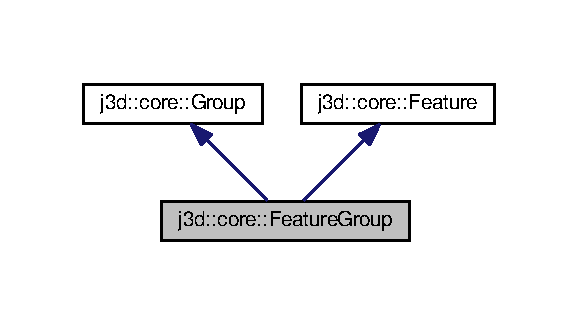
\includegraphics[width=278pt]{classj3d_1_1core_1_1FeatureGroup__inherit__graph}
\end{center}
\end{figure}


Collaboration diagram for j3d\+:\+:core\+:\+:Feature\+Group\+:
\nopagebreak
\begin{figure}[H]
\begin{center}
\leavevmode
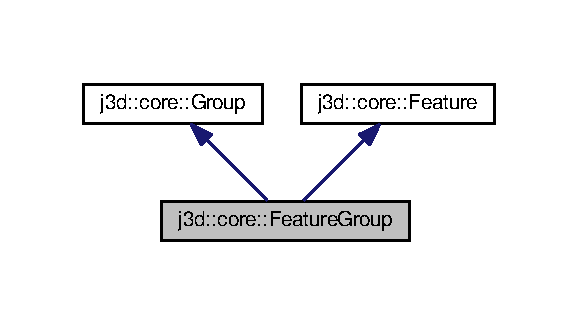
\includegraphics[width=278pt]{classj3d_1_1core_1_1FeatureGroup__coll__graph}
\end{center}
\end{figure}
\subsection*{Public Member Functions}
\begin{DoxyCompactItemize}
\item 
\hypertarget{classj3d_1_1core_1_1FeatureGroup_a7dd8a4f38351ec73140d1879bb43e1cf}{}{\bfseries Feature\+Group} (bool control\+\_\+delete=false)\label{classj3d_1_1core_1_1FeatureGroup_a7dd8a4f38351ec73140d1879bb43e1cf}

\end{DoxyCompactItemize}
\subsection*{Additional Inherited Members}


The documentation for this class was generated from the following file\+:\begin{DoxyCompactItemize}
\item 
/media/will/ratchet/\+Projects/\+J\+A\+W/j3d-\/demo/j3d/core/group.\+h\end{DoxyCompactItemize}

\hypertarget{classj3d_1_1core_1_1Flaggable}{}\section{j3d\+:\+:core\+:\+:Flaggable Class Reference}
\label{classj3d_1_1core_1_1Flaggable}\index{j3d\+::core\+::\+Flaggable@{j3d\+::core\+::\+Flaggable}}
\subsection*{Public Member Functions}
\begin{DoxyCompactItemize}
\item 
\hypertarget{classj3d_1_1core_1_1Flaggable_ae10da546e766dac4768bcd1d95309026}{}{\bfseries Flaggable} (uint64\+\_\+t start\+\_\+flags=0x0)\label{classj3d_1_1core_1_1Flaggable_ae10da546e766dac4768bcd1d95309026}

\item 
\hypertarget{classj3d_1_1core_1_1Flaggable_a003e21aa046dd59f4f572e57d52df84a}{}void {\bfseries flag} (uint64\+\_\+t f)\label{classj3d_1_1core_1_1Flaggable_a003e21aa046dd59f4f572e57d52df84a}

\item 
\hypertarget{classj3d_1_1core_1_1Flaggable_a45cfd6ad5aa5c9b1b2c1aaf916e4dbe8}{}void {\bfseries unflag} (uint64\+\_\+t f)\label{classj3d_1_1core_1_1Flaggable_a45cfd6ad5aa5c9b1b2c1aaf916e4dbe8}

\item 
\hypertarget{classj3d_1_1core_1_1Flaggable_a9d017d22ca4b29ea9fd5561e757916a5}{}void {\bfseries noflags} ()\label{classj3d_1_1core_1_1Flaggable_a9d017d22ca4b29ea9fd5561e757916a5}

\item 
\hypertarget{classj3d_1_1core_1_1Flaggable_aeadf0a69b8a228a8be7b860ba021ab8b}{}bool {\bfseries flagged} (uint64\+\_\+t f)\label{classj3d_1_1core_1_1Flaggable_aeadf0a69b8a228a8be7b860ba021ab8b}

\item 
\hypertarget{classj3d_1_1core_1_1Flaggable_a6272023846e3dcafc11299f6aadced96}{}bool {\bfseries unflagged} (uint64\+\_\+t f)\label{classj3d_1_1core_1_1Flaggable_a6272023846e3dcafc11299f6aadced96}

\item 
\hypertarget{classj3d_1_1core_1_1Flaggable_a2f69054e94b4e0d2c876dc68dc1a6ad4}{}uint64\+\_\+t {\bfseries flags} ()\label{classj3d_1_1core_1_1Flaggable_a2f69054e94b4e0d2c876dc68dc1a6ad4}

\end{DoxyCompactItemize}
\subsection*{Protected Attributes}
\begin{DoxyCompactItemize}
\item 
\hypertarget{classj3d_1_1core_1_1Flaggable_a933c2b776cf24091b0eee6c836f57f7a}{}uint64\+\_\+t {\bfseries o\+\_\+flags}\label{classj3d_1_1core_1_1Flaggable_a933c2b776cf24091b0eee6c836f57f7a}

\end{DoxyCompactItemize}


The documentation for this class was generated from the following files\+:\begin{DoxyCompactItemize}
\item 
/media/will/ratchet/\+Projects/\+J\+A\+W/j3d-\/demo/j3d/core/flaggable.\+h\item 
/media/will/ratchet/\+Projects/\+J\+A\+W/j3d-\/demo/j3d/core/flaggable.\+cpp\end{DoxyCompactItemize}

\hypertarget{classj3d_1_1FloorMesh}{}\section{j3d\+:\+:Floor\+Mesh Class Reference}
\label{classj3d_1_1FloorMesh}\index{j3d\+::\+Floor\+Mesh@{j3d\+::\+Floor\+Mesh}}


Inheritance diagram for j3d\+:\+:Floor\+Mesh\+:
\nopagebreak
\begin{figure}[H]
\begin{center}
\leavevmode
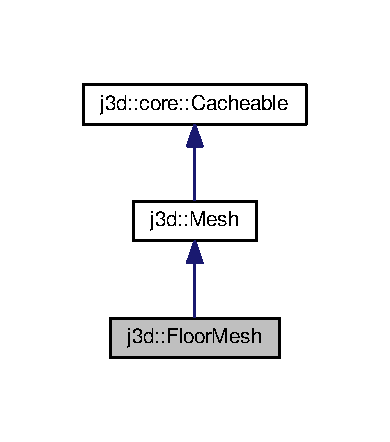
\includegraphics[width=187pt]{classj3d_1_1FloorMesh__inherit__graph}
\end{center}
\end{figure}


Collaboration diagram for j3d\+:\+:Floor\+Mesh\+:
\nopagebreak
\begin{figure}[H]
\begin{center}
\leavevmode
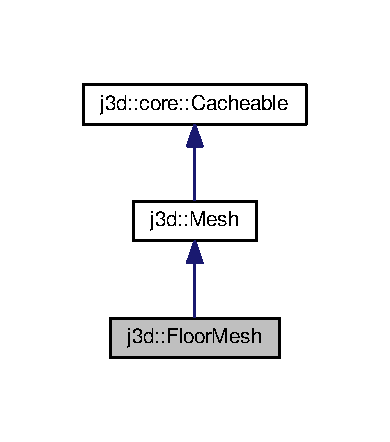
\includegraphics[width=187pt]{classj3d_1_1FloorMesh__coll__graph}
\end{center}
\end{figure}
\subsection*{Public Member Functions}
\begin{DoxyCompactItemize}
\item 
\hypertarget{classj3d_1_1FloorMesh_a6fedbd345f7b9e35c31dacfdb5d7ad06}{}{\bfseries Floor\+Mesh} (const char $\ast$id, float w, float l=0)\label{classj3d_1_1FloorMesh_a6fedbd345f7b9e35c31dacfdb5d7ad06}

\item 
\hypertarget{classj3d_1_1FloorMesh_a1af3571a2f3b2bd06d7d6170a66052a6}{}float {\bfseries width} () const \label{classj3d_1_1FloorMesh_a1af3571a2f3b2bd06d7d6170a66052a6}

\item 
\hypertarget{classj3d_1_1FloorMesh_aa47a3ce7815913cbc107ddf0a6073668}{}float {\bfseries length} () const \label{classj3d_1_1FloorMesh_aa47a3ce7815913cbc107ddf0a6073668}

\end{DoxyCompactItemize}
\subsection*{Additional Inherited Members}


The documentation for this class was generated from the following files\+:\begin{DoxyCompactItemize}
\item 
/media/will/ratchet/\+Projects/\+J\+A\+W/j3d-\/demo/j3d/mesh\+\_\+shapes.\+h\item 
/media/will/ratchet/\+Projects/\+J\+A\+W/j3d-\/demo/j3d/mesh\+\_\+shapes.\+cpp\end{DoxyCompactItemize}

\hypertarget{classj3d_1_1util_1_1fps}{}\section{j3d\+:\+:util\+:\+:fps Class Reference}
\label{classj3d_1_1util_1_1fps}\index{j3d\+::util\+::fps@{j3d\+::util\+::fps}}
\subsection*{Static Public Member Functions}
\begin{DoxyCompactItemize}
\item 
\hypertarget{classj3d_1_1util_1_1fps_a3e6ec087e902a285d8e11dc9e98b08c4}{}static void {\bfseries enable} (bool b=true)\label{classj3d_1_1util_1_1fps_a3e6ec087e902a285d8e11dc9e98b08c4}

\item 
\hypertarget{classj3d_1_1util_1_1fps_a4ff846ef6ca1937a996cb80b71bffd9a}{}static void {\bfseries disable} (bool b=true)\label{classj3d_1_1util_1_1fps_a4ff846ef6ca1937a996cb80b71bffd9a}

\item 
\hypertarget{classj3d_1_1util_1_1fps_a5c8e3452aac20cf37cf05e2c6b862605}{}static void {\bfseries lap} (float)\label{classj3d_1_1util_1_1fps_a5c8e3452aac20cf37cf05e2c6b862605}

\item 
\hypertarget{classj3d_1_1util_1_1fps_a039721c0351b560734e3caab3128739f}{}static bool {\bfseries enabled} ()\label{classj3d_1_1util_1_1fps_a039721c0351b560734e3caab3128739f}

\item 
\hypertarget{classj3d_1_1util_1_1fps_a721fd529d88ece684caed8a3a37426cc}{}static unsigned int {\bfseries latest} ()\label{classj3d_1_1util_1_1fps_a721fd529d88ece684caed8a3a37426cc}

\item 
\hypertarget{classj3d_1_1util_1_1fps_a64311f5e08d4889ccc6b73219fee0101}{}static float {\bfseries lap} ()\label{classj3d_1_1util_1_1fps_a64311f5e08d4889ccc6b73219fee0101}

\item 
\hypertarget{classj3d_1_1util_1_1fps_a2a3a28930241574cf4db318d8ebc7ced}{}static bool {\bfseries notify} ()\label{classj3d_1_1util_1_1fps_a2a3a28930241574cf4db318d8ebc7ced}

\end{DoxyCompactItemize}
\subsection*{Friends}
\begin{DoxyCompactItemize}
\item 
\hypertarget{classj3d_1_1util_1_1fps_ad31738c6e067e2d37a806cefad63155c}{}class {\bfseries cycle}\label{classj3d_1_1util_1_1fps_ad31738c6e067e2d37a806cefad63155c}

\end{DoxyCompactItemize}


The documentation for this class was generated from the following files\+:\begin{DoxyCompactItemize}
\item 
/media/will/ratchet/\+Projects/\+J\+A\+W/j3d-\/demo/j3d/util/util.\+h\item 
/media/will/ratchet/\+Projects/\+J\+A\+W/j3d-\/demo/j3d/util/util.\+cpp\end{DoxyCompactItemize}

\hypertarget{classj3d_1_1ShaderProgram_1_1FragmentShader}{}\section{j3d\+:\+:Shader\+Program\+:\+:Fragment\+Shader Class Reference}
\label{classj3d_1_1ShaderProgram_1_1FragmentShader}\index{j3d\+::\+Shader\+Program\+::\+Fragment\+Shader@{j3d\+::\+Shader\+Program\+::\+Fragment\+Shader}}


Inheritance diagram for j3d\+:\+:Shader\+Program\+:\+:Fragment\+Shader\+:
\nopagebreak
\begin{figure}[H]
\begin{center}
\leavevmode
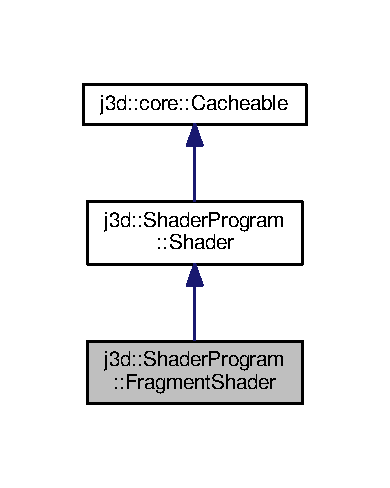
\includegraphics[width=187pt]{classj3d_1_1ShaderProgram_1_1FragmentShader__inherit__graph}
\end{center}
\end{figure}


Collaboration diagram for j3d\+:\+:Shader\+Program\+:\+:Fragment\+Shader\+:
\nopagebreak
\begin{figure}[H]
\begin{center}
\leavevmode
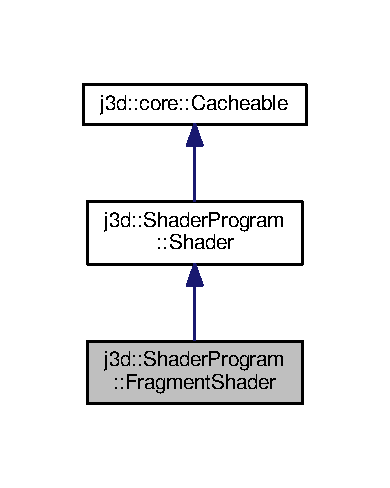
\includegraphics[width=187pt]{classj3d_1_1ShaderProgram_1_1FragmentShader__coll__graph}
\end{center}
\end{figure}
\subsection*{Public Member Functions}
\begin{DoxyCompactItemize}
\item 
\hypertarget{classj3d_1_1ShaderProgram_1_1FragmentShader_a7f94ca0e3a5d5f5662be4f9bb3bf01a9}{}{\bfseries Fragment\+Shader} (const char $\ast$path)\label{classj3d_1_1ShaderProgram_1_1FragmentShader_a7f94ca0e3a5d5f5662be4f9bb3bf01a9}

\end{DoxyCompactItemize}
\subsection*{Additional Inherited Members}


The documentation for this class was generated from the following file\+:\begin{DoxyCompactItemize}
\item 
/media/will/ratchet/\+Projects/\+J\+A\+W/j3d-\/demo/j3d/shader.\+h\end{DoxyCompactItemize}

\hypertarget{classj3d_1_1core_1_1Group}{}\section{j3d\+:\+:core\+:\+:Group Class Reference}
\label{classj3d_1_1core_1_1Group}\index{j3d\+::core\+::\+Group@{j3d\+::core\+::\+Group}}


Inheritance diagram for j3d\+:\+:core\+:\+:Group\+:
\nopagebreak
\begin{figure}[H]
\begin{center}
\leavevmode
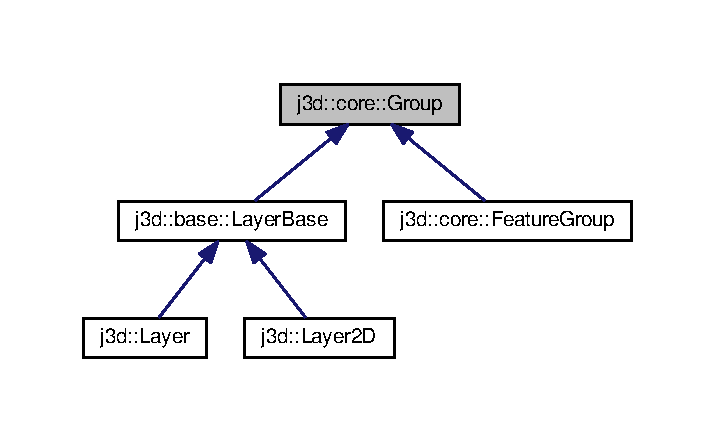
\includegraphics[width=343pt]{classj3d_1_1core_1_1Group__inherit__graph}
\end{center}
\end{figure}
\subsection*{Public Member Functions}
\begin{DoxyCompactItemize}
\item 
\hypertarget{classj3d_1_1core_1_1Group_aad98596f5fce0065e466aa8adecb9425}{}{\bfseries Group} (bool control\+\_\+delete=true)\label{classj3d_1_1core_1_1Group_aad98596f5fce0065e466aa8adecb9425}

\item 
\hypertarget{classj3d_1_1core_1_1Group_a821f3e0f7c9a896b907b4dbe069c7cb0}{}\hyperlink{classj3d_1_1core_1_1Group}{Group} $\ast$ {\bfseries group\+Add} (\hyperlink{classj3d_1_1core_1_1Feature}{Feature} $\ast$)\label{classj3d_1_1core_1_1Group_a821f3e0f7c9a896b907b4dbe069c7cb0}

\item 
\hypertarget{classj3d_1_1core_1_1Group_abcf63693db9788ec6ad1a576cb415ec4}{}\hyperlink{classj3d_1_1core_1_1Group}{Group} $\ast$ {\bfseries group\+Add} (initializer\+\_\+list$<$ \hyperlink{classj3d_1_1core_1_1Feature}{Feature} $\ast$ $>$)\label{classj3d_1_1core_1_1Group_abcf63693db9788ec6ad1a576cb415ec4}

\item 
\hypertarget{classj3d_1_1core_1_1Group_aff4d04686fc01797834c16002f3a7c79}{}\hyperlink{classj3d_1_1core_1_1Group}{Group} $\ast$ {\bfseries group\+Remove} (\hyperlink{classj3d_1_1core_1_1Feature}{Feature} $\ast$)\label{classj3d_1_1core_1_1Group_aff4d04686fc01797834c16002f3a7c79}

\item 
\hypertarget{classj3d_1_1core_1_1Group_afef85ea04b05cb9a774499608250624d}{}\hyperlink{classj3d_1_1core_1_1Group}{Group} $\ast$ {\bfseries group\+Remove} (initializer\+\_\+list$<$ \hyperlink{classj3d_1_1core_1_1Feature}{Feature} $\ast$ $>$)\label{classj3d_1_1core_1_1Group_afef85ea04b05cb9a774499608250624d}

\item 
\hypertarget{classj3d_1_1core_1_1Group_a97d8cfe41662dace45c6894ae632ddde}{}void {\bfseries group\+Delete} ()\label{classj3d_1_1core_1_1Group_a97d8cfe41662dace45c6894ae632ddde}

\item 
\hypertarget{classj3d_1_1core_1_1Group_ac6d787e9fcb2d11a519a122112b61cb4}{}virtual \hyperlink{classj3d_1_1core_1_1Group}{Group} $\ast$ {\bfseries add} (\hyperlink{classj3d_1_1core_1_1Feature}{Feature} $\ast$f)\label{classj3d_1_1core_1_1Group_ac6d787e9fcb2d11a519a122112b61cb4}

\item 
\hypertarget{classj3d_1_1core_1_1Group_a4187ed9f65745b701395199a541b3da7}{}virtual \hyperlink{classj3d_1_1core_1_1Group}{Group} $\ast$ {\bfseries add} (initializer\+\_\+list$<$ \hyperlink{classj3d_1_1core_1_1Feature}{Feature} $\ast$ $>$ fs)\label{classj3d_1_1core_1_1Group_a4187ed9f65745b701395199a541b3da7}

\item 
\hypertarget{classj3d_1_1core_1_1Group_aeb2c3ce4c025ee94525cfc68298c6cfb}{}virtual \hyperlink{classj3d_1_1core_1_1Group}{Group} $\ast$ {\bfseries remove} (\hyperlink{classj3d_1_1core_1_1Feature}{Feature} $\ast$f)\label{classj3d_1_1core_1_1Group_aeb2c3ce4c025ee94525cfc68298c6cfb}

\item 
\hypertarget{classj3d_1_1core_1_1Group_a5511f04521462b18cf40a889240c9825}{}virtual \hyperlink{classj3d_1_1core_1_1Group}{Group} $\ast$ {\bfseries remove} (initializer\+\_\+list$<$ \hyperlink{classj3d_1_1core_1_1Feature}{Feature} $\ast$ $>$ fs)\label{classj3d_1_1core_1_1Group_a5511f04521462b18cf40a889240c9825}

\item 
\hypertarget{classj3d_1_1core_1_1Group_ac0806ba745f20e6dfe8d0dea1202ba1e}{}void {\bfseries group\+Update} ()\label{classj3d_1_1core_1_1Group_ac0806ba745f20e6dfe8d0dea1202ba1e}

\item 
\hypertarget{classj3d_1_1core_1_1Group_a51cccc2b24c1d6754e736cc65dd57e17}{}void {\bfseries group\+Pre\+Render} ()\label{classj3d_1_1core_1_1Group_a51cccc2b24c1d6754e736cc65dd57e17}

\item 
\hypertarget{classj3d_1_1core_1_1Group_a990276b13134f0e2c4a397d62662b3e9}{}void {\bfseries group\+Render} ()\label{classj3d_1_1core_1_1Group_a990276b13134f0e2c4a397d62662b3e9}

\item 
\hypertarget{classj3d_1_1core_1_1Group_a18ec2927a002fc9cce22695b20b8f364}{}void {\bfseries group\+Post\+Render} ()\label{classj3d_1_1core_1_1Group_a18ec2927a002fc9cce22695b20b8f364}

\item 
\hypertarget{classj3d_1_1core_1_1Group_a530bd8fa97850845828916997bf471fa}{}void {\bfseries group\+Update\+Render} ()\label{classj3d_1_1core_1_1Group_a530bd8fa97850845828916997bf471fa}

\item 
\hypertarget{classj3d_1_1core_1_1Group_a64ad0f9b90512cead51e2ec404aa82b1}{}virtual void {\bfseries update} ()\label{classj3d_1_1core_1_1Group_a64ad0f9b90512cead51e2ec404aa82b1}

\item 
\hypertarget{classj3d_1_1core_1_1Group_a571dd5f2e388e3f24f877e90e28476a4}{}virtual void {\bfseries pre\+Render} ()\label{classj3d_1_1core_1_1Group_a571dd5f2e388e3f24f877e90e28476a4}

\item 
\hypertarget{classj3d_1_1core_1_1Group_ad13c52f186a2c3e5ba1af430077baf07}{}virtual void {\bfseries render} ()\label{classj3d_1_1core_1_1Group_ad13c52f186a2c3e5ba1af430077baf07}

\item 
\hypertarget{classj3d_1_1core_1_1Group_aa1f2ee4e7f6d7856c37600772db0a2d4}{}virtual void {\bfseries post\+Render} ()\label{classj3d_1_1core_1_1Group_aa1f2ee4e7f6d7856c37600772db0a2d4}

\item 
\hypertarget{classj3d_1_1core_1_1Group_afc06584a76c0036c09811d865db14b93}{}virtual void {\bfseries update\+Render} ()\label{classj3d_1_1core_1_1Group_afc06584a76c0036c09811d865db14b93}

\item 
\hypertarget{classj3d_1_1core_1_1Group_af3af0a862eb113000d338bacbd929208}{}\hyperlink{classj3d_1_1core_1_1Group}{Group} $\ast$ {\bfseries group\+Control\+Delete} (bool b=true)\label{classj3d_1_1core_1_1Group_af3af0a862eb113000d338bacbd929208}

\item 
\hypertarget{classj3d_1_1core_1_1Group_aabd996d4773b60ad51013850c33e3760}{}\hyperlink{classj3d_1_1core_1_1Group}{Group} $\ast$ {\bfseries group\+Shader\+Program} (const char $\ast$id)\label{classj3d_1_1core_1_1Group_aabd996d4773b60ad51013850c33e3760}

\item 
\hypertarget{classj3d_1_1core_1_1Group_a289bc7043a3e58629e12e0efd5e96abc}{}\hyperlink{classj3d_1_1core_1_1Group}{Group} $\ast$ {\bfseries group\+Shader\+Program} (\hyperlink{classj3d_1_1ShaderProgram}{Shader\+Program} $\ast$)\label{classj3d_1_1core_1_1Group_a289bc7043a3e58629e12e0efd5e96abc}

\item 
\hypertarget{classj3d_1_1core_1_1Group_aa28abf8f52dcde0472d15fecaae65bf4}{}virtual \hyperlink{classj3d_1_1core_1_1Group}{Group} $\ast$ {\bfseries control\+Delete} (bool b=true)\label{classj3d_1_1core_1_1Group_aa28abf8f52dcde0472d15fecaae65bf4}

\item 
\hypertarget{classj3d_1_1core_1_1Group_a1bb4f33e3b6d0bcffc08cd123a940bae}{}virtual \hyperlink{classj3d_1_1core_1_1Group}{Group} $\ast$ {\bfseries shader\+Program} (const char $\ast$id)\label{classj3d_1_1core_1_1Group_a1bb4f33e3b6d0bcffc08cd123a940bae}

\item 
\hypertarget{classj3d_1_1core_1_1Group_ac210250f090296d72f995babe4ce9cc5}{}virtual \hyperlink{classj3d_1_1core_1_1Group}{Group} $\ast$ {\bfseries shader\+Program} (\hyperlink{classj3d_1_1ShaderProgram}{Shader\+Program} $\ast$p)\label{classj3d_1_1core_1_1Group_ac210250f090296d72f995babe4ce9cc5}

\item 
\hypertarget{classj3d_1_1core_1_1Group_a0fac6844c447a8a2ebb63293c7db817d}{}bool {\bfseries group\+Control\+Delete} () const \label{classj3d_1_1core_1_1Group_a0fac6844c447a8a2ebb63293c7db817d}

\item 
\hypertarget{classj3d_1_1core_1_1Group_ad6449590d7a2ca67c5f0d63217a213ea}{}\hyperlink{classj3d_1_1ShaderProgram}{Shader\+Program} $\ast$ {\bfseries group\+Shader\+Program} () const \label{classj3d_1_1core_1_1Group_ad6449590d7a2ca67c5f0d63217a213ea}

\item 
\hypertarget{classj3d_1_1core_1_1Group_af8191deae7d090914af65aa35963fc7a}{}virtual bool {\bfseries control\+Delete} () const \label{classj3d_1_1core_1_1Group_af8191deae7d090914af65aa35963fc7a}

\item 
\hypertarget{classj3d_1_1core_1_1Group_af12b2ca247093cb2dce0eabe4c546aac}{}virtual \hyperlink{classj3d_1_1ShaderProgram}{Shader\+Program} $\ast$ {\bfseries shader\+Program} () const \label{classj3d_1_1core_1_1Group_af12b2ca247093cb2dce0eabe4c546aac}

\end{DoxyCompactItemize}
\subsection*{Protected Member Functions}
\begin{DoxyCompactItemize}
\item 
\hypertarget{classj3d_1_1core_1_1Group_aead6e49eb90b6f6d3811ac4ccfa5f1fa}{}virtual void {\bfseries on\+Group\+Add} (\hyperlink{classj3d_1_1core_1_1Feature}{Feature} $\ast$)\label{classj3d_1_1core_1_1Group_aead6e49eb90b6f6d3811ac4ccfa5f1fa}

\item 
\hypertarget{classj3d_1_1core_1_1Group_ab18fab54fbd0acebc63745c1a47c7a97}{}virtual void {\bfseries on\+Group\+Remove} (\hyperlink{classj3d_1_1core_1_1Feature}{Feature} $\ast$)\label{classj3d_1_1core_1_1Group_ab18fab54fbd0acebc63745c1a47c7a97}

\end{DoxyCompactItemize}
\subsection*{Protected Attributes}
\begin{DoxyCompactItemize}
\item 
\hypertarget{classj3d_1_1core_1_1Group_afb345d975b0a0e1c85f0b55bfe52bd70}{}unordered\+\_\+map$<$ string, \hyperlink{classj3d_1_1core_1_1Feature}{Feature} $\ast$ $>$ {\bfseries o\+\_\+features}\label{classj3d_1_1core_1_1Group_afb345d975b0a0e1c85f0b55bfe52bd70}

\item 
\hypertarget{classj3d_1_1core_1_1Group_acf9f16f1bf435fd55ef5e96e87598fc6}{}bool {\bfseries o\+\_\+pre\+\_\+render}\label{classj3d_1_1core_1_1Group_acf9f16f1bf435fd55ef5e96e87598fc6}

\end{DoxyCompactItemize}


The documentation for this class was generated from the following files\+:\begin{DoxyCompactItemize}
\item 
/media/will/ratchet/\+Projects/\+J\+A\+W/j3d-\/demo/j3d/core/group.\+h\item 
/media/will/ratchet/\+Projects/\+J\+A\+W/j3d-\/demo/j3d/core/group.\+cpp\end{DoxyCompactItemize}

\hypertarget{structj3d_1_1util_1_1is__pointer}{}\section{j3d\+:\+:util\+:\+:is\+\_\+pointer$<$ T $>$ Struct Template Reference}
\label{structj3d_1_1util_1_1is__pointer}\index{j3d\+::util\+::is\+\_\+pointer$<$ T $>$@{j3d\+::util\+::is\+\_\+pointer$<$ T $>$}}
\subsection*{Static Public Attributes}
\begin{DoxyCompactItemize}
\item 
\hypertarget{structj3d_1_1util_1_1is__pointer_a378ef0f6c020a72f7fef4d410f44e53a}{}static const bool {\bfseries value} = false\label{structj3d_1_1util_1_1is__pointer_a378ef0f6c020a72f7fef4d410f44e53a}

\end{DoxyCompactItemize}


The documentation for this struct was generated from the following file\+:\begin{DoxyCompactItemize}
\item 
/media/will/ratchet/\+Projects/\+J\+A\+W/j3d-\/demo/j3d/util/util.\+h\end{DoxyCompactItemize}

\hypertarget{structj3d_1_1util_1_1is__pointer_3_01T_01_5_01_4}{}\section{j3d\+:\+:util\+:\+:is\+\_\+pointer$<$ T $\ast$ $>$ Struct Template Reference}
\label{structj3d_1_1util_1_1is__pointer_3_01T_01_5_01_4}\index{j3d\+::util\+::is\+\_\+pointer$<$ T $\ast$ $>$@{j3d\+::util\+::is\+\_\+pointer$<$ T $\ast$ $>$}}
\subsection*{Static Public Attributes}
\begin{DoxyCompactItemize}
\item 
\hypertarget{structj3d_1_1util_1_1is__pointer_3_01T_01_5_01_4_ad4412846dd8d83bde541ac102f8be48c}{}static const bool {\bfseries value} = true\label{structj3d_1_1util_1_1is__pointer_3_01T_01_5_01_4_ad4412846dd8d83bde541ac102f8be48c}

\end{DoxyCompactItemize}


The documentation for this struct was generated from the following file\+:\begin{DoxyCompactItemize}
\item 
/media/will/ratchet/\+Projects/\+J\+A\+W/j3d-\/demo/j3d/util/util.\+h\end{DoxyCompactItemize}

\hypertarget{classj3d_1_1Layer}{}\section{j3d\+:\+:Layer Class Reference}
\label{classj3d_1_1Layer}\index{j3d\+::\+Layer@{j3d\+::\+Layer}}


Inheritance diagram for j3d\+:\+:Layer\+:
\nopagebreak
\begin{figure}[H]
\begin{center}
\leavevmode
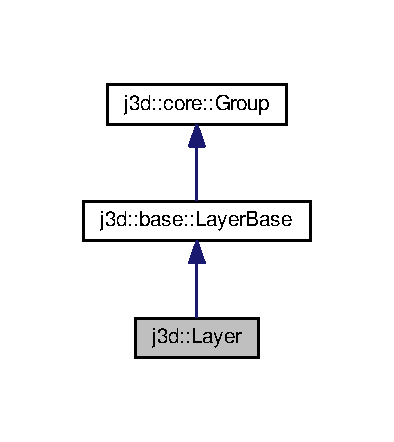
\includegraphics[width=189pt]{classj3d_1_1Layer__inherit__graph}
\end{center}
\end{figure}


Collaboration diagram for j3d\+:\+:Layer\+:
\nopagebreak
\begin{figure}[H]
\begin{center}
\leavevmode
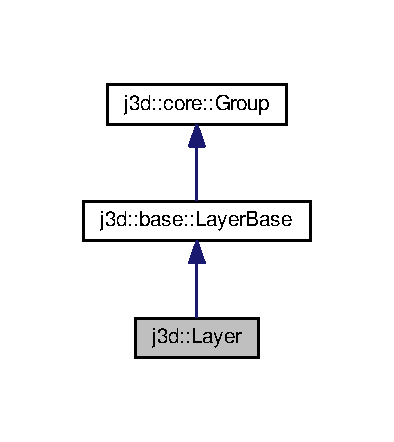
\includegraphics[width=189pt]{classj3d_1_1Layer__coll__graph}
\end{center}
\end{figure}
\subsection*{Public Member Functions}
\begin{DoxyCompactItemize}
\item 
\hypertarget{classj3d_1_1Layer_a4ee90be1500602909d319446877bf22f}{}{\bfseries Layer} (bool control\+\_\+delete=true)\label{classj3d_1_1Layer_a4ee90be1500602909d319446877bf22f}

\item 
\hypertarget{classj3d_1_1Layer_a7fe5312b9dd98f3cc1945cb31fd66efe}{}void {\bfseries render} ()\label{classj3d_1_1Layer_a7fe5312b9dd98f3cc1945cb31fd66efe}

\item 
\hypertarget{classj3d_1_1Layer_aa3f87e5f4c5739ab54e7ee6f7b2d907a}{}void {\bfseries update\+Render} ()\label{classj3d_1_1Layer_aa3f87e5f4c5739ab54e7ee6f7b2d907a}

\end{DoxyCompactItemize}
\subsection*{Protected Member Functions}
\begin{DoxyCompactItemize}
\item 
\hypertarget{classj3d_1_1Layer_a2c10403bbb9854522ccf606a161622d5}{}void {\bfseries on\+Group\+Add} (\hyperlink{classj3d_1_1core_1_1Feature}{core\+::\+Feature} $\ast$)\label{classj3d_1_1Layer_a2c10403bbb9854522ccf606a161622d5}

\end{DoxyCompactItemize}
\subsection*{Additional Inherited Members}


The documentation for this class was generated from the following files\+:\begin{DoxyCompactItemize}
\item 
/media/will/ratchet/\+Projects/\+J\+A\+W/j3d-\/demo/j3d/layer.\+h\item 
/media/will/ratchet/\+Projects/\+J\+A\+W/j3d-\/demo/j3d/layer.\+cpp\end{DoxyCompactItemize}

\hypertarget{classj3d_1_1Layer2D}{}\section{j3d\+:\+:Layer2\+D Class Reference}
\label{classj3d_1_1Layer2D}\index{j3d\+::\+Layer2\+D@{j3d\+::\+Layer2\+D}}


Inheritance diagram for j3d\+:\+:Layer2\+D\+:
\nopagebreak
\begin{figure}[H]
\begin{center}
\leavevmode
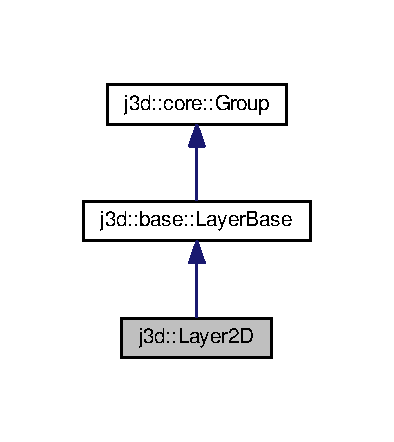
\includegraphics[width=189pt]{classj3d_1_1Layer2D__inherit__graph}
\end{center}
\end{figure}


Collaboration diagram for j3d\+:\+:Layer2\+D\+:
\nopagebreak
\begin{figure}[H]
\begin{center}
\leavevmode
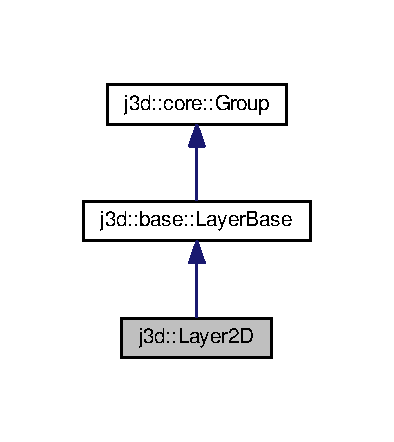
\includegraphics[width=189pt]{classj3d_1_1Layer2D__coll__graph}
\end{center}
\end{figure}
\subsection*{Public Member Functions}
\begin{DoxyCompactItemize}
\item 
\hypertarget{classj3d_1_1Layer2D_a6f9a278af6814d14162c85bc71f0daec}{}{\bfseries Layer2\+D} (bool control\+\_\+delete=true)\label{classj3d_1_1Layer2D_a6f9a278af6814d14162c85bc71f0daec}

\item 
\hypertarget{classj3d_1_1Layer2D_ae6999e2c08f1adee67ab904836bb563f}{}\hyperlink{classj3d_1_1Layer2D}{Layer2\+D} $\ast$ {\bfseries add} (\hyperlink{classj3d_1_1Sprite}{Sprite} $\ast$)\label{classj3d_1_1Layer2D_ae6999e2c08f1adee67ab904836bb563f}

\item 
\hypertarget{classj3d_1_1Layer2D_a3172565d286e5978c35bf29a6919d483}{}\hyperlink{classj3d_1_1Layer2D}{Layer2\+D} $\ast$ {\bfseries add} (initializer\+\_\+list$<$ \hyperlink{classj3d_1_1Sprite}{Sprite} $\ast$ $>$)\label{classj3d_1_1Layer2D_a3172565d286e5978c35bf29a6919d483}

\end{DoxyCompactItemize}
\subsection*{Additional Inherited Members}


The documentation for this class was generated from the following files\+:\begin{DoxyCompactItemize}
\item 
/media/will/ratchet/\+Projects/\+J\+A\+W/j3d-\/demo/j3d/layer\+\_\+2d.\+h\item 
/media/will/ratchet/\+Projects/\+J\+A\+W/j3d-\/demo/j3d/layer\+\_\+2d.\+cpp\end{DoxyCompactItemize}

\hypertarget{classj3d_1_1base_1_1LayerBase}{}\section{j3d\+:\+:base\+:\+:Layer\+Base Class Reference}
\label{classj3d_1_1base_1_1LayerBase}\index{j3d\+::base\+::\+Layer\+Base@{j3d\+::base\+::\+Layer\+Base}}


Inheritance diagram for j3d\+:\+:base\+:\+:Layer\+Base\+:
\nopagebreak
\begin{figure}[H]
\begin{center}
\leavevmode
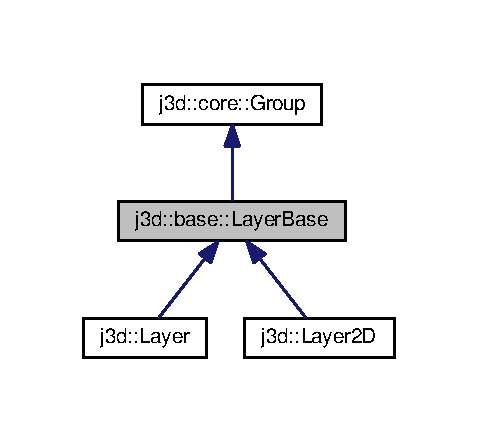
\includegraphics[width=230pt]{classj3d_1_1base_1_1LayerBase__inherit__graph}
\end{center}
\end{figure}


Collaboration diagram for j3d\+:\+:base\+:\+:Layer\+Base\+:
\nopagebreak
\begin{figure}[H]
\begin{center}
\leavevmode
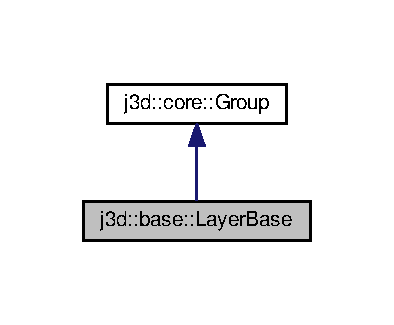
\includegraphics[width=189pt]{classj3d_1_1base_1_1LayerBase__coll__graph}
\end{center}
\end{figure}
\subsection*{Public Member Functions}
\begin{DoxyCompactItemize}
\item 
\hypertarget{classj3d_1_1base_1_1LayerBase_adad4d571ceaaa47d462eb028cd6f5466}{}{\bfseries Layer\+Base} (bool control\+\_\+delete=true)\label{classj3d_1_1base_1_1LayerBase_adad4d571ceaaa47d462eb028cd6f5466}

\item 
\hypertarget{classj3d_1_1base_1_1LayerBase_a7dbc963db84ba07205aeb4789dbaa6c7}{}virtual void {\bfseries pre\+Render} ()\label{classj3d_1_1base_1_1LayerBase_a7dbc963db84ba07205aeb4789dbaa6c7}

\item 
\hypertarget{classj3d_1_1base_1_1LayerBase_a27ec2f264362dd5f6f93c78f3ae5c43c}{}virtual void {\bfseries render} ()\label{classj3d_1_1base_1_1LayerBase_a27ec2f264362dd5f6f93c78f3ae5c43c}

\item 
\hypertarget{classj3d_1_1base_1_1LayerBase_ab947f8f6006b70e95a3c7b1f91f72f35}{}virtual void {\bfseries post\+Render} ()\label{classj3d_1_1base_1_1LayerBase_ab947f8f6006b70e95a3c7b1f91f72f35}

\item 
\hypertarget{classj3d_1_1base_1_1LayerBase_aea32226a5ced8fc6b3bf9148f25ec034}{}\hyperlink{classj3d_1_1base_1_1LayerBase}{Layer\+Base} $\ast$ {\bfseries render\+Buffer} (\hyperlink{classj3d_1_1base_1_1RenderbufferBase}{Renderbuffer\+Base} $\ast$)\label{classj3d_1_1base_1_1LayerBase_aea32226a5ced8fc6b3bf9148f25ec034}

\item 
\hypertarget{classj3d_1_1base_1_1LayerBase_a5999d2361f01fb74b07bea1ec78a6592}{}const \hyperlink{classj3d_1_1base_1_1RenderbufferBase}{Renderbuffer\+Base} $\ast$ {\bfseries render\+Buffer} () const \label{classj3d_1_1base_1_1LayerBase_a5999d2361f01fb74b07bea1ec78a6592}

\end{DoxyCompactItemize}
\subsection*{Additional Inherited Members}


The documentation for this class was generated from the following files\+:\begin{DoxyCompactItemize}
\item 
/media/will/ratchet/\+Projects/\+J\+A\+W/j3d-\/demo/j3d/base/layer\+\_\+base.\+h\item 
/media/will/ratchet/\+Projects/\+J\+A\+W/j3d-\/demo/j3d/base/layer\+\_\+base.\+cpp\end{DoxyCompactItemize}

\hypertarget{classj3d_1_1Light}{}\section{j3d\+:\+:Light Class Reference}
\label{classj3d_1_1Light}\index{j3d\+::\+Light@{j3d\+::\+Light}}


Inheritance diagram for j3d\+:\+:Light\+:
\nopagebreak
\begin{figure}[H]
\begin{center}
\leavevmode
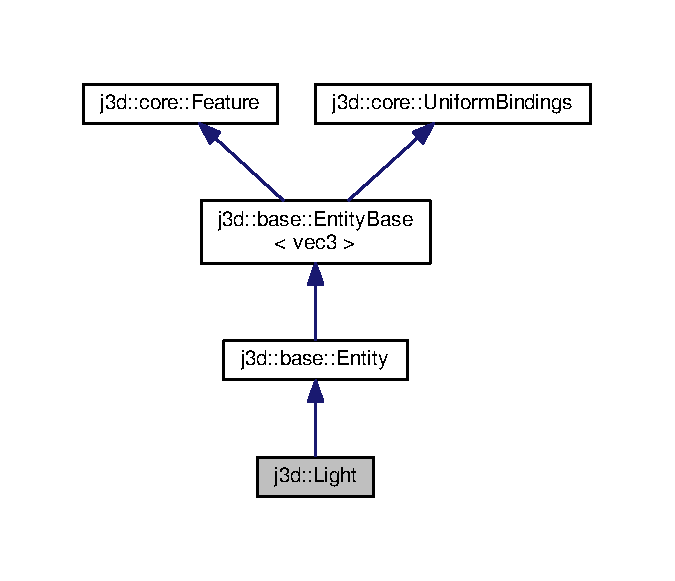
\includegraphics[width=324pt]{classj3d_1_1Light__inherit__graph}
\end{center}
\end{figure}


Collaboration diagram for j3d\+:\+:Light\+:
\nopagebreak
\begin{figure}[H]
\begin{center}
\leavevmode
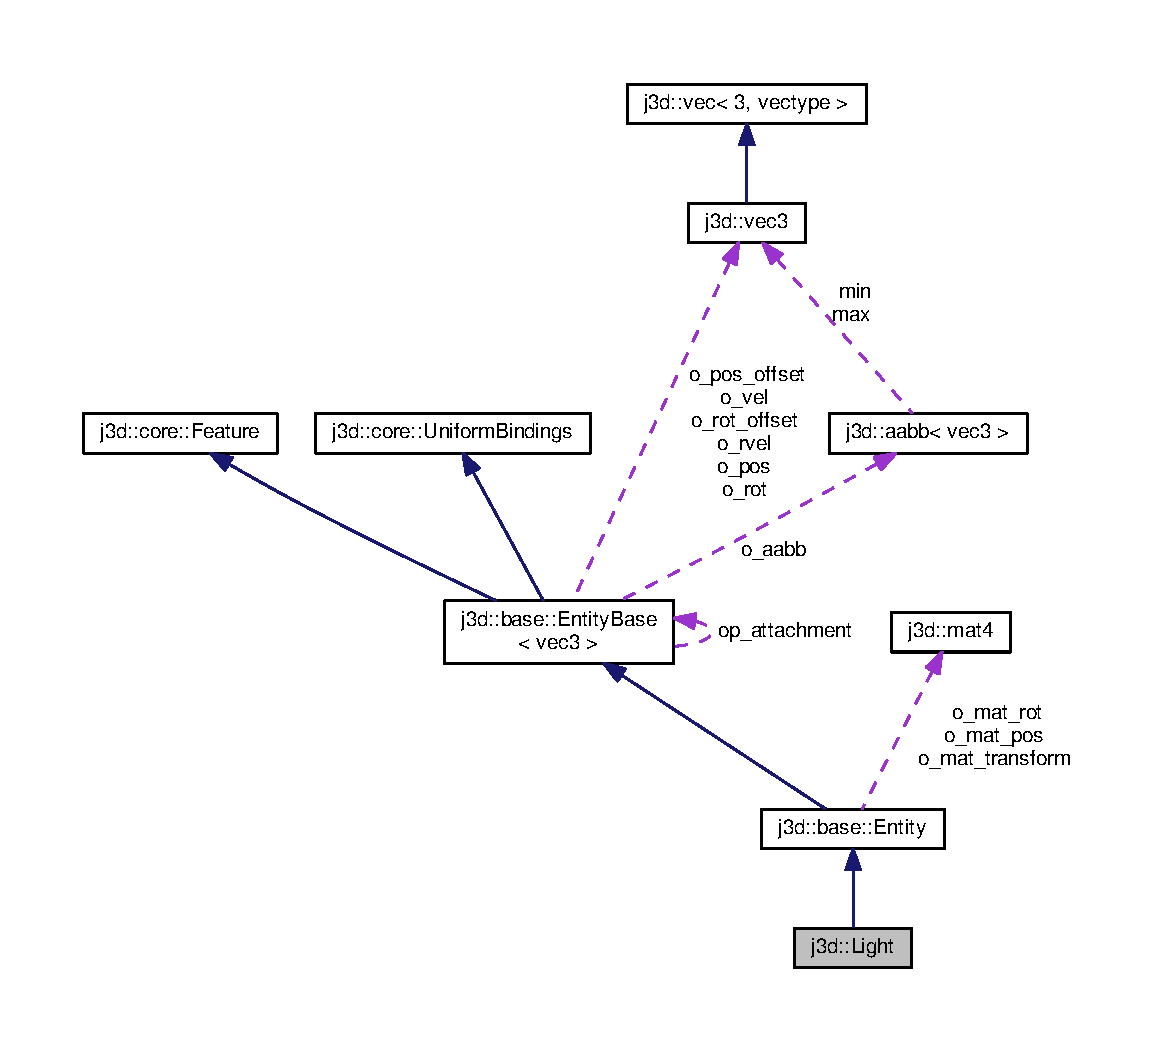
\includegraphics[width=350pt]{classj3d_1_1Light__coll__graph}
\end{center}
\end{figure}
\subsection*{Public Member Functions}
\begin{DoxyCompactItemize}
\item 
\hypertarget{classj3d_1_1Light_af5b37963a0d57a3e176dcf5b849e8a09}{}{\bfseries Light} (light\+\_\+t)\label{classj3d_1_1Light_af5b37963a0d57a3e176dcf5b849e8a09}

\item 
\hypertarget{classj3d_1_1Light_af0d1cafccae6025092e2535d80cd61de}{}{\bfseries Light} (const \hyperlink{structj3d_1_1vec3}{vec3} \&dif, const \hyperlink{structj3d_1_1vec3}{vec3} \&amb, const \hyperlink{structj3d_1_1vec3}{vec3} \&dir, light\+\_\+t=light\+\_\+t\+::\+D\+I\+R\+E\+C\+T\+I\+O\+N\+A\+L)\label{classj3d_1_1Light_af0d1cafccae6025092e2535d80cd61de}

\item 
\hypertarget{classj3d_1_1Light_a8205a8601d85e7ab03f8ae683d5b4631}{}{\bfseries Light} (const \hyperlink{structj3d_1_1vec3}{vec3} \&dif, light\+\_\+t=light\+\_\+t\+::\+P\+O\+I\+N\+T)\label{classj3d_1_1Light_a8205a8601d85e7ab03f8ae683d5b4631}

\item 
\hypertarget{classj3d_1_1Light_a10659d6178d1661871d2f6bf16c0db58}{}{\bfseries Light} (const \hyperlink{structj3d_1_1vec3}{vec3} \&dif, const \hyperlink{structj3d_1_1vec3}{vec3} \&amb, const \hyperlink{structj3d_1_1vec3}{vec3} \&dir, const float \&cos, light\+\_\+t=light\+\_\+t\+::\+S\+P\+O\+T)\label{classj3d_1_1Light_a10659d6178d1661871d2f6bf16c0db58}

\item 
\hypertarget{classj3d_1_1Light_ad1251abf7fb9c2fa0d15ef4150014601}{}void {\bfseries render} ()\label{classj3d_1_1Light_ad1251abf7fb9c2fa0d15ef4150014601}

\item 
\hypertarget{classj3d_1_1Light_a7e8cbad232eab5175285e37ea0e8003b}{}\hyperlink{structj3d_1_1LightProps}{Light\+Props} {\bfseries props} ()\label{classj3d_1_1Light_a7e8cbad232eab5175285e37ea0e8003b}

\item 
\hypertarget{classj3d_1_1Light_a578264f68d470aac1a1f5c574a001422}{}\hyperlink{classj3d_1_1Light}{Light} $\ast$ {\bfseries assign\+Diffuse\+Uniform} (const string \&)\label{classj3d_1_1Light_a578264f68d470aac1a1f5c574a001422}

\item 
\hypertarget{classj3d_1_1Light_a511fd4cce64253d3e6abea96507a07d1}{}\hyperlink{classj3d_1_1Light}{Light} $\ast$ {\bfseries assign\+Ambient\+Uniform} (const string \&)\label{classj3d_1_1Light_a511fd4cce64253d3e6abea96507a07d1}

\item 
\hypertarget{classj3d_1_1Light_aa08b480a557e7749164fa039dda60a73}{}\hyperlink{classj3d_1_1Light}{Light} $\ast$ {\bfseries assign\+Dir\+Uniform} (const string \&)\label{classj3d_1_1Light_aa08b480a557e7749164fa039dda60a73}

\item 
\hypertarget{classj3d_1_1Light_a11620bc320a144501ca617fe66f8b8c6}{}\hyperlink{classj3d_1_1Light}{Light} $\ast$ {\bfseries assign\+Cos\+Uniform} (const string \&)\label{classj3d_1_1Light_a11620bc320a144501ca617fe66f8b8c6}

\item 
\hypertarget{classj3d_1_1Light_a496e633ffeb5e3beba8bc5c39fb15a2c}{}\hyperlink{classj3d_1_1Light}{Light} $\ast$ {\bfseries diffuse} (const \hyperlink{structj3d_1_1vec3}{vec3} \&)\label{classj3d_1_1Light_a496e633ffeb5e3beba8bc5c39fb15a2c}

\item 
\hypertarget{classj3d_1_1Light_a2248a7ed6df70c9140a4354d672503a8}{}\hyperlink{classj3d_1_1Light}{Light} $\ast$ {\bfseries ambient} (const \hyperlink{structj3d_1_1vec3}{vec3} \&)\label{classj3d_1_1Light_a2248a7ed6df70c9140a4354d672503a8}

\item 
\hypertarget{classj3d_1_1Light_a5fca118f0a9c893c11f9db10b8ef74e3}{}\hyperlink{classj3d_1_1Light}{Light} $\ast$ {\bfseries dir} (const \hyperlink{structj3d_1_1vec3}{vec3} \&)\label{classj3d_1_1Light_a5fca118f0a9c893c11f9db10b8ef74e3}

\item 
\hypertarget{classj3d_1_1Light_af49a744ae93aab354f934aaf12ce6c9f}{}\hyperlink{classj3d_1_1Light}{Light} $\ast$ {\bfseries cos} (const float \&)\label{classj3d_1_1Light_af49a744ae93aab354f934aaf12ce6c9f}

\item 
\hypertarget{classj3d_1_1Light_a8be1975b798d3206c5a5ffa2a9bc71df}{}const \hyperlink{structj3d_1_1vec3}{vec3} \& {\bfseries diffuse} () const \label{classj3d_1_1Light_a8be1975b798d3206c5a5ffa2a9bc71df}

\item 
\hypertarget{classj3d_1_1Light_a6da703f0a03b9f6fed86d81f6b6c7ba8}{}const \hyperlink{structj3d_1_1vec3}{vec3} \& {\bfseries ambient} () const \label{classj3d_1_1Light_a6da703f0a03b9f6fed86d81f6b6c7ba8}

\item 
\hypertarget{classj3d_1_1Light_ac41ce7275ae4b8b2de86c83c313cf548}{}const \hyperlink{structj3d_1_1vec3}{vec3} \& {\bfseries dir} () const \label{classj3d_1_1Light_ac41ce7275ae4b8b2de86c83c313cf548}

\item 
\hypertarget{classj3d_1_1Light_a2d2507340b759685f5f84e34cba6ac3b}{}const float \& {\bfseries cos} () const \label{classj3d_1_1Light_a2d2507340b759685f5f84e34cba6ac3b}

\end{DoxyCompactItemize}
\subsection*{Additional Inherited Members}


The documentation for this class was generated from the following files\+:\begin{DoxyCompactItemize}
\item 
/media/will/ratchet/\+Projects/\+J\+A\+W/j3d-\/demo/j3d/light.\+h\item 
/media/will/ratchet/\+Projects/\+J\+A\+W/j3d-\/demo/j3d/light.\+cpp\end{DoxyCompactItemize}

\hypertarget{structj3d_1_1LightProps}{}\section{j3d\+:\+:Light\+Props Struct Reference}
\label{structj3d_1_1LightProps}\index{j3d\+::\+Light\+Props@{j3d\+::\+Light\+Props}}


Collaboration diagram for j3d\+:\+:Light\+Props\+:
\nopagebreak
\begin{figure}[H]
\begin{center}
\leavevmode
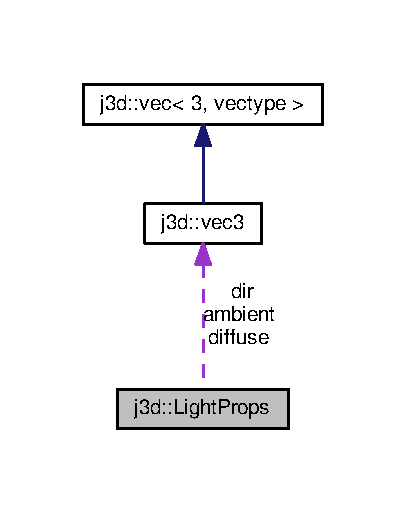
\includegraphics[width=195pt]{structj3d_1_1LightProps__coll__graph}
\end{center}
\end{figure}
\subsection*{Data Fields}
\begin{DoxyCompactItemize}
\item 
\hypertarget{structj3d_1_1LightProps_a063a0292ff76b4d23dc89a45ea11c0fd}{}\hyperlink{structj3d_1_1vec3}{vec3} \& {\bfseries diffuse}\label{structj3d_1_1LightProps_a063a0292ff76b4d23dc89a45ea11c0fd}

\item 
\hypertarget{structj3d_1_1LightProps_a6543c47398038d83da7dbcb72d496d54}{}\hyperlink{structj3d_1_1vec3}{vec3} \& {\bfseries ambient}\label{structj3d_1_1LightProps_a6543c47398038d83da7dbcb72d496d54}

\item 
\hypertarget{structj3d_1_1LightProps_a23994a43d3779c7ea0aa567b1c2ad8b9}{}\hyperlink{structj3d_1_1vec3}{vec3} \& {\bfseries dir}\label{structj3d_1_1LightProps_a23994a43d3779c7ea0aa567b1c2ad8b9}

\item 
\hypertarget{structj3d_1_1LightProps_ab345d2308a17b174326cb1e0f62890aa}{}float \& {\bfseries cos}\label{structj3d_1_1LightProps_ab345d2308a17b174326cb1e0f62890aa}

\end{DoxyCompactItemize}


The documentation for this struct was generated from the following file\+:\begin{DoxyCompactItemize}
\item 
/media/will/ratchet/\+Projects/\+J\+A\+W/j3d-\/demo/j3d/light.\+h\end{DoxyCompactItemize}

\hypertarget{structj3d_1_1mat4}{}\section{j3d\+:\+:mat4 Struct Reference}
\label{structj3d_1_1mat4}\index{j3d\+::mat4@{j3d\+::mat4}}
\subsection*{Public Member Functions}
\begin{DoxyCompactItemize}
\item 
\hypertarget{structj3d_1_1mat4_a56f35bdc345aaa44b6aeebb0cf1ab5b5}{}float {\bfseries get} (const int \&r, const int \&c)\label{structj3d_1_1mat4_a56f35bdc345aaa44b6aeebb0cf1ab5b5}

\item 
\hypertarget{structj3d_1_1mat4_a4acf4de8b23af2dc83c51903687416aa}{}void {\bfseries set} (const int \&r, const int \&c, const float \&val)\label{structj3d_1_1mat4_a4acf4de8b23af2dc83c51903687416aa}

\item 
\hypertarget{structj3d_1_1mat4_a40cd857e569497a08b23b361a7243d0d}{}float \& {\bfseries at} (const int \&i)\label{structj3d_1_1mat4_a40cd857e569497a08b23b361a7243d0d}

\item 
\hypertarget{structj3d_1_1mat4_a7aa70b303ee99806515439eb1b7cf448}{}void {\bfseries zero} ()\label{structj3d_1_1mat4_a7aa70b303ee99806515439eb1b7cf448}

\item 
\hypertarget{structj3d_1_1mat4_a71898d110967c8765eab35dda0478db9}{}void {\bfseries iden} ()\label{structj3d_1_1mat4_a71898d110967c8765eab35dda0478db9}

\item 
\hypertarget{structj3d_1_1mat4_a9f0cc218b95a55a9d0e54cc47286595e}{}\hyperlink{structj3d_1_1mat4}{mat4} \& {\bfseries invert} ()\label{structj3d_1_1mat4_a9f0cc218b95a55a9d0e54cc47286595e}

\item 
\hypertarget{structj3d_1_1mat4_a8acfa6d69b75310a4aac587829f1abd7}{}\hyperlink{structj3d_1_1mat4}{mat4} {\bfseries inverse} ()\label{structj3d_1_1mat4_a8acfa6d69b75310a4aac587829f1abd7}

\item 
\hypertarget{structj3d_1_1mat4_ad093d6001bddef5b63f1521d051f89e6}{}void {\bfseries inverse} (\hyperlink{structj3d_1_1mat4}{mat4} $\ast$m)\label{structj3d_1_1mat4_ad093d6001bddef5b63f1521d051f89e6}

\item 
\hypertarget{structj3d_1_1mat4_a9a71377f2c96a29f471befda124d60d7}{}\hyperlink{structj3d_1_1mat4}{mat4} \& {\bfseries operator=} (const \hyperlink{structj3d_1_1mat4}{mat4} \&m)\label{structj3d_1_1mat4_a9a71377f2c96a29f471befda124d60d7}

\item 
\hypertarget{structj3d_1_1mat4_ab14982474a28b0ebf2601388e0155c6a}{}\hyperlink{structj3d_1_1mat4}{mat4} \& {\bfseries operator$\ast$=} (const \hyperlink{structj3d_1_1mat4}{mat4} \&m)\label{structj3d_1_1mat4_ab14982474a28b0ebf2601388e0155c6a}

\item 
\hypertarget{structj3d_1_1mat4_a25bc83b10d8f478916cca0bb9c61bd60}{}float \& {\bfseries operator\mbox{[}$\,$\mbox{]}} (const int \&i)\label{structj3d_1_1mat4_a25bc83b10d8f478916cca0bb9c61bd60}

\item 
\hypertarget{structj3d_1_1mat4_a151d90e204efdcffa8940b8b0d541233}{}\hyperlink{structj3d_1_1mat4}{mat4} {\bfseries operator$\ast$} (const \hyperlink{structj3d_1_1mat4}{mat4} m)\label{structj3d_1_1mat4_a151d90e204efdcffa8940b8b0d541233}

\item 
\hypertarget{structj3d_1_1mat4_a60fd63eefecd4d85278cb744481fe27c}{}{\bfseries operator G\+Lfloat $\ast$} ()\label{structj3d_1_1mat4_a60fd63eefecd4d85278cb744481fe27c}

\end{DoxyCompactItemize}
\subsection*{Data Fields}
\begin{DoxyCompactItemize}
\item 
\hypertarget{structj3d_1_1mat4_a13193f5aeaa5a2daaf50563b3c62439d}{}float {\bfseries data} \mbox{[}4\mbox{]}\mbox{[}4\mbox{]}\label{structj3d_1_1mat4_a13193f5aeaa5a2daaf50563b3c62439d}

\end{DoxyCompactItemize}
\subsection*{Friends}
\begin{DoxyCompactItemize}
\item 
\hypertarget{structj3d_1_1mat4_aa8eb074e83309a02a5ef896ca5eb65c6}{}ostream \& {\bfseries operator$<$$<$} (ostream \&, const \hyperlink{structj3d_1_1mat4}{mat4} \&)\label{structj3d_1_1mat4_aa8eb074e83309a02a5ef896ca5eb65c6}

\end{DoxyCompactItemize}


The documentation for this struct was generated from the following file\+:\begin{DoxyCompactItemize}
\item 
/media/will/ratchet/\+Projects/\+J\+A\+W/j3d-\/demo/j3d/math/matrix.\+h\end{DoxyCompactItemize}

\hypertarget{structj3d_1_1math}{}\section{j3d\+:\+:math Struct Reference}
\label{structj3d_1_1math}\index{j3d\+::math@{j3d\+::math}}
\subsection*{Static Public Member Functions}
\begin{DoxyCompactItemize}
\item 
\hypertarget{structj3d_1_1math_a355d66b7249e52cdadff841434d255bc}{}static float {\bfseries min} (float a, float b)\label{structj3d_1_1math_a355d66b7249e52cdadff841434d255bc}

\item 
\hypertarget{structj3d_1_1math_a7787bfe471d28520d2221ea460ba0dd8}{}static float {\bfseries max} (float a, float b)\label{structj3d_1_1math_a7787bfe471d28520d2221ea460ba0dd8}

\end{DoxyCompactItemize}


The documentation for this struct was generated from the following file\+:\begin{DoxyCompactItemize}
\item 
/media/will/ratchet/\+Projects/\+J\+A\+W/j3d-\/demo/j3d/math/math.\+h\end{DoxyCompactItemize}

\hypertarget{structj3d_1_1matrix}{}\section{j3d\+:\+:matrix Struct Reference}
\label{structj3d_1_1matrix}\index{j3d\+::matrix@{j3d\+::matrix}}
\subsection*{Static Public Member Functions}
\begin{DoxyCompactItemize}
\item 
\hypertarget{structj3d_1_1matrix_ac24b3a1ccdf5685b76e35e3983155553}{}static void {\bfseries translation} (\hyperlink{structj3d_1_1mat4}{mat4} $\ast$m, const \hyperlink{structj3d_1_1vec}{vec}$<$ 3, float $>$ \&v)\label{structj3d_1_1matrix_ac24b3a1ccdf5685b76e35e3983155553}

\item 
\hypertarget{structj3d_1_1matrix_a3bcefb1f8e597ed864c10ddc362e053d}{}static void {\bfseries rotation\+\_\+x} (\hyperlink{structj3d_1_1mat4}{mat4} $\ast$m, const float \&f)\label{structj3d_1_1matrix_a3bcefb1f8e597ed864c10ddc362e053d}

\item 
\hypertarget{structj3d_1_1matrix_a697383b57468099867f18be52229e9a5}{}static void {\bfseries rotation\+\_\+y} (\hyperlink{structj3d_1_1mat4}{mat4} $\ast$m, const float \&f)\label{structj3d_1_1matrix_a697383b57468099867f18be52229e9a5}

\item 
\hypertarget{structj3d_1_1matrix_a1865b6ce825c48f4b095eab6d4b6f669}{}static void {\bfseries rotation\+\_\+z} (\hyperlink{structj3d_1_1mat4}{mat4} $\ast$m, const float \&f)\label{structj3d_1_1matrix_a1865b6ce825c48f4b095eab6d4b6f669}

\item 
\hypertarget{structj3d_1_1matrix_a3ca34a730865f7072bfb8c763452c9cb}{}static void {\bfseries rotation} (\hyperlink{structj3d_1_1mat4}{mat4} $\ast$m, const \hyperlink{structj3d_1_1vec}{vec}$<$ 3, float $>$ \&v)\label{structj3d_1_1matrix_a3ca34a730865f7072bfb8c763452c9cb}

\item 
\hypertarget{structj3d_1_1matrix_a6474eafe5b54e5d9781a578098ced664}{}static void {\bfseries perspective} (\hyperlink{structj3d_1_1mat4}{mat4} $\ast$m, float l, float r, float b, float t, float n, float f)\label{structj3d_1_1matrix_a6474eafe5b54e5d9781a578098ced664}

\end{DoxyCompactItemize}


The documentation for this struct was generated from the following files\+:\begin{DoxyCompactItemize}
\item 
/media/will/ratchet/\+Projects/\+J\+A\+W/j3d-\/demo/j3d/math/matrix.\+h\item 
/media/will/ratchet/\+Projects/\+J\+A\+W/j3d-\/demo/j3d/math/matrix.\+cpp\end{DoxyCompactItemize}

\hypertarget{classj3d_1_1Mesh}{}\section{j3d\+:\+:Mesh Class Reference}
\label{classj3d_1_1Mesh}\index{j3d\+::\+Mesh@{j3d\+::\+Mesh}}


Inheritance diagram for j3d\+:\+:Mesh\+:
\nopagebreak
\begin{figure}[H]
\begin{center}
\leavevmode
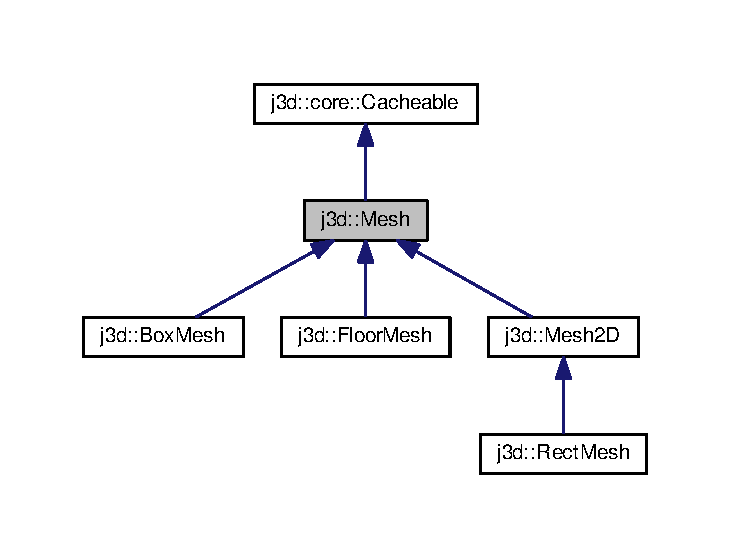
\includegraphics[width=350pt]{classj3d_1_1Mesh__inherit__graph}
\end{center}
\end{figure}


Collaboration diagram for j3d\+:\+:Mesh\+:
\nopagebreak
\begin{figure}[H]
\begin{center}
\leavevmode
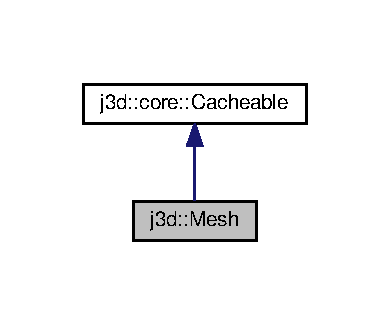
\includegraphics[width=187pt]{classj3d_1_1Mesh__coll__graph}
\end{center}
\end{figure}
\subsection*{Public Member Functions}
\begin{DoxyCompactItemize}
\item 
\hypertarget{classj3d_1_1Mesh_a50845e2441dd6a47535a46681b75a61b}{}{\bfseries Mesh} (const char $\ast$id, mesh\+\_\+draw\+\_\+t=mesh\+\_\+draw\+\_\+t\+::\+A\+R\+R\+A\+Y, mesh\+\_\+shape\+\_\+t=mesh\+\_\+shape\+\_\+t\+::\+T\+R\+I\+A\+N\+G\+L\+E\+S, unsigned int restart\+\_\+index=0)\label{classj3d_1_1Mesh_a50845e2441dd6a47535a46681b75a61b}

\item 
\hypertarget{classj3d_1_1Mesh_a0424c1252d3e0102509a1e711c10871a}{}\hyperlink{classj3d_1_1Mesh}{Mesh} $\ast$ {\bfseries push\+Vertex} (const \hyperlink{structj3d_1_1vec4}{vec4} \&)\label{classj3d_1_1Mesh_a0424c1252d3e0102509a1e711c10871a}

\item 
\hypertarget{classj3d_1_1Mesh_ad2706e1df7e487c98e92ced73b0a4868}{}\hyperlink{classj3d_1_1Mesh}{Mesh} $\ast$ {\bfseries push\+Vertices} (const \hyperlink{structj3d_1_1vec4}{vec4} $\ast$, const unsigned int \&len)\label{classj3d_1_1Mesh_ad2706e1df7e487c98e92ced73b0a4868}

\item 
\hypertarget{classj3d_1_1Mesh_aba0d1a333fbbe08088f5eeb7d215d4fe}{}\hyperlink{classj3d_1_1Mesh}{Mesh} $\ast$ {\bfseries push\+Vertices} (initializer\+\_\+list$<$ \hyperlink{structj3d_1_1vec4}{vec4} $>$)\label{classj3d_1_1Mesh_aba0d1a333fbbe08088f5eeb7d215d4fe}

\item 
\hypertarget{classj3d_1_1Mesh_a16c0372e4b7ef6c04e5b264d2713c764}{}\hyperlink{classj3d_1_1Mesh}{Mesh} $\ast$ {\bfseries push\+Vertex} (const \hyperlink{structj3d_1_1vec3}{vec3} \&)\label{classj3d_1_1Mesh_a16c0372e4b7ef6c04e5b264d2713c764}

\item 
\hypertarget{classj3d_1_1Mesh_ad7e82524f542ece78233996704b29249}{}\hyperlink{classj3d_1_1Mesh}{Mesh} $\ast$ {\bfseries push\+Vertices} (const \hyperlink{structj3d_1_1vec3}{vec3} $\ast$, const unsigned int \&len)\label{classj3d_1_1Mesh_ad7e82524f542ece78233996704b29249}

\item 
\hypertarget{classj3d_1_1Mesh_a653940f151ce28564b72eb3d835aa721}{}\hyperlink{classj3d_1_1Mesh}{Mesh} $\ast$ {\bfseries push\+Vertices} (initializer\+\_\+list$<$ \hyperlink{structj3d_1_1vec3}{vec3} $>$)\label{classj3d_1_1Mesh_a653940f151ce28564b72eb3d835aa721}

\item 
\hypertarget{classj3d_1_1Mesh_add174405f0afe0442c65867d5e23f417}{}\hyperlink{classj3d_1_1Mesh}{Mesh} $\ast$ {\bfseries push\+Vertex} (const \hyperlink{structj3d_1_1vec2}{vec2} \&)\label{classj3d_1_1Mesh_add174405f0afe0442c65867d5e23f417}

\item 
\hypertarget{classj3d_1_1Mesh_a0a2c34d440ea1fa82320798d5f43d9a8}{}\hyperlink{classj3d_1_1Mesh}{Mesh} $\ast$ {\bfseries push\+Vertices} (const \hyperlink{structj3d_1_1vec2}{vec2} $\ast$, const unsigned int \&len)\label{classj3d_1_1Mesh_a0a2c34d440ea1fa82320798d5f43d9a8}

\item 
\hypertarget{classj3d_1_1Mesh_ab3202bad7bf7e180eacbb0c3410607bf}{}\hyperlink{classj3d_1_1Mesh}{Mesh} $\ast$ {\bfseries push\+Vertices} (initializer\+\_\+list$<$ \hyperlink{structj3d_1_1vec2}{vec2} $>$)\label{classj3d_1_1Mesh_ab3202bad7bf7e180eacbb0c3410607bf}

\item 
\hypertarget{classj3d_1_1Mesh_ad60a48983a6787008d2b380a1db2a729}{}\hyperlink{classj3d_1_1Mesh}{Mesh} $\ast$ {\bfseries push\+Normal} (const \hyperlink{structj3d_1_1vec3}{vec3} \&)\label{classj3d_1_1Mesh_ad60a48983a6787008d2b380a1db2a729}

\item 
\hypertarget{classj3d_1_1Mesh_a98003392f9f323c7416cf1654a660956}{}\hyperlink{classj3d_1_1Mesh}{Mesh} $\ast$ {\bfseries push\+Normals} (const \hyperlink{structj3d_1_1vec3}{vec3} $\ast$, const unsigned int \&len)\label{classj3d_1_1Mesh_a98003392f9f323c7416cf1654a660956}

\item 
\hypertarget{classj3d_1_1Mesh_a9369a90e560398ff05fd30cb6c1897c8}{}\hyperlink{classj3d_1_1Mesh}{Mesh} $\ast$ {\bfseries push\+Normals} (initializer\+\_\+list$<$ \hyperlink{structj3d_1_1vec3}{vec3} $>$)\label{classj3d_1_1Mesh_a9369a90e560398ff05fd30cb6c1897c8}

\item 
\hypertarget{classj3d_1_1Mesh_a38376550db6060e51b88ed54b327d44e}{}\hyperlink{classj3d_1_1Mesh}{Mesh} $\ast$ {\bfseries push\+Index} (const unsigned int \&)\label{classj3d_1_1Mesh_a38376550db6060e51b88ed54b327d44e}

\item 
\hypertarget{classj3d_1_1Mesh_a111eca316406e214f9f3a11836879453}{}\hyperlink{classj3d_1_1Mesh}{Mesh} $\ast$ {\bfseries push\+Indices} (const unsigned int $\ast$, const unsigned int \&len)\label{classj3d_1_1Mesh_a111eca316406e214f9f3a11836879453}

\item 
\hypertarget{classj3d_1_1Mesh_a2effb08bcef93493ef5f1dd585ae2f95}{}\hyperlink{classj3d_1_1Mesh}{Mesh} $\ast$ {\bfseries push\+Indices} (initializer\+\_\+list$<$ unsigned int $>$)\label{classj3d_1_1Mesh_a2effb08bcef93493ef5f1dd585ae2f95}

\item 
\hypertarget{classj3d_1_1Mesh_a20bb2c2c6e241e5cf278af3fd8b3059b}{}virtual void {\bfseries build} ()\label{classj3d_1_1Mesh_a20bb2c2c6e241e5cf278af3fd8b3059b}

\item 
\hypertarget{classj3d_1_1Mesh_a5237bc1186c7ecaa1af79738e3d7db50}{}virtual void {\bfseries bind} ()\label{classj3d_1_1Mesh_a5237bc1186c7ecaa1af79738e3d7db50}

\item 
\hypertarget{classj3d_1_1Mesh_aa196429f3e87ecd53e8770ba979222f4}{}virtual void {\bfseries render} ()\label{classj3d_1_1Mesh_aa196429f3e87ecd53e8770ba979222f4}

\item 
\hypertarget{classj3d_1_1Mesh_a1becd0d472967c2d7797bdb17a8e2bed}{}\hyperlink{classj3d_1_1Mesh}{Mesh} $\ast$ {\bfseries optimize2\+D} (bool=true)\label{classj3d_1_1Mesh_a1becd0d472967c2d7797bdb17a8e2bed}

\item 
\hypertarget{classj3d_1_1Mesh_a95c05b5ad0db2262fa1bee52e486045b}{}bool {\bfseries optimize2\+D} () const \label{classj3d_1_1Mesh_a95c05b5ad0db2262fa1bee52e486045b}

\item 
\hypertarget{classj3d_1_1Mesh_a295a8de2d8af946c4cbca8f8636faa2b}{}const \hyperlink{structj3d_1_1vec3}{vec3} \& {\bfseries min} () const \label{classj3d_1_1Mesh_a295a8de2d8af946c4cbca8f8636faa2b}

\item 
\hypertarget{classj3d_1_1Mesh_ac4e88a913a5865dc2019cd4a5d25bcd0}{}const \hyperlink{structj3d_1_1vec3}{vec3} \& {\bfseries max} () const \label{classj3d_1_1Mesh_ac4e88a913a5865dc2019cd4a5d25bcd0}

\end{DoxyCompactItemize}
\subsection*{Static Public Attributes}
\begin{DoxyCompactItemize}
\item 
\hypertarget{classj3d_1_1Mesh_a5ae57c2edc8bb9609fd720d6fe8eb7de}{}static const char constexpr $\ast$ {\bfseries J3\+D\+\_\+\+C\+A\+C\+H\+E\+\_\+\+I\+D} = \char`\"{}mesh\char`\"{}\label{classj3d_1_1Mesh_a5ae57c2edc8bb9609fd720d6fe8eb7de}

\end{DoxyCompactItemize}


The documentation for this class was generated from the following files\+:\begin{DoxyCompactItemize}
\item 
/media/will/ratchet/\+Projects/\+J\+A\+W/j3d-\/demo/j3d/mesh.\+h\item 
/media/will/ratchet/\+Projects/\+J\+A\+W/j3d-\/demo/j3d/mesh.\+cpp\end{DoxyCompactItemize}

\hypertarget{classj3d_1_1Mesh2D}{}\section{j3d\+:\+:Mesh2\+D Class Reference}
\label{classj3d_1_1Mesh2D}\index{j3d\+::\+Mesh2\+D@{j3d\+::\+Mesh2\+D}}


Inheritance diagram for j3d\+:\+:Mesh2\+D\+:
\nopagebreak
\begin{figure}[H]
\begin{center}
\leavevmode
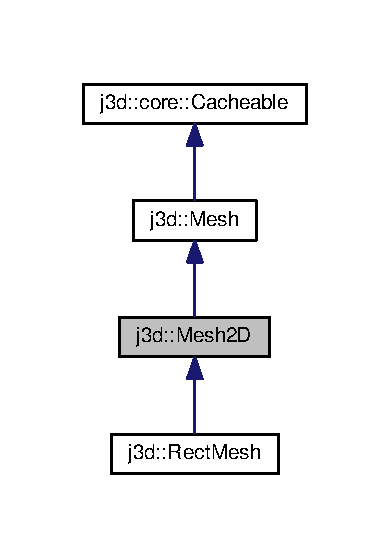
\includegraphics[width=187pt]{classj3d_1_1Mesh2D__inherit__graph}
\end{center}
\end{figure}


Collaboration diagram for j3d\+:\+:Mesh2\+D\+:
\nopagebreak
\begin{figure}[H]
\begin{center}
\leavevmode
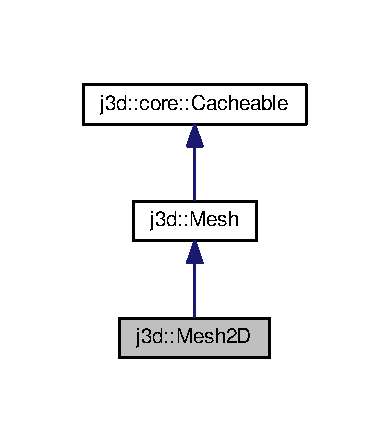
\includegraphics[width=187pt]{classj3d_1_1Mesh2D__coll__graph}
\end{center}
\end{figure}
\subsection*{Public Member Functions}
\begin{DoxyCompactItemize}
\item 
\hypertarget{classj3d_1_1Mesh2D_a02973553a23ee4ad8e6c391032df7b44}{}{\bfseries Mesh2\+D} (const char $\ast$id, mesh\+\_\+draw\+\_\+t=mesh\+\_\+draw\+\_\+t\+::\+A\+R\+R\+A\+Y, mesh\+\_\+shape\+\_\+t=mesh\+\_\+shape\+\_\+t\+::\+T\+R\+I\+A\+N\+G\+L\+E\+S, unsigned int restart\+\_\+index=0)\label{classj3d_1_1Mesh2D_a02973553a23ee4ad8e6c391032df7b44}

\end{DoxyCompactItemize}
\subsection*{Additional Inherited Members}


The documentation for this class was generated from the following files\+:\begin{DoxyCompactItemize}
\item 
/media/will/ratchet/\+Projects/\+J\+A\+W/j3d-\/demo/j3d/mesh\+\_\+2d.\+h\item 
/media/will/ratchet/\+Projects/\+J\+A\+W/j3d-\/demo/j3d/mesh\+\_\+2d.\+cpp\end{DoxyCompactItemize}

\hypertarget{classMeshTest}{}\section{Mesh\+Test Class Reference}
\label{classMeshTest}\index{Mesh\+Test@{Mesh\+Test}}


Inheritance diagram for Mesh\+Test\+:
\nopagebreak
\begin{figure}[H]
\begin{center}
\leavevmode
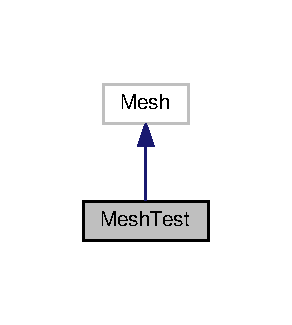
\includegraphics[width=140pt]{classMeshTest__inherit__graph}
\end{center}
\end{figure}


Collaboration diagram for Mesh\+Test\+:
\nopagebreak
\begin{figure}[H]
\begin{center}
\leavevmode
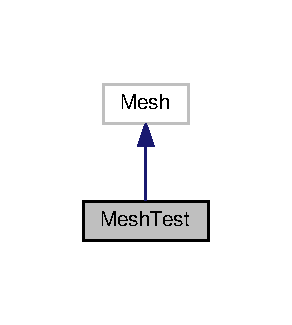
\includegraphics[width=140pt]{classMeshTest__coll__graph}
\end{center}
\end{figure}
\subsection*{Public Member Functions}
\begin{DoxyCompactItemize}
\item 
\hypertarget{classMeshTest_aca09ed80b9c3ee0daf802a0b631903e2}{}{\bfseries Mesh\+Test} (const char $\ast$id)\label{classMeshTest_aca09ed80b9c3ee0daf802a0b631903e2}

\end{DoxyCompactItemize}


The documentation for this class was generated from the following files\+:\begin{DoxyCompactItemize}
\item 
/media/will/ratchet/\+Projects/\+J\+A\+W/j3d-\/demo/demo/mesh\+\_\+test.\+h\item 
/media/will/ratchet/\+Projects/\+J\+A\+W/j3d-\/demo/demo/mesh\+\_\+test.\+cpp\end{DoxyCompactItemize}

\hypertarget{classj3d_1_1Object}{}\section{j3d\+:\+:Object Class Reference}
\label{classj3d_1_1Object}\index{j3d\+::\+Object@{j3d\+::\+Object}}


Inheritance diagram for j3d\+:\+:Object\+:
\nopagebreak
\begin{figure}[H]
\begin{center}
\leavevmode
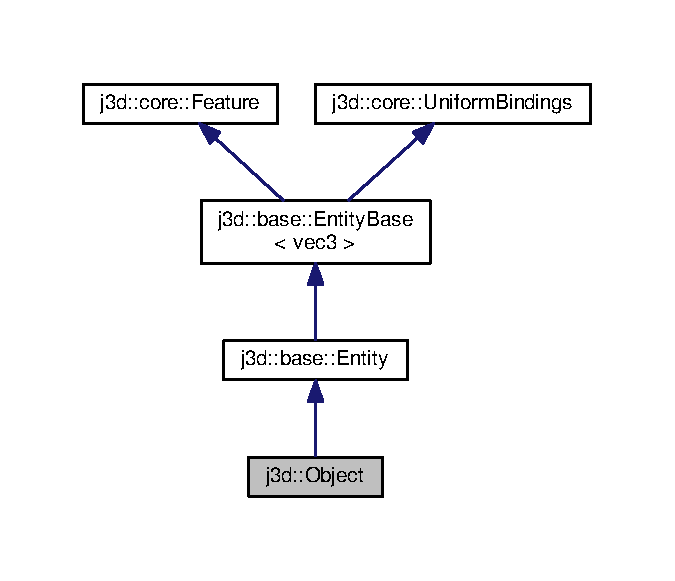
\includegraphics[width=324pt]{classj3d_1_1Object__inherit__graph}
\end{center}
\end{figure}


Collaboration diagram for j3d\+:\+:Object\+:
\nopagebreak
\begin{figure}[H]
\begin{center}
\leavevmode
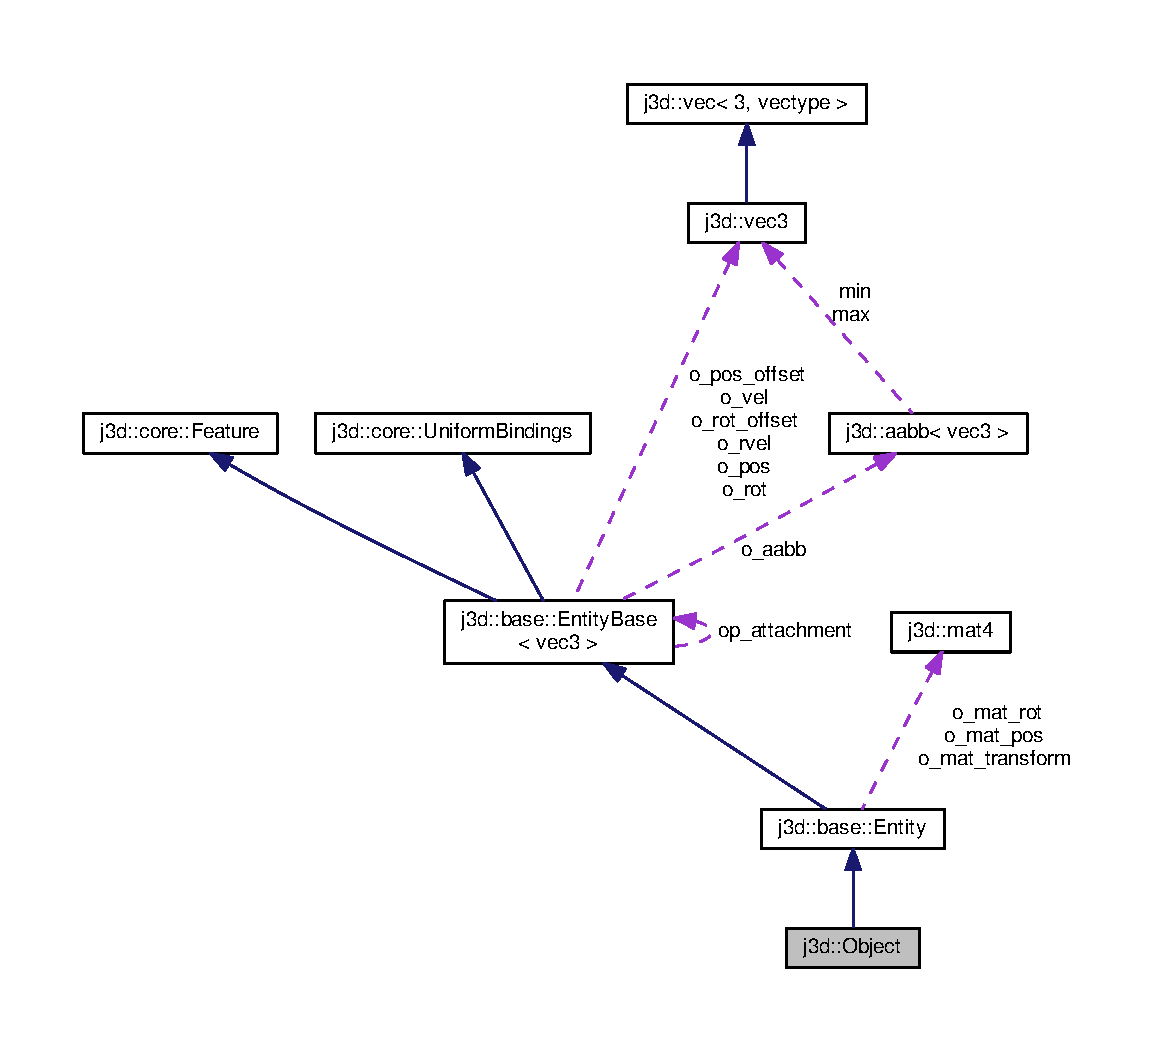
\includegraphics[width=350pt]{classj3d_1_1Object__coll__graph}
\end{center}
\end{figure}
\subsection*{Public Member Functions}
\begin{DoxyCompactItemize}
\item 
\hypertarget{classj3d_1_1Object_a7dcade6be931c20e74a3e1ff1cb52b4f}{}{\bfseries Object} (const string \&mesh\+\_\+id)\label{classj3d_1_1Object_a7dcade6be931c20e74a3e1ff1cb52b4f}

\item 
\hypertarget{classj3d_1_1Object_a6d2910f06b85e547eac3b6b4842af9dc}{}{\bfseries Object} (const string \&mesh\+\_\+id, const string \&shader\+\_\+id)\label{classj3d_1_1Object_a6d2910f06b85e547eac3b6b4842af9dc}

\item 
\hypertarget{classj3d_1_1Object_a4abd48bacb1b004c8ac891597c831f77}{}virtual void {\bfseries update} ()\label{classj3d_1_1Object_a4abd48bacb1b004c8ac891597c831f77}

\item 
\hypertarget{classj3d_1_1Object_ae0e92359520b9a848f45efdd86485552}{}virtual void {\bfseries render} ()\label{classj3d_1_1Object_ae0e92359520b9a848f45efdd86485552}

\end{DoxyCompactItemize}
\subsection*{Additional Inherited Members}


The documentation for this class was generated from the following files\+:\begin{DoxyCompactItemize}
\item 
/media/will/ratchet/\+Projects/\+J\+A\+W/j3d-\/demo/j3d/object.\+h\item 
/media/will/ratchet/\+Projects/\+J\+A\+W/j3d-\/demo/j3d/object.\+cpp\end{DoxyCompactItemize}

\hypertarget{structj3d_1_1ray}{}\section{j3d\+:\+:ray$<$ T $>$ Struct Template Reference}
\label{structj3d_1_1ray}\index{j3d\+::ray$<$ T $>$@{j3d\+::ray$<$ T $>$}}


Collaboration diagram for j3d\+:\+:ray$<$ T $>$\+:
\nopagebreak
\begin{figure}[H]
\begin{center}
\leavevmode
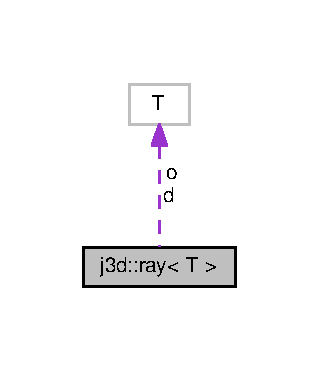
\includegraphics[width=153pt]{structj3d_1_1ray__coll__graph}
\end{center}
\end{figure}
\subsection*{Public Member Functions}
\begin{DoxyCompactItemize}
\item 
\hypertarget{structj3d_1_1ray_a555276083aafd278de35d4a0620acdf7}{}{\bfseries ray} (const \hyperlink{structj3d_1_1ray}{ray} \&r)\label{structj3d_1_1ray_a555276083aafd278de35d4a0620acdf7}

\item 
\hypertarget{structj3d_1_1ray_aac9d526d9bc60813f4af179d8c515c6b}{}{\bfseries ray} (const T \&\+\_\+o, const T \&\+\_\+d)\label{structj3d_1_1ray_aac9d526d9bc60813f4af179d8c515c6b}

\item 
\hypertarget{structj3d_1_1ray_a31c660ce6b0f90fa12ecc7d0ec55b31f}{}\hyperlink{structj3d_1_1ray}{ray} \& {\bfseries assign} (const \hyperlink{structj3d_1_1ray}{ray}$<$ T $>$ \&r)\label{structj3d_1_1ray_a31c660ce6b0f90fa12ecc7d0ec55b31f}

\item 
\hypertarget{structj3d_1_1ray_a18c4a5d94aa38283e1a636a71014c66c}{}\hyperlink{structj3d_1_1ray}{ray} \& {\bfseries assign} (const T \&\+\_\+o, const T \&\+\_\+d)\label{structj3d_1_1ray_a18c4a5d94aa38283e1a636a71014c66c}

\end{DoxyCompactItemize}
\subsection*{Data Fields}
\begin{DoxyCompactItemize}
\item 
\hypertarget{structj3d_1_1ray_a37e81619c53928fb39a795c3c2cb7429}{}T {\bfseries o}\label{structj3d_1_1ray_a37e81619c53928fb39a795c3c2cb7429}

\item 
\hypertarget{structj3d_1_1ray_ad61a092f6d24ee93754a9d0737f54c2f}{}T {\bfseries d}\label{structj3d_1_1ray_ad61a092f6d24ee93754a9d0737f54c2f}

\end{DoxyCompactItemize}
\subsection*{Friends}
\begin{DoxyCompactItemize}
\item 
\hypertarget{structj3d_1_1ray_ab3d1ca1bda6bf1df96a457983abf2e50}{}{\footnotesize template$<$class $>$ }\\ostream \& {\bfseries operator$<$$<$} (ostream \&, const \hyperlink{structj3d_1_1ray}{ray}$<$ T $>$ \&)\label{structj3d_1_1ray_ab3d1ca1bda6bf1df96a457983abf2e50}

\end{DoxyCompactItemize}


The documentation for this struct was generated from the following file\+:\begin{DoxyCompactItemize}
\item 
/media/will/ratchet/\+Projects/\+J\+A\+W/j3d-\/demo/j3d/math/ray.\+h\end{DoxyCompactItemize}

\hypertarget{structj3d_1_1ray3}{}\section{j3d\+:\+:ray3 Struct Reference}
\label{structj3d_1_1ray3}\index{j3d\+::ray3@{j3d\+::ray3}}


Inheritance diagram for j3d\+:\+:ray3\+:
\nopagebreak
\begin{figure}[H]
\begin{center}
\leavevmode
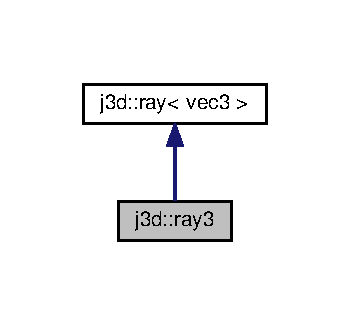
\includegraphics[width=168pt]{structj3d_1_1ray3__inherit__graph}
\end{center}
\end{figure}


Collaboration diagram for j3d\+:\+:ray3\+:
\nopagebreak
\begin{figure}[H]
\begin{center}
\leavevmode
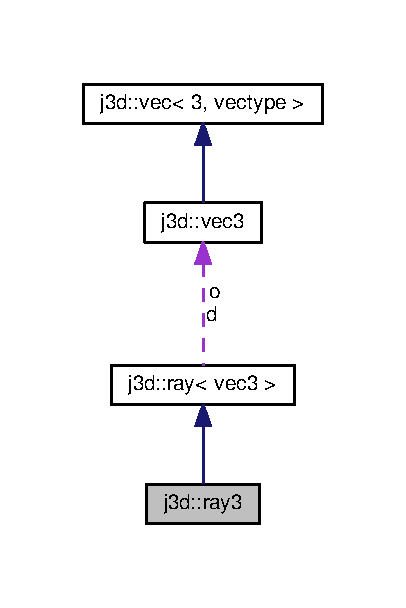
\includegraphics[width=195pt]{structj3d_1_1ray3__coll__graph}
\end{center}
\end{figure}
\subsection*{Public Member Functions}
\begin{DoxyCompactItemize}
\item 
\hypertarget{structj3d_1_1ray3_aa5238e8fac4d6bc809e300c37da66806}{}\hyperlink{structj3d_1_1ray3}{ray3} \& {\bfseries from\+\_\+window} (int win\+\_\+x, int win\+\_\+y)\label{structj3d_1_1ray3_aa5238e8fac4d6bc809e300c37da66806}

\end{DoxyCompactItemize}
\subsection*{Additional Inherited Members}


The documentation for this struct was generated from the following files\+:\begin{DoxyCompactItemize}
\item 
/media/will/ratchet/\+Projects/\+J\+A\+W/j3d-\/demo/j3d/math/ray.\+h\item 
/media/will/ratchet/\+Projects/\+J\+A\+W/j3d-\/demo/j3d/math/ray.\+cpp\end{DoxyCompactItemize}

\hypertarget{classj3d_1_1RectMesh}{}\section{j3d\+:\+:Rect\+Mesh Class Reference}
\label{classj3d_1_1RectMesh}\index{j3d\+::\+Rect\+Mesh@{j3d\+::\+Rect\+Mesh}}


Inheritance diagram for j3d\+:\+:Rect\+Mesh\+:
\nopagebreak
\begin{figure}[H]
\begin{center}
\leavevmode
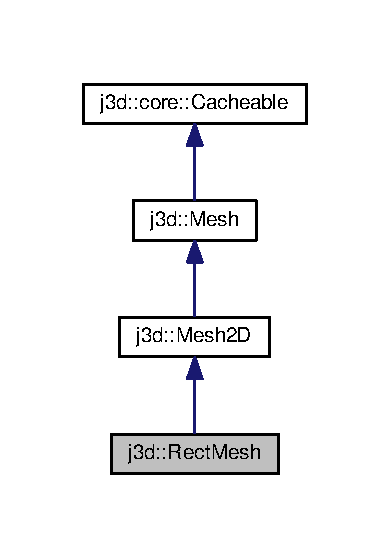
\includegraphics[width=187pt]{classj3d_1_1RectMesh__inherit__graph}
\end{center}
\end{figure}


Collaboration diagram for j3d\+:\+:Rect\+Mesh\+:
\nopagebreak
\begin{figure}[H]
\begin{center}
\leavevmode
\includegraphics[width=187pt]{classj3d_1_1RectMesh__coll__graph}
\end{center}
\end{figure}
\subsection*{Public Member Functions}
\begin{DoxyCompactItemize}
\item 
\hypertarget{classj3d_1_1RectMesh_a63087a6a6614881925619442287b47b4}{}{\bfseries Rect\+Mesh} (const char $\ast$id, float t, float r, float b, float l)\label{classj3d_1_1RectMesh_a63087a6a6614881925619442287b47b4}

\item 
\hypertarget{classj3d_1_1RectMesh_a956d8994c6cade28e972caac7a9122e8}{}float {\bfseries top} () const \label{classj3d_1_1RectMesh_a956d8994c6cade28e972caac7a9122e8}

\item 
\hypertarget{classj3d_1_1RectMesh_a1acd5ba6f2dc67d212c3556cd0a02a16}{}float {\bfseries right} () const \label{classj3d_1_1RectMesh_a1acd5ba6f2dc67d212c3556cd0a02a16}

\item 
\hypertarget{classj3d_1_1RectMesh_af385d9f24e73e0508c1119d91e1e83e3}{}float {\bfseries left} () const \label{classj3d_1_1RectMesh_af385d9f24e73e0508c1119d91e1e83e3}

\item 
\hypertarget{classj3d_1_1RectMesh_a34eb4d65e52126bd4a1816c36d6b107c}{}float {\bfseries bottom} () const \label{classj3d_1_1RectMesh_a34eb4d65e52126bd4a1816c36d6b107c}

\end{DoxyCompactItemize}
\subsection*{Additional Inherited Members}


The documentation for this class was generated from the following files\+:\begin{DoxyCompactItemize}
\item 
/media/will/ratchet/\+Projects/\+J\+A\+W/j3d-\/demo/j3d/mesh\+\_\+shapes.\+h\item 
/media/will/ratchet/\+Projects/\+J\+A\+W/j3d-\/demo/j3d/mesh\+\_\+shapes.\+cpp\end{DoxyCompactItemize}

\hypertarget{classj3d_1_1base_1_1Renderbuffer}{}\section{j3d\+:\+:base\+:\+:Renderbuffer Class Reference}
\label{classj3d_1_1base_1_1Renderbuffer}\index{j3d\+::base\+::\+Renderbuffer@{j3d\+::base\+::\+Renderbuffer}}


Inheritance diagram for j3d\+:\+:base\+:\+:Renderbuffer\+:
\nopagebreak
\begin{figure}[H]
\begin{center}
\leavevmode
\includegraphics[width=221pt]{classj3d_1_1base_1_1Renderbuffer__inherit__graph}
\end{center}
\end{figure}


Collaboration diagram for j3d\+:\+:base\+:\+:Renderbuffer\+:
\nopagebreak
\begin{figure}[H]
\begin{center}
\leavevmode
\includegraphics[width=221pt]{classj3d_1_1base_1_1Renderbuffer__coll__graph}
\end{center}
\end{figure}
\subsection*{Public Member Functions}
\begin{DoxyCompactItemize}
\item 
\hypertarget{classj3d_1_1base_1_1Renderbuffer_a0cac34555f49c7c11f0c6fdc6d561e6c}{}void {\bfseries reshape} (int x, int y)\label{classj3d_1_1base_1_1Renderbuffer_a0cac34555f49c7c11f0c6fdc6d561e6c}

\item 
\hypertarget{classj3d_1_1base_1_1Renderbuffer_a337ccff301db4504b3a44a60ade88fe5}{}void {\bfseries bind} ()\label{classj3d_1_1base_1_1Renderbuffer_a337ccff301db4504b3a44a60ade88fe5}

\item 
\hypertarget{classj3d_1_1base_1_1Renderbuffer_a20fe4f3f3d794323d0feceeb9f49f178}{}void {\bfseries blit} ()\label{classj3d_1_1base_1_1Renderbuffer_a20fe4f3f3d794323d0feceeb9f49f178}

\end{DoxyCompactItemize}
\subsection*{Static Public Attributes}
\begin{DoxyCompactItemize}
\item 
\hypertarget{classj3d_1_1base_1_1Renderbuffer_a89ddb3deee083d573fb02d7da3c1baa4}{}static const int {\bfseries N\+U\+M\+\_\+\+B\+U\+F\+F\+E\+R\+S} = 2\label{classj3d_1_1base_1_1Renderbuffer_a89ddb3deee083d573fb02d7da3c1baa4}

\item 
\hypertarget{classj3d_1_1base_1_1Renderbuffer_abfeb2086204c39280423a71f770a5992}{}static const int {\bfseries C\+O\+L\+O\+R\+\_\+\+B\+U\+F\+F\+E\+R} = 0\label{classj3d_1_1base_1_1Renderbuffer_abfeb2086204c39280423a71f770a5992}

\item 
\hypertarget{classj3d_1_1base_1_1Renderbuffer_a54526410287ad7f79aed589f9c9f7dcb}{}static const int {\bfseries D\+E\+P\+T\+H\+\_\+\+B\+U\+F\+F\+E\+R} = 1\label{classj3d_1_1base_1_1Renderbuffer_a54526410287ad7f79aed589f9c9f7dcb}

\end{DoxyCompactItemize}


The documentation for this class was generated from the following files\+:\begin{DoxyCompactItemize}
\item 
/media/will/ratchet/\+Projects/\+J\+A\+W/j3d-\/demo/j3d/base/renderbuffer.\+h\item 
/media/will/ratchet/\+Projects/\+J\+A\+W/j3d-\/demo/j3d/base/renderbuffer.\+cpp\end{DoxyCompactItemize}

\hypertarget{classj3d_1_1base_1_1Renderbuffer2D}{}\section{j3d\+:\+:base\+:\+:Renderbuffer2\+D Class Reference}
\label{classj3d_1_1base_1_1Renderbuffer2D}\index{j3d\+::base\+::\+Renderbuffer2\+D@{j3d\+::base\+::\+Renderbuffer2\+D}}


Inheritance diagram for j3d\+:\+:base\+:\+:Renderbuffer2\+D\+:
\nopagebreak
\begin{figure}[H]
\begin{center}
\leavevmode
\includegraphics[width=221pt]{classj3d_1_1base_1_1Renderbuffer2D__inherit__graph}
\end{center}
\end{figure}


Collaboration diagram for j3d\+:\+:base\+:\+:Renderbuffer2\+D\+:
\nopagebreak
\begin{figure}[H]
\begin{center}
\leavevmode
\includegraphics[width=221pt]{classj3d_1_1base_1_1Renderbuffer2D__coll__graph}
\end{center}
\end{figure}
\subsection*{Public Member Functions}
\begin{DoxyCompactItemize}
\item 
\hypertarget{classj3d_1_1base_1_1Renderbuffer2D_a00f70f33dd8433635a765f5c10e2c234}{}void {\bfseries reshape} (int x, int y)\label{classj3d_1_1base_1_1Renderbuffer2D_a00f70f33dd8433635a765f5c10e2c234}

\item 
\hypertarget{classj3d_1_1base_1_1Renderbuffer2D_a24cf4da6d9f6e69d0f514732d78e8fb4}{}void {\bfseries bind} ()\label{classj3d_1_1base_1_1Renderbuffer2D_a24cf4da6d9f6e69d0f514732d78e8fb4}

\item 
\hypertarget{classj3d_1_1base_1_1Renderbuffer2D_af8e98b3af5b027fa51dd9a31d5219cea}{}void {\bfseries blit} ()\label{classj3d_1_1base_1_1Renderbuffer2D_af8e98b3af5b027fa51dd9a31d5219cea}

\end{DoxyCompactItemize}
\subsection*{Additional Inherited Members}


The documentation for this class was generated from the following files\+:\begin{DoxyCompactItemize}
\item 
/media/will/ratchet/\+Projects/\+J\+A\+W/j3d-\/demo/j3d/base/renderbuffer\+\_\+2d.\+h\item 
/media/will/ratchet/\+Projects/\+J\+A\+W/j3d-\/demo/j3d/base/renderbuffer\+\_\+2d.\+cpp\end{DoxyCompactItemize}

\hypertarget{classj3d_1_1base_1_1RenderbufferBase}{}\section{j3d\+:\+:base\+:\+:Renderbuffer\+Base Class Reference}
\label{classj3d_1_1base_1_1RenderbufferBase}\index{j3d\+::base\+::\+Renderbuffer\+Base@{j3d\+::base\+::\+Renderbuffer\+Base}}


Inheritance diagram for j3d\+:\+:base\+:\+:Renderbuffer\+Base\+:
\nopagebreak
\begin{figure}[H]
\begin{center}
\leavevmode
\includegraphics[width=348pt]{classj3d_1_1base_1_1RenderbufferBase__inherit__graph}
\end{center}
\end{figure}


Collaboration diagram for j3d\+:\+:base\+:\+:Renderbuffer\+Base\+:
\nopagebreak
\begin{figure}[H]
\begin{center}
\leavevmode
\includegraphics[width=221pt]{classj3d_1_1base_1_1RenderbufferBase__coll__graph}
\end{center}
\end{figure}
\subsection*{Public Member Functions}
\begin{DoxyCompactItemize}
\item 
\hypertarget{classj3d_1_1base_1_1RenderbufferBase_a4d46858cdbeb14059b966103f49b1e6d}{}virtual void {\bfseries reshape} (int x, int y)\label{classj3d_1_1base_1_1RenderbufferBase_a4d46858cdbeb14059b966103f49b1e6d}

\item 
\hypertarget{classj3d_1_1base_1_1RenderbufferBase_acdfb90724dbd6d440037c739cb591544}{}virtual void {\bfseries bind} ()=0\label{classj3d_1_1base_1_1RenderbufferBase_acdfb90724dbd6d440037c739cb591544}

\item 
\hypertarget{classj3d_1_1base_1_1RenderbufferBase_aef0d7158533b26949cac74017bbbead7}{}virtual void {\bfseries blit} ()=0\label{classj3d_1_1base_1_1RenderbufferBase_aef0d7158533b26949cac74017bbbead7}

\end{DoxyCompactItemize}
\subsection*{Additional Inherited Members}


The documentation for this class was generated from the following file\+:\begin{DoxyCompactItemize}
\item 
/media/will/ratchet/\+Projects/\+J\+A\+W/j3d-\/demo/j3d/base/renderbuffer\+\_\+base.\+h\end{DoxyCompactItemize}

\hypertarget{classj3d_1_1core_1_1ReshapeBatch}{}\section{j3d\+:\+:core\+:\+:Reshape\+Batch Class Reference}
\label{classj3d_1_1core_1_1ReshapeBatch}\index{j3d\+::core\+::\+Reshape\+Batch@{j3d\+::core\+::\+Reshape\+Batch}}


Inheritance diagram for j3d\+:\+:core\+:\+:Reshape\+Batch\+:
\nopagebreak
\begin{figure}[H]
\begin{center}
\leavevmode
\includegraphics[width=350pt]{classj3d_1_1core_1_1ReshapeBatch__inherit__graph}
\end{center}
\end{figure}


Collaboration diagram for j3d\+:\+:core\+:\+:Reshape\+Batch\+:
\nopagebreak
\begin{figure}[H]
\begin{center}
\leavevmode
\includegraphics[width=205pt]{classj3d_1_1core_1_1ReshapeBatch__coll__graph}
\end{center}
\end{figure}
\subsection*{Public Member Functions}
\begin{DoxyCompactItemize}
\item 
\hypertarget{classj3d_1_1core_1_1ReshapeBatch_ac3bcf95cb9a212c831309666c7fe8474}{}virtual void {\bfseries reshape} (int w, int h)\label{classj3d_1_1core_1_1ReshapeBatch_ac3bcf95cb9a212c831309666c7fe8474}

\end{DoxyCompactItemize}
\subsection*{Static Public Attributes}
\begin{DoxyCompactItemize}
\item 
\hypertarget{classj3d_1_1core_1_1ReshapeBatch_a025eb21b8151c9ae11e4a77c3717e117}{}static const char constexpr $\ast$ {\bfseries J3\+D\+\_\+\+B\+A\+T\+C\+H\+\_\+\+I\+D} = \char`\"{}j3d\+\_\+reshape\char`\"{}\label{classj3d_1_1core_1_1ReshapeBatch_a025eb21b8151c9ae11e4a77c3717e117}

\end{DoxyCompactItemize}


The documentation for this class was generated from the following file\+:\begin{DoxyCompactItemize}
\item 
/media/will/ratchet/\+Projects/\+J\+A\+W/j3d-\/demo/j3d/core/reshape\+\_\+batch.\+h\end{DoxyCompactItemize}

\hypertarget{classj3d_1_1Scene}{}\section{j3d\+:\+:Scene Class Reference}
\label{classj3d_1_1Scene}\index{j3d\+::\+Scene@{j3d\+::\+Scene}}


Inheritance diagram for j3d\+:\+:Scene\+:
\nopagebreak
\begin{figure}[H]
\begin{center}
\leavevmode
\includegraphics[width=322pt]{classj3d_1_1Scene__inherit__graph}
\end{center}
\end{figure}


Collaboration diagram for j3d\+:\+:Scene\+:
\nopagebreak
\begin{figure}[H]
\begin{center}
\leavevmode
\includegraphics[width=322pt]{classj3d_1_1Scene__coll__graph}
\end{center}
\end{figure}
\subsection*{Public Member Functions}
\begin{DoxyCompactItemize}
\item 
\hypertarget{classj3d_1_1Scene_a3943ddb5181afafce79d85cd3ebbd752}{}{\bfseries Scene} (const char $\ast$id, bool activate=true)\label{classj3d_1_1Scene_a3943ddb5181afafce79d85cd3ebbd752}

\item 
\hypertarget{classj3d_1_1Scene_a300c15b700a256b1ad0e55323b1491f0}{}void {\bfseries cache\+Activate} ()\label{classj3d_1_1Scene_a300c15b700a256b1ad0e55323b1491f0}

\item 
\hypertarget{classj3d_1_1Scene_adf671a288f878e3efa42ccbf34b0d6ed}{}void {\bfseries activate} ()\label{classj3d_1_1Scene_adf671a288f878e3efa42ccbf34b0d6ed}

\end{DoxyCompactItemize}
\subsection*{Static Public Attributes}
\begin{DoxyCompactItemize}
\item 
\hypertarget{classj3d_1_1Scene_ae37dfe706793bf75401ae547de727914}{}static const char constexpr $\ast$ {\bfseries J3\+D\+\_\+\+C\+A\+C\+H\+E\+\_\+\+I\+D} = \char`\"{}scene\char`\"{}\label{classj3d_1_1Scene_ae37dfe706793bf75401ae547de727914}

\end{DoxyCompactItemize}
\subsection*{Protected Member Functions}
\begin{DoxyCompactItemize}
\item 
\hypertarget{classj3d_1_1Scene_a8ef39136a6566bba72a8aef5fd99be1c}{}virtual void {\bfseries load} ()\label{classj3d_1_1Scene_a8ef39136a6566bba72a8aef5fd99be1c}

\item 
\hypertarget{classj3d_1_1Scene_a2fbbca36c8b7063cd6d1e0743da438a9}{}virtual void {\bfseries unload} ()\label{classj3d_1_1Scene_a2fbbca36c8b7063cd6d1e0743da438a9}

\item 
\hypertarget{classj3d_1_1Scene_a79d797457dfb3ef93313bad9b5e5c6fc}{}virtual void {\bfseries update} ()\label{classj3d_1_1Scene_a79d797457dfb3ef93313bad9b5e5c6fc}

\end{DoxyCompactItemize}
\subsection*{Friends}
\begin{DoxyCompactItemize}
\item 
\hypertarget{classj3d_1_1Scene_a614ec0a1871249dee57baf50d4501271}{}class {\bfseries engine}\label{classj3d_1_1Scene_a614ec0a1871249dee57baf50d4501271}

\end{DoxyCompactItemize}


The documentation for this class was generated from the following files\+:\begin{DoxyCompactItemize}
\item 
/media/will/ratchet/\+Projects/\+J\+A\+W/j3d-\/demo/j3d/scene.\+h\item 
/media/will/ratchet/\+Projects/\+J\+A\+W/j3d-\/demo/j3d/scene.\+cpp\end{DoxyCompactItemize}

\hypertarget{classj3d_1_1ShaderProgram_1_1Shader}{}\section{j3d\+:\+:Shader\+Program\+:\+:Shader Class Reference}
\label{classj3d_1_1ShaderProgram_1_1Shader}\index{j3d\+::\+Shader\+Program\+::\+Shader@{j3d\+::\+Shader\+Program\+::\+Shader}}


Inheritance diagram for j3d\+:\+:Shader\+Program\+:\+:Shader\+:
\nopagebreak
\begin{figure}[H]
\begin{center}
\leavevmode
\includegraphics[width=304pt]{classj3d_1_1ShaderProgram_1_1Shader__inherit__graph}
\end{center}
\end{figure}


Collaboration diagram for j3d\+:\+:Shader\+Program\+:\+:Shader\+:
\nopagebreak
\begin{figure}[H]
\begin{center}
\leavevmode
\includegraphics[width=187pt]{classj3d_1_1ShaderProgram_1_1Shader__coll__graph}
\end{center}
\end{figure}
\subsection*{Public Member Functions}
\begin{DoxyCompactItemize}
\item 
\hypertarget{classj3d_1_1ShaderProgram_1_1Shader_abc71dc01c2917b32dfb3040dcb5f9e0b}{}{\bfseries Shader} (const char $\ast$path, G\+Lenum type)\label{classj3d_1_1ShaderProgram_1_1Shader_abc71dc01c2917b32dfb3040dcb5f9e0b}

\item 
\hypertarget{classj3d_1_1ShaderProgram_1_1Shader_af793368e86747dda96c3c372a4a80bbc}{}G\+Lenum {\bfseries type} () const \label{classj3d_1_1ShaderProgram_1_1Shader_af793368e86747dda96c3c372a4a80bbc}

\item 
\hypertarget{classj3d_1_1ShaderProgram_1_1Shader_ac5fdb3bfe00d0fef2b88783f98c59843}{}G\+Luint {\bfseries id} () const \label{classj3d_1_1ShaderProgram_1_1Shader_ac5fdb3bfe00d0fef2b88783f98c59843}

\end{DoxyCompactItemize}
\subsection*{Static Public Attributes}
\begin{DoxyCompactItemize}
\item 
\hypertarget{classj3d_1_1ShaderProgram_1_1Shader_a20f3b954a556f5fc2c30cf12e0a29a9c}{}static const char constexpr $\ast$ {\bfseries J3\+D\+\_\+\+C\+A\+C\+H\+E\+\_\+\+I\+D} = \char`\"{}shader\char`\"{}\label{classj3d_1_1ShaderProgram_1_1Shader_a20f3b954a556f5fc2c30cf12e0a29a9c}

\end{DoxyCompactItemize}
\subsection*{Protected Attributes}
\begin{DoxyCompactItemize}
\item 
\hypertarget{classj3d_1_1ShaderProgram_1_1Shader_a3f84fddc2b154de37b8e9632bc10c7f8}{}G\+Lenum {\bfseries o\+\_\+type}\label{classj3d_1_1ShaderProgram_1_1Shader_a3f84fddc2b154de37b8e9632bc10c7f8}

\item 
\hypertarget{classj3d_1_1ShaderProgram_1_1Shader_accf4054b26f49c1ac24f96c54330c028}{}G\+Luint {\bfseries o\+\_\+id}\label{classj3d_1_1ShaderProgram_1_1Shader_accf4054b26f49c1ac24f96c54330c028}

\end{DoxyCompactItemize}


The documentation for this class was generated from the following files\+:\begin{DoxyCompactItemize}
\item 
/media/will/ratchet/\+Projects/\+J\+A\+W/j3d-\/demo/j3d/shader.\+h\item 
/media/will/ratchet/\+Projects/\+J\+A\+W/j3d-\/demo/j3d/shader.\+cpp\end{DoxyCompactItemize}

\hypertarget{classj3d_1_1ShaderProgram}{}\section{j3d\+:\+:Shader\+Program Class Reference}
\label{classj3d_1_1ShaderProgram}\index{j3d\+::\+Shader\+Program@{j3d\+::\+Shader\+Program}}


Inheritance diagram for j3d\+:\+:Shader\+Program\+:
\nopagebreak
\begin{figure}[H]
\begin{center}
\leavevmode
\includegraphics[width=338pt]{classj3d_1_1ShaderProgram__inherit__graph}
\end{center}
\end{figure}


Collaboration diagram for j3d\+:\+:Shader\+Program\+:
\nopagebreak
\begin{figure}[H]
\begin{center}
\leavevmode
\includegraphics[width=338pt]{classj3d_1_1ShaderProgram__coll__graph}
\end{center}
\end{figure}
\subsection*{Data Structures}
\begin{DoxyCompactItemize}
\item 
class \hyperlink{classj3d_1_1ShaderProgram_1_1FragmentShader}{Fragment\+Shader}
\item 
class \hyperlink{classj3d_1_1ShaderProgram_1_1Shader}{Shader}
\item 
class \hyperlink{classj3d_1_1ShaderProgram_1_1VertexShader}{Vertex\+Shader}
\end{DoxyCompactItemize}
\subsection*{Public Member Functions}
\begin{DoxyCompactItemize}
\item 
\hypertarget{classj3d_1_1ShaderProgram_a256861bced49d6b74052b369565e0a3a}{}{\bfseries Shader\+Program} (const char $\ast$id)\label{classj3d_1_1ShaderProgram_a256861bced49d6b74052b369565e0a3a}

\item 
\hypertarget{classj3d_1_1ShaderProgram_aabf534b9674a8c6e6bc3fc282b58370a}{}\hyperlink{classj3d_1_1ShaderProgram}{Shader\+Program} $\ast$ {\bfseries add\+Vertex\+Shader} (const char $\ast$path)\label{classj3d_1_1ShaderProgram_aabf534b9674a8c6e6bc3fc282b58370a}

\item 
\hypertarget{classj3d_1_1ShaderProgram_a55413493fe237ef5d44b37a49dcd007f}{}\hyperlink{classj3d_1_1ShaderProgram}{Shader\+Program} $\ast$ {\bfseries add\+Fragment\+Shader} (const char $\ast$path)\label{classj3d_1_1ShaderProgram_a55413493fe237ef5d44b37a49dcd007f}

\item 
\hypertarget{classj3d_1_1ShaderProgram_a5a254033a2f7262925b60e0341cf2faf}{}void {\bfseries link} (initializer\+\_\+list$<$ const char $\ast$ $>$ unames, bool use=true)\label{classj3d_1_1ShaderProgram_a5a254033a2f7262925b60e0341cf2faf}

\item 
\hypertarget{classj3d_1_1ShaderProgram_a51af6878076ba30d66d31729d2246cc8}{}void {\bfseries use} ()\label{classj3d_1_1ShaderProgram_a51af6878076ba30d66d31729d2246cc8}

\item 
\hypertarget{classj3d_1_1ShaderProgram_a1853b5309e07793de4bd144cf019c382}{}bool {\bfseries has\+Uniform} (const char $\ast$key, bool debug\+\_\+fatal=true)\label{classj3d_1_1ShaderProgram_a1853b5309e07793de4bd144cf019c382}

\item 
\hypertarget{classj3d_1_1ShaderProgram_a3112b9db7e260459fbee7e72660bff11}{}\hyperlink{classj3d_1_1ShaderProgram}{Shader\+Program} $\ast$ {\bfseries bind} (const char $\ast$key, \hyperlink{structj3d_1_1vec2}{vec2} v)\label{classj3d_1_1ShaderProgram_a3112b9db7e260459fbee7e72660bff11}

\item 
\hypertarget{classj3d_1_1ShaderProgram_a3cbc41a16d6a452405b754914cf7562b}{}\hyperlink{classj3d_1_1ShaderProgram}{Shader\+Program} $\ast$ {\bfseries bind} (const char $\ast$key, \hyperlink{structj3d_1_1vec3}{vec3} v)\label{classj3d_1_1ShaderProgram_a3cbc41a16d6a452405b754914cf7562b}

\item 
\hypertarget{classj3d_1_1ShaderProgram_a5eddbfaadf6fd550a1a603b8f8662dfd}{}\hyperlink{classj3d_1_1ShaderProgram}{Shader\+Program} $\ast$ {\bfseries bind} (const char $\ast$key, \hyperlink{structj3d_1_1vec4}{vec4} v)\label{classj3d_1_1ShaderProgram_a5eddbfaadf6fd550a1a603b8f8662dfd}

\item 
\hypertarget{classj3d_1_1ShaderProgram_a16c12cb76e91a9ffd65d5fb15abcfe1c}{}\hyperlink{classj3d_1_1ShaderProgram}{Shader\+Program} $\ast$ {\bfseries bind} (const char $\ast$key, \hyperlink{structj3d_1_1mat4}{mat4} m)\label{classj3d_1_1ShaderProgram_a16c12cb76e91a9ffd65d5fb15abcfe1c}

\item 
\hypertarget{classj3d_1_1ShaderProgram_a29c32f30181b9d32c4ebcd2a1f8ac9d1}{}G\+Luint {\bfseries id} () const \label{classj3d_1_1ShaderProgram_a29c32f30181b9d32c4ebcd2a1f8ac9d1}

\item 
\hypertarget{classj3d_1_1ShaderProgram_a65c6128b795a9a67d49e471ee6f1abcf}{}bool {\bfseries linked} () const \label{classj3d_1_1ShaderProgram_a65c6128b795a9a67d49e471ee6f1abcf}

\item 
\hypertarget{classj3d_1_1ShaderProgram_a255692aee26f1c3f405e841d9999fa29}{}G\+Lint {\bfseries uloc} (const char $\ast$key) const \label{classj3d_1_1ShaderProgram_a255692aee26f1c3f405e841d9999fa29}

\end{DoxyCompactItemize}
\subsection*{Static Public Attributes}
\begin{DoxyCompactItemize}
\item 
\hypertarget{classj3d_1_1ShaderProgram_af54405ccdbe123c9b13c061726553ce1}{}static const char constexpr $\ast$ {\bfseries J3\+D\+\_\+\+C\+A\+C\+H\+E\+\_\+\+I\+D} = \char`\"{}shaderprogram\char`\"{}\label{classj3d_1_1ShaderProgram_af54405ccdbe123c9b13c061726553ce1}

\item 
\hypertarget{classj3d_1_1ShaderProgram_a2d04080fbe4a4acff8ebcdc046334f88}{}static const int {\bfseries S\+H\+A\+D\+E\+R\+\_\+\+C\+O\+U\+N\+T} = 2\label{classj3d_1_1ShaderProgram_a2d04080fbe4a4acff8ebcdc046334f88}

\end{DoxyCompactItemize}


The documentation for this class was generated from the following files\+:\begin{DoxyCompactItemize}
\item 
/media/will/ratchet/\+Projects/\+J\+A\+W/j3d-\/demo/j3d/shader.\+h\item 
/media/will/ratchet/\+Projects/\+J\+A\+W/j3d-\/demo/j3d/shader.\+cpp\end{DoxyCompactItemize}

\hypertarget{classj3d_1_1Sprite}{}\section{j3d\+:\+:Sprite Class Reference}
\label{classj3d_1_1Sprite}\index{j3d\+::\+Sprite@{j3d\+::\+Sprite}}


Inheritance diagram for j3d\+:\+:Sprite\+:
\nopagebreak
\begin{figure}[H]
\begin{center}
\leavevmode
\includegraphics[width=324pt]{classj3d_1_1Sprite__inherit__graph}
\end{center}
\end{figure}


Collaboration diagram for j3d\+:\+:Sprite\+:
\nopagebreak
\begin{figure}[H]
\begin{center}
\leavevmode
\includegraphics[width=350pt]{classj3d_1_1Sprite__coll__graph}
\end{center}
\end{figure}
\subsection*{Public Member Functions}
\begin{DoxyCompactItemize}
\item 
\hypertarget{classj3d_1_1Sprite_a7392601fc95ec39c80157bd96a62ad66}{}{\bfseries Sprite} (const char $\ast$mesh\+\_\+id)\label{classj3d_1_1Sprite_a7392601fc95ec39c80157bd96a62ad66}

\item 
\hypertarget{classj3d_1_1Sprite_a59154f8d2e82ba5de5e119ec5d3c0826}{}virtual void {\bfseries update} ()\label{classj3d_1_1Sprite_a59154f8d2e82ba5de5e119ec5d3c0826}

\item 
\hypertarget{classj3d_1_1Sprite_a05623afcb83eed0a9fce70561f06a2fe}{}virtual void {\bfseries render} ()\label{classj3d_1_1Sprite_a05623afcb83eed0a9fce70561f06a2fe}

\end{DoxyCompactItemize}
\subsection*{Additional Inherited Members}


The documentation for this class was generated from the following files\+:\begin{DoxyCompactItemize}
\item 
/media/will/ratchet/\+Projects/\+J\+A\+W/j3d-\/demo/j3d/sprite.\+h\item 
/media/will/ratchet/\+Projects/\+J\+A\+W/j3d-\/demo/j3d/sprite.\+cpp\end{DoxyCompactItemize}

\hypertarget{classj3d_1_1core_1_1UniformBindings}{}\section{j3d\+:\+:core\+:\+:Uniform\+Bindings Class Reference}
\label{classj3d_1_1core_1_1UniformBindings}\index{j3d\+::core\+::\+Uniform\+Bindings@{j3d\+::core\+::\+Uniform\+Bindings}}


Inheritance diagram for j3d\+:\+:core\+:\+:Uniform\+Bindings\+:
\nopagebreak
\begin{figure}[H]
\begin{center}
\leavevmode
\includegraphics[width=350pt]{classj3d_1_1core_1_1UniformBindings__inherit__graph}
\end{center}
\end{figure}
\subsection*{Public Member Functions}
\begin{DoxyCompactItemize}
\item 
\hypertarget{classj3d_1_1core_1_1UniformBindings_aef5bd2a66b0ff7f081b27c8db472ba81}{}{\bfseries Uniform\+Bindings} (\hyperlink{classj3d_1_1ShaderProgram}{Shader\+Program} $\ast$=nullptr)\label{classj3d_1_1core_1_1UniformBindings_aef5bd2a66b0ff7f081b27c8db472ba81}

\item 
\hypertarget{classj3d_1_1core_1_1UniformBindings_a3e422f76ef9ba783b39bf057e1f26d78}{}{\bfseries Uniform\+Bindings} (string id)\label{classj3d_1_1core_1_1UniformBindings_a3e422f76ef9ba783b39bf057e1f26d78}

\item 
\hypertarget{classj3d_1_1core_1_1UniformBindings_a72ca17d097790ee9bbaf6c548dc27df5}{}\hyperlink{classj3d_1_1core_1_1UniformBindings}{Uniform\+Bindings} $\ast$ {\bfseries assign\+Uniform} (string key, \hyperlink{structj3d_1_1vec2}{vec2} $\ast$)\label{classj3d_1_1core_1_1UniformBindings_a72ca17d097790ee9bbaf6c548dc27df5}

\item 
\hypertarget{classj3d_1_1core_1_1UniformBindings_a0f9e7ac651169e34ac58454f5cfef2bf}{}\hyperlink{classj3d_1_1core_1_1UniformBindings}{Uniform\+Bindings} $\ast$ {\bfseries assign\+Uniform} (string key, \hyperlink{structj3d_1_1vec3}{vec3} $\ast$)\label{classj3d_1_1core_1_1UniformBindings_a0f9e7ac651169e34ac58454f5cfef2bf}

\item 
\hypertarget{classj3d_1_1core_1_1UniformBindings_af8508690635a18428d89550f5bd2bdcc}{}\hyperlink{classj3d_1_1core_1_1UniformBindings}{Uniform\+Bindings} $\ast$ {\bfseries assign\+Uniform} (string key, \hyperlink{structj3d_1_1vec4}{vec4} $\ast$)\label{classj3d_1_1core_1_1UniformBindings_af8508690635a18428d89550f5bd2bdcc}

\item 
\hypertarget{classj3d_1_1core_1_1UniformBindings_a2cd53d2138bde747339be300c55f56ac}{}\hyperlink{classj3d_1_1core_1_1UniformBindings}{Uniform\+Bindings} $\ast$ {\bfseries assign\+Uniform} (string key, \hyperlink{structj3d_1_1mat4}{mat4} $\ast$)\label{classj3d_1_1core_1_1UniformBindings_a2cd53d2138bde747339be300c55f56ac}

\item 
\hypertarget{classj3d_1_1core_1_1UniformBindings_a69d8bcc700c8f2ff0cec4de2d3226759}{}void {\bfseries bind\+Uniforms} ()\label{classj3d_1_1core_1_1UniformBindings_a69d8bcc700c8f2ff0cec4de2d3226759}

\item 
\hypertarget{classj3d_1_1core_1_1UniformBindings_a6aa27b04b2c550310ab0428522b543f6}{}\hyperlink{classj3d_1_1core_1_1UniformBindings}{Uniform\+Bindings} $\ast$ {\bfseries shader\+Program} (\hyperlink{classj3d_1_1ShaderProgram}{Shader\+Program} $\ast$)\label{classj3d_1_1core_1_1UniformBindings_a6aa27b04b2c550310ab0428522b543f6}

\item 
\hypertarget{classj3d_1_1core_1_1UniformBindings_a5a4037d01d24dfb2bd60fae197053453}{}\hyperlink{classj3d_1_1core_1_1UniformBindings}{Uniform\+Bindings} $\ast$ {\bfseries enable\+Uniform\+Bindings} (bool b=true)\label{classj3d_1_1core_1_1UniformBindings_a5a4037d01d24dfb2bd60fae197053453}

\item 
\hypertarget{classj3d_1_1core_1_1UniformBindings_ac600f553d2772460ad40534367f80717}{}\hyperlink{classj3d_1_1core_1_1UniformBindings}{Uniform\+Bindings} $\ast$ {\bfseries disable\+Uniform\+Bindings} (bool b=true)\label{classj3d_1_1core_1_1UniformBindings_ac600f553d2772460ad40534367f80717}

\item 
\hypertarget{classj3d_1_1core_1_1UniformBindings_a021710144a95200bffaa8b8b3bc7cd87}{}const \hyperlink{classj3d_1_1ShaderProgram}{Shader\+Program} $\ast$ {\bfseries shader\+Program} () const \label{classj3d_1_1core_1_1UniformBindings_a021710144a95200bffaa8b8b3bc7cd87}

\item 
\hypertarget{classj3d_1_1core_1_1UniformBindings_aae9a9e52903b16fb51a1cc50b8286d36}{}bool {\bfseries uniform\+Bindings\+Enabled} () const \label{classj3d_1_1core_1_1UniformBindings_aae9a9e52903b16fb51a1cc50b8286d36}

\end{DoxyCompactItemize}


The documentation for this class was generated from the following files\+:\begin{DoxyCompactItemize}
\item 
/media/will/ratchet/\+Projects/\+J\+A\+W/j3d-\/demo/j3d/core/uniform\+\_\+bindings.\+h\item 
/media/will/ratchet/\+Projects/\+J\+A\+W/j3d-\/demo/j3d/core/uniform\+\_\+bindings.\+cpp\end{DoxyCompactItemize}

\hypertarget{structj3d_1_1vec}{}\section{j3d\+:\+:vec$<$ N, T $>$ Struct Template Reference}
\label{structj3d_1_1vec}\index{j3d\+::vec$<$ N, T $>$@{j3d\+::vec$<$ N, T $>$}}


Collaboration diagram for j3d\+:\+:vec$<$ N, T $>$\+:
\nopagebreak
\begin{figure}[H]
\begin{center}
\leavevmode
\includegraphics[width=169pt]{structj3d_1_1vec__coll__graph}
\end{center}
\end{figure}
\subsection*{Public Member Functions}
\begin{DoxyCompactItemize}
\item 
\hypertarget{structj3d_1_1vec_a968959eb14c5b781d86bf1167897f469}{}{\bfseries vec} (const T $\ast$\+\_\+data)\label{structj3d_1_1vec_a968959eb14c5b781d86bf1167897f469}

\item 
\hypertarget{structj3d_1_1vec_a0441969ff8864a05482eecf2d160fa96}{}{\bfseries vec} (const \hyperlink{structj3d_1_1vec}{vec}$<$ N, T $>$ \&v)\label{structj3d_1_1vec_a0441969ff8864a05482eecf2d160fa96}

\item 
\hypertarget{structj3d_1_1vec_af532a485869326dd49124cd9d3d45818}{}{\bfseries vec} (initializer\+\_\+list$<$ T $>$ ts)\label{structj3d_1_1vec_af532a485869326dd49124cd9d3d45818}

\item 
\hypertarget{structj3d_1_1vec_ae21f1e2d7d1a311ca3fc09d91e308581}{}\hyperlink{structj3d_1_1vec}{vec} \& {\bfseries operator=} (const \hyperlink{structj3d_1_1vec}{vec} \&v)\label{structj3d_1_1vec_ae21f1e2d7d1a311ca3fc09d91e308581}

\item 
\hypertarget{structj3d_1_1vec_ae165bed1d3b9974a033c307466b29cec}{}\hyperlink{structj3d_1_1vec}{vec} \& {\bfseries normalize} ()\label{structj3d_1_1vec_ae165bed1d3b9974a033c307466b29cec}

\item 
\hypertarget{structj3d_1_1vec_a0aeeb225bdef4127fcb19653342ba407}{}\hyperlink{structj3d_1_1vec}{vec} {\bfseries normal} () const \label{structj3d_1_1vec_a0aeeb225bdef4127fcb19653342ba407}

\item 
\hypertarget{structj3d_1_1vec_a72ac97c6c487de8e258f0da603829ef8}{}\hyperlink{structj3d_1_1vec}{vec} \& {\bfseries invert} ()\label{structj3d_1_1vec_a72ac97c6c487de8e258f0da603829ef8}

\item 
\hypertarget{structj3d_1_1vec_ae7619977fcd831fd5e7ce85d77e8a64f}{}\hyperlink{structj3d_1_1vec}{vec} {\bfseries inverse} () const \label{structj3d_1_1vec_ae7619977fcd831fd5e7ce85d77e8a64f}

\item 
\hypertarget{structj3d_1_1vec_a826b04b3509d0464e67007891797d673}{}\hyperlink{structj3d_1_1vec}{vec} {\bfseries operator-\/} () const \label{structj3d_1_1vec_a826b04b3509d0464e67007891797d673}

\item 
\hypertarget{structj3d_1_1vec_a6901f1812fd0df38a37202ad504c8e0a}{}\hyperlink{structj3d_1_1vec}{vec} {\bfseries operator+} (const \hyperlink{structj3d_1_1vec}{vec}$<$ N, T $>$ \&v) const \label{structj3d_1_1vec_a6901f1812fd0df38a37202ad504c8e0a}

\item 
\hypertarget{structj3d_1_1vec_a076a3214ff109ed918fc9754af94c7f2}{}\hyperlink{structj3d_1_1vec}{vec} {\bfseries operator-\/} (const \hyperlink{structj3d_1_1vec}{vec}$<$ N, T $>$ \&v) const \label{structj3d_1_1vec_a076a3214ff109ed918fc9754af94c7f2}

\item 
\hypertarget{structj3d_1_1vec_a4804892a773b0a38c9e986d10f2dd0ea}{}\hyperlink{structj3d_1_1vec}{vec} {\bfseries operator$\ast$} (const float \&f) const \label{structj3d_1_1vec_a4804892a773b0a38c9e986d10f2dd0ea}

\item 
\hypertarget{structj3d_1_1vec_ab7713ad3db1584d83cdb67f60166e7e7}{}\hyperlink{structj3d_1_1vec}{vec} {\bfseries operator/} (const float \&f) const \label{structj3d_1_1vec_ab7713ad3db1584d83cdb67f60166e7e7}

\item 
\hypertarget{structj3d_1_1vec_a593b76e05d6699bf9481031657c4e372}{}\hyperlink{structj3d_1_1vec}{vec} \& {\bfseries operator+=} (const \hyperlink{structj3d_1_1vec}{vec}$<$ N, T $>$ \&v)\label{structj3d_1_1vec_a593b76e05d6699bf9481031657c4e372}

\item 
\hypertarget{structj3d_1_1vec_af8973322310d69bb3f5a38fe7d991f30}{}\hyperlink{structj3d_1_1vec}{vec} \& {\bfseries operator-\/=} (const \hyperlink{structj3d_1_1vec}{vec} \&v)\label{structj3d_1_1vec_af8973322310d69bb3f5a38fe7d991f30}

\item 
\hypertarget{structj3d_1_1vec_a0a163c46ed478140f8885d962941f456}{}\hyperlink{structj3d_1_1vec}{vec} \& {\bfseries operator$\ast$=} (const float \&f)\label{structj3d_1_1vec_a0a163c46ed478140f8885d962941f456}

\item 
\hypertarget{structj3d_1_1vec_add3621eb883cc192d2ca864b4a03c224}{}\hyperlink{structj3d_1_1vec}{vec} \& {\bfseries operator/=} (const float \&f)\label{structj3d_1_1vec_add3621eb883cc192d2ca864b4a03c224}

\item 
\hypertarget{structj3d_1_1vec_ae29a5e6173666b79c660094959f7de9b}{}T \& {\bfseries operator\mbox{[}$\,$\mbox{]}} (const int \&i)\label{structj3d_1_1vec_ae29a5e6173666b79c660094959f7de9b}

\item 
\hypertarget{structj3d_1_1vec_ab8a00206a8831b4f08541a5a93cb5219}{}{\bfseries operator int $\ast$} ()\label{structj3d_1_1vec_ab8a00206a8831b4f08541a5a93cb5219}

\item 
\hypertarget{structj3d_1_1vec_a69692d9947445b2b260f0d64fd313f44}{}{\bfseries operator float $\ast$} ()\label{structj3d_1_1vec_a69692d9947445b2b260f0d64fd313f44}

\item 
\hypertarget{structj3d_1_1vec_afbc46c6bf2d6681be373b05da3611aa7}{}\hyperlink{structj3d_1_1vec}{vec} \& {\bfseries assign} (const T $\ast$\+\_\+data)\label{structj3d_1_1vec_afbc46c6bf2d6681be373b05da3611aa7}

\item 
\hypertarget{structj3d_1_1vec_adf5adb7a8e4540f8f5544c452385fed5}{}\hyperlink{structj3d_1_1vec}{vec} \& {\bfseries assign} (const \hyperlink{structj3d_1_1vec}{vec} \&v)\label{structj3d_1_1vec_adf5adb7a8e4540f8f5544c452385fed5}

\item 
\hypertarget{structj3d_1_1vec_a93fc32a3dc61ade18a1a9debc992bac5}{}\hyperlink{structj3d_1_1vec}{vec} \& {\bfseries assign} (initializer\+\_\+list$<$ T $>$ ts)\label{structj3d_1_1vec_a93fc32a3dc61ade18a1a9debc992bac5}

\item 
\hypertarget{structj3d_1_1vec_aa4285335806bb091323733c8fc35302f}{}void {\bfseries info} ()\label{structj3d_1_1vec_aa4285335806bb091323733c8fc35302f}

\end{DoxyCompactItemize}
\subsection*{Data Fields}
\begin{DoxyCompactItemize}
\item 
\hypertarget{structj3d_1_1vec_a241eaaa204677acadb20a0f83f58b9ff}{}T {\bfseries data} \mbox{[}N\mbox{]}\label{structj3d_1_1vec_a241eaaa204677acadb20a0f83f58b9ff}

\end{DoxyCompactItemize}
\subsection*{Friends}
\begin{DoxyCompactItemize}
\item 
\hypertarget{structj3d_1_1vec_a5990ef021fed1ca44506d7460f022549}{}{\footnotesize template$<$const int , class $>$ }\\ostream \& {\bfseries operator$<$$<$} (ostream \&, const \hyperlink{structj3d_1_1vec}{vec}$<$ N, T $>$ \&)\label{structj3d_1_1vec_a5990ef021fed1ca44506d7460f022549}

\end{DoxyCompactItemize}


The documentation for this struct was generated from the following file\+:\begin{DoxyCompactItemize}
\item 
/media/will/ratchet/\+Projects/\+J\+A\+W/j3d-\/demo/j3d/math/vector.\+h\end{DoxyCompactItemize}

\hypertarget{structj3d_1_1vec2}{}\section{j3d\+:\+:vec2 Struct Reference}
\label{structj3d_1_1vec2}\index{j3d\+::vec2@{j3d\+::vec2}}


Inheritance diagram for j3d\+:\+:vec2\+:
\nopagebreak
\begin{figure}[H]
\begin{center}
\leavevmode
\includegraphics[width=195pt]{structj3d_1_1vec2__inherit__graph}
\end{center}
\end{figure}


Collaboration diagram for j3d\+:\+:vec2\+:
\nopagebreak
\begin{figure}[H]
\begin{center}
\leavevmode
\includegraphics[width=195pt]{structj3d_1_1vec2__coll__graph}
\end{center}
\end{figure}
\subsection*{Public Member Functions}
\begin{DoxyCompactItemize}
\item 
\hypertarget{structj3d_1_1vec2_ae8532d748f0c45ba9d535205c7c6b695}{}{\bfseries vec2} (vectype x=0, vectype y=0)\label{structj3d_1_1vec2_ae8532d748f0c45ba9d535205c7c6b695}

\item 
\hypertarget{structj3d_1_1vec2_a1f2c1957d2b8a6b29d866e56cae11551}{}\hyperlink{structj3d_1_1vec2}{vec2} \& {\bfseries x} (const float \&f)\label{structj3d_1_1vec2_a1f2c1957d2b8a6b29d866e56cae11551}

\item 
\hypertarget{structj3d_1_1vec2_af2b7b7337bdf7d0ed7e2a1eda2b17b0d}{}\hyperlink{structj3d_1_1vec2}{vec2} \& {\bfseries y} (const float \&f)\label{structj3d_1_1vec2_af2b7b7337bdf7d0ed7e2a1eda2b17b0d}

\item 
\hypertarget{structj3d_1_1vec2_ae1d8cd2a732b0b452ea4ffb43d15e3f1}{}const vectype \& {\bfseries x} () const \label{structj3d_1_1vec2_ae1d8cd2a732b0b452ea4ffb43d15e3f1}

\item 
\hypertarget{structj3d_1_1vec2_a6121dc1f7b29bc995a82eef739c29793}{}const vectype \& {\bfseries y} () const \label{structj3d_1_1vec2_a6121dc1f7b29bc995a82eef739c29793}

\item 
\hypertarget{structj3d_1_1vec2_a4d3d3d89250edda8cd6459a2d5718afd}{}{\bfseries operator vec3} ()\label{structj3d_1_1vec2_a4d3d3d89250edda8cd6459a2d5718afd}

\item 
\hypertarget{structj3d_1_1vec2_ac149f2e568a4618bf29162b3ad79ad13}{}{\bfseries operator vec4} ()\label{structj3d_1_1vec2_ac149f2e568a4618bf29162b3ad79ad13}

\end{DoxyCompactItemize}
\subsection*{Additional Inherited Members}


The documentation for this struct was generated from the following files\+:\begin{DoxyCompactItemize}
\item 
/media/will/ratchet/\+Projects/\+J\+A\+W/j3d-\/demo/j3d/math/vector.\+h\item 
/media/will/ratchet/\+Projects/\+J\+A\+W/j3d-\/demo/j3d/math/vector.\+cpp\end{DoxyCompactItemize}

\hypertarget{structj3d_1_1vec3}{}\section{j3d\+:\+:vec3 Struct Reference}
\label{structj3d_1_1vec3}\index{j3d\+::vec3@{j3d\+::vec3}}


Inheritance diagram for j3d\+:\+:vec3\+:
\nopagebreak
\begin{figure}[H]
\begin{center}
\leavevmode
\includegraphics[width=195pt]{structj3d_1_1vec3__inherit__graph}
\end{center}
\end{figure}


Collaboration diagram for j3d\+:\+:vec3\+:
\nopagebreak
\begin{figure}[H]
\begin{center}
\leavevmode
\includegraphics[width=195pt]{structj3d_1_1vec3__coll__graph}
\end{center}
\end{figure}
\subsection*{Public Member Functions}
\begin{DoxyCompactItemize}
\item 
\hypertarget{structj3d_1_1vec3_a586336cd07358b1646e3b8d48d1f952b}{}{\bfseries vec3} (vectype x=0, vectype y=0, vectype z=0)\label{structj3d_1_1vec3_a586336cd07358b1646e3b8d48d1f952b}

\item 
\hypertarget{structj3d_1_1vec3_a71a95c2d4c871c75316db7a0674d6fb1}{}\hyperlink{structj3d_1_1vec3}{vec3} \& {\bfseries x} (const float \&f)\label{structj3d_1_1vec3_a71a95c2d4c871c75316db7a0674d6fb1}

\item 
\hypertarget{structj3d_1_1vec3_aef56e1ab067904c3064e95ecbbe76c42}{}\hyperlink{structj3d_1_1vec3}{vec3} \& {\bfseries y} (const float \&f)\label{structj3d_1_1vec3_aef56e1ab067904c3064e95ecbbe76c42}

\item 
\hypertarget{structj3d_1_1vec3_ae5b7f71e5d87849b7050a3b03a4c0001}{}\hyperlink{structj3d_1_1vec3}{vec3} \& {\bfseries z} (const float \&f)\label{structj3d_1_1vec3_ae5b7f71e5d87849b7050a3b03a4c0001}

\item 
\hypertarget{structj3d_1_1vec3_a5113ce9fbd2fea3950402a2d9f679ba6}{}const vectype \& {\bfseries x} () const \label{structj3d_1_1vec3_a5113ce9fbd2fea3950402a2d9f679ba6}

\item 
\hypertarget{structj3d_1_1vec3_a5b34a5b9076331f0e1caba82950c516c}{}const vectype \& {\bfseries y} () const \label{structj3d_1_1vec3_a5b34a5b9076331f0e1caba82950c516c}

\item 
\hypertarget{structj3d_1_1vec3_a16338d36f5a8a98fb60ae9653e017cc7}{}const vectype \& {\bfseries z} () const \label{structj3d_1_1vec3_a16338d36f5a8a98fb60ae9653e017cc7}

\item 
\hypertarget{structj3d_1_1vec3_ad7a25d9a9850991ae3cf3458e39167a7}{}\hyperlink{structj3d_1_1vec3}{vec3} {\bfseries cross} (const \hyperlink{structj3d_1_1vec3}{vec3} \&b) const \label{structj3d_1_1vec3_ad7a25d9a9850991ae3cf3458e39167a7}

\item 
\hypertarget{structj3d_1_1vec3_a8038b5db4017948553b7098b1e617114}{}{\bfseries operator vec2} ()\label{structj3d_1_1vec3_a8038b5db4017948553b7098b1e617114}

\item 
\hypertarget{structj3d_1_1vec3_a0877f0584e2ae18ece4b04f279afc2b8}{}{\bfseries operator vec4} ()\label{structj3d_1_1vec3_a0877f0584e2ae18ece4b04f279afc2b8}

\end{DoxyCompactItemize}
\subsection*{Additional Inherited Members}


The documentation for this struct was generated from the following files\+:\begin{DoxyCompactItemize}
\item 
/media/will/ratchet/\+Projects/\+J\+A\+W/j3d-\/demo/j3d/math/vector.\+h\item 
/media/will/ratchet/\+Projects/\+J\+A\+W/j3d-\/demo/j3d/math/vector.\+cpp\end{DoxyCompactItemize}

\hypertarget{structj3d_1_1vec4}{}\section{j3d\+:\+:vec4 Struct Reference}
\label{structj3d_1_1vec4}\index{j3d\+::vec4@{j3d\+::vec4}}


Inheritance diagram for j3d\+:\+:vec4\+:
\nopagebreak
\begin{figure}[H]
\begin{center}
\leavevmode
\includegraphics[width=179pt]{structj3d_1_1vec4__inherit__graph}
\end{center}
\end{figure}


Collaboration diagram for j3d\+:\+:vec4\+:
\nopagebreak
\begin{figure}[H]
\begin{center}
\leavevmode
\includegraphics[width=179pt]{structj3d_1_1vec4__coll__graph}
\end{center}
\end{figure}
\subsection*{Public Member Functions}
\begin{DoxyCompactItemize}
\item 
\hypertarget{structj3d_1_1vec4_a4e08ee837f9ebb73470d97a7bec90f2c}{}{\bfseries vec4} (vectype x=0, vectype y=0, vectype z=0, vectype w=1, bool \+\_\+lock\+\_\+w=true)\label{structj3d_1_1vec4_a4e08ee837f9ebb73470d97a7bec90f2c}

\item 
\hypertarget{structj3d_1_1vec4_af6774e810f79c7ecae98a308d97e444c}{}{\bfseries vec4} (const \hyperlink{structj3d_1_1vec2}{vec2} \&v, vectype z=0, vectype w=1, bool \+\_\+lock\+\_\+w=true)\label{structj3d_1_1vec4_af6774e810f79c7ecae98a308d97e444c}

\item 
\hypertarget{structj3d_1_1vec4_a09c6438990cb279b33abd449b95cd864}{}{\bfseries vec4} (const \hyperlink{structj3d_1_1vec3}{vec3} \&v, vectype w=1, bool \+\_\+lock\+\_\+w=true)\label{structj3d_1_1vec4_a09c6438990cb279b33abd449b95cd864}

\item 
\hypertarget{structj3d_1_1vec4_a80505b925cd959e0700407b5feadc8b3}{}\hyperlink{structj3d_1_1vec4}{vec4} \& {\bfseries x} (const float \&f)\label{structj3d_1_1vec4_a80505b925cd959e0700407b5feadc8b3}

\item 
\hypertarget{structj3d_1_1vec4_a04ad2fa091cb867f4cbb7b599d089e74}{}\hyperlink{structj3d_1_1vec4}{vec4} \& {\bfseries y} (const float \&f)\label{structj3d_1_1vec4_a04ad2fa091cb867f4cbb7b599d089e74}

\item 
\hypertarget{structj3d_1_1vec4_aba2ded6c3ad1b9e6599369f5a80e885b}{}\hyperlink{structj3d_1_1vec4}{vec4} \& {\bfseries z} (const float \&f)\label{structj3d_1_1vec4_aba2ded6c3ad1b9e6599369f5a80e885b}

\item 
\hypertarget{structj3d_1_1vec4_ab32093e144e71bc1f80f4de78dbfbc75}{}\hyperlink{structj3d_1_1vec4}{vec4} \& {\bfseries w} (const float \&f)\label{structj3d_1_1vec4_ab32093e144e71bc1f80f4de78dbfbc75}

\item 
\hypertarget{structj3d_1_1vec4_a7ed8bcee27c5951125a23001ce66f050}{}const vectype \& {\bfseries x} () const \label{structj3d_1_1vec4_a7ed8bcee27c5951125a23001ce66f050}

\item 
\hypertarget{structj3d_1_1vec4_a0c0135e48115d94a552f356aff0e7fd6}{}const vectype \& {\bfseries y} () const \label{structj3d_1_1vec4_a0c0135e48115d94a552f356aff0e7fd6}

\item 
\hypertarget{structj3d_1_1vec4_a4abe46e80912ebaf03d7ae46c55bcb33}{}const vectype \& {\bfseries z} () const \label{structj3d_1_1vec4_a4abe46e80912ebaf03d7ae46c55bcb33}

\item 
\hypertarget{structj3d_1_1vec4_a9a548a3b360d97c891f991c5c66904e9}{}const vectype \& {\bfseries w} () const \label{structj3d_1_1vec4_a9a548a3b360d97c891f991c5c66904e9}

\item 
\hypertarget{structj3d_1_1vec4_a0198b9439bd0a4d0b7e96b0ed81fb1cb}{}\hyperlink{structj3d_1_1vec4}{vec4} {\bfseries cross} (\hyperlink{structj3d_1_1vec4}{vec4} b) const \label{structj3d_1_1vec4_a0198b9439bd0a4d0b7e96b0ed81fb1cb}

\item 
\hypertarget{structj3d_1_1vec4_a23de0ae2ab746c0ebd32eecee2d90bf6}{}\hyperlink{structj3d_1_1vec4}{vec4} {\bfseries operator-\/} () const \label{structj3d_1_1vec4_a23de0ae2ab746c0ebd32eecee2d90bf6}

\item 
\hypertarget{structj3d_1_1vec4_a11485fb8abe9644d1ed4bf3d65a06b80}{}\hyperlink{structj3d_1_1vec4}{vec4} {\bfseries operator+} (const \hyperlink{structj3d_1_1vec4}{vec4} \&v) const \label{structj3d_1_1vec4_a11485fb8abe9644d1ed4bf3d65a06b80}

\item 
\hypertarget{structj3d_1_1vec4_afe5325e6de9ae021064c1891293e1b82}{}\hyperlink{structj3d_1_1vec4}{vec4} {\bfseries operator-\/} (const \hyperlink{structj3d_1_1vec4}{vec4} \&v) const \label{structj3d_1_1vec4_afe5325e6de9ae021064c1891293e1b82}

\item 
\hypertarget{structj3d_1_1vec4_a4089aa78d39023caa3ca5a62af15bb40}{}\hyperlink{structj3d_1_1vec4}{vec4} {\bfseries operator$\ast$} (const float \&f) const \label{structj3d_1_1vec4_a4089aa78d39023caa3ca5a62af15bb40}

\item 
\hypertarget{structj3d_1_1vec4_a9939185a332758ebd2575db6983ca1db}{}\hyperlink{structj3d_1_1vec4}{vec4} {\bfseries operator/} (const float \&f) const \label{structj3d_1_1vec4_a9939185a332758ebd2575db6983ca1db}

\item 
\hypertarget{structj3d_1_1vec4_a8c4603ff2b8277bd6a4360ad5be1afa4}{}\hyperlink{structj3d_1_1vec4}{vec4} \& {\bfseries operator+=} (const \hyperlink{structj3d_1_1vec4}{vec4} \&v)\label{structj3d_1_1vec4_a8c4603ff2b8277bd6a4360ad5be1afa4}

\item 
\hypertarget{structj3d_1_1vec4_a3f19a869c701921bdc99595c0d4f1bd0}{}\hyperlink{structj3d_1_1vec4}{vec4} \& {\bfseries operator-\/=} (const \hyperlink{structj3d_1_1vec4}{vec4} \&v)\label{structj3d_1_1vec4_a3f19a869c701921bdc99595c0d4f1bd0}

\item 
\hypertarget{structj3d_1_1vec4_a26da4982d3addbd7e8ab0f91f7da7bf1}{}\hyperlink{structj3d_1_1vec4}{vec4} \& {\bfseries operator$\ast$=} (const float \&f)\label{structj3d_1_1vec4_a26da4982d3addbd7e8ab0f91f7da7bf1}

\item 
\hypertarget{structj3d_1_1vec4_ae39a4269070b65687523f014b8d69f49}{}\hyperlink{structj3d_1_1vec4}{vec4} \& {\bfseries operator/=} (const float \&f)\label{structj3d_1_1vec4_ae39a4269070b65687523f014b8d69f49}

\item 
\hypertarget{structj3d_1_1vec4_a0145a5bbf92b57e342afbe936e43b5f9}{}\hyperlink{structj3d_1_1vec4}{vec4} {\bfseries operator$\ast$} (const \hyperlink{structj3d_1_1mat4}{mat4} \&m) const \label{structj3d_1_1vec4_a0145a5bbf92b57e342afbe936e43b5f9}

\item 
\hypertarget{structj3d_1_1vec4_aee563255de9fe6b575fb66d132752cd9}{}{\bfseries operator vec2} ()\label{structj3d_1_1vec4_aee563255de9fe6b575fb66d132752cd9}

\item 
\hypertarget{structj3d_1_1vec4_a59a962535b369171441291c04b2b71df}{}{\bfseries operator vec3} ()\label{structj3d_1_1vec4_a59a962535b369171441291c04b2b71df}

\end{DoxyCompactItemize}
\subsection*{Data Fields}
\begin{DoxyCompactItemize}
\item 
\hypertarget{structj3d_1_1vec4_a56c19531d227dede7b22ef747c4e8f15}{}bool {\bfseries lock\+\_\+w}\label{structj3d_1_1vec4_a56c19531d227dede7b22ef747c4e8f15}

\end{DoxyCompactItemize}


The documentation for this struct was generated from the following files\+:\begin{DoxyCompactItemize}
\item 
/media/will/ratchet/\+Projects/\+J\+A\+W/j3d-\/demo/j3d/math/vector.\+h\item 
/media/will/ratchet/\+Projects/\+J\+A\+W/j3d-\/demo/j3d/math/vector.\+cpp\end{DoxyCompactItemize}

\hypertarget{classj3d_1_1ShaderProgram_1_1VertexShader}{}\section{j3d\+:\+:Shader\+Program\+:\+:Vertex\+Shader Class Reference}
\label{classj3d_1_1ShaderProgram_1_1VertexShader}\index{j3d\+::\+Shader\+Program\+::\+Vertex\+Shader@{j3d\+::\+Shader\+Program\+::\+Vertex\+Shader}}


Inheritance diagram for j3d\+:\+:Shader\+Program\+:\+:Vertex\+Shader\+:
\nopagebreak
\begin{figure}[H]
\begin{center}
\leavevmode
\includegraphics[width=187pt]{classj3d_1_1ShaderProgram_1_1VertexShader__inherit__graph}
\end{center}
\end{figure}


Collaboration diagram for j3d\+:\+:Shader\+Program\+:\+:Vertex\+Shader\+:
\nopagebreak
\begin{figure}[H]
\begin{center}
\leavevmode
\includegraphics[width=187pt]{classj3d_1_1ShaderProgram_1_1VertexShader__coll__graph}
\end{center}
\end{figure}
\subsection*{Public Member Functions}
\begin{DoxyCompactItemize}
\item 
\hypertarget{classj3d_1_1ShaderProgram_1_1VertexShader_a57e95dc79e92645cb6a058eee897e7f6}{}{\bfseries Vertex\+Shader} (const char $\ast$path)\label{classj3d_1_1ShaderProgram_1_1VertexShader_a57e95dc79e92645cb6a058eee897e7f6}

\end{DoxyCompactItemize}
\subsection*{Additional Inherited Members}


The documentation for this class was generated from the following file\+:\begin{DoxyCompactItemize}
\item 
/media/will/ratchet/\+Projects/\+J\+A\+W/j3d-\/demo/j3d/shader.\+h\end{DoxyCompactItemize}

%--- End generated contents ---

% Index
\backmatter
\newpage
\phantomsection
\clearemptydoublepage
\addcontentsline{toc}{chapter}{Index}
\printindex

\end{document}
